%%%% main.tex, 2022/08/10, 2.5
%%%% Copyright (C) 2020 Vinicius Pegorini (vinicius@utfpr.edu.br)
%%
%% This work may be distributed and/or modified under the conditions of the
%% LaTeX Project Public License, either version 1.3 of this license or (at your
%% option) any later version.
%% The latest version of this license is in
%%   http://www.latex-project.org/lppl.txt
%% and version 1.3 or later is part of all distributions of LaTeX version
%% 2005/12/01 or later.
%%
%% This work has the LPPL maintenance status `maintained'.
%%
%% The Current Maintainer of this work is Vinicius Pegorini.
%%
%% This work consists of the files utfprpb.cls, utfprpb.tex, and
%% utfprpb-dados.tex.
%%
%% The Current Maintainer of this work is Vinicius Pegorini.
%% Updated by:
%% - Marco Aurélio Graciotto Silva;
%% - Rogério Aparecido Gonçalves;
%% - Luiz Arthur Feitosa dos Santos.
%%
%% This work consists of the files utfpr.cls, main.tex, and
%% variaveis.tex.
%% A brief description of this work is in readme.md.

%% ####################################################
%%
%% >> Atenção - Leia isso antes de usar esse template<< 
%%
%% Esse template foi desenvolvido por professores,  com a intenção de ajudar os alunos com as entregas na biblioteca. Não há uma equipe especializada e dedicada mantendo tal template, mas sim professores trabalhando além das suas funções básicas, que são: ensino, pesquisa e extensão.
%
%% Também os mantenedores deste template não são especializados em LaTeX, muito menos em normas da ABNT. Todos que contribuíram com o template fizeram isso visando deixá-lo o mais próximo possível das normas da ABNT e das regras, anseios e expectativas da biblioteca da UTFPR. É muito importante entender que os desenvolvedores do template não têm relação direta com a biblioteca ou com a ABNT. Ou seja, não são os desenvolvedores do template que ditam as regras e normas dos textos que devem ser entregues à biblioteca.

%%É válido informar também, que como não há uma equipe dedicada e especializada, o tempo para colaborar com o template é curto. Desta forma, pode ser que não sejam empregadas as melhores técnicas, métodos e ferramentas para o desenvolvimento do template. Também pode acontecer do template não atender completamente todos os anseios e exigências da ABNT e da biblioteca, pois por exemplo, muitas regras de redação possuem questões interpretativas. Assim, o template sempre estará em contínua evolução e seria extremamente interessante que as pessoas (alunos,  professores,  técnicos e entusiastas) colaborarem com a evolução do template. Toda ajuda será bem vinda! Isso pode ser feito enviando e-mail para os desenvolvedores, desta forma, assim que possível esses vão tentar melhorar o template.

%%O template é apenas mais uma ferramenta para o desenvolvimento de trabalhos para a biblioteca. Todavia, podem existir outros templates LaTeX. Assim como há templates em outros formatos, que não o LaTeX. O mais importante é que qualquer pessoa, utilizando a princípio qualquer ferramenta, pode desenvolver textos que atendem os requisitos da biblioteca apenas estudando, interpretando e seguindo as regras da UTFPR e da ABNT, que estão disponíveis na página Web da instituição. O template é só um facilitador.

%%Por fim,  é necessário entender que infelizmente o ambiente LaTeX pode ser complexo e gerar resultados distintos dependendo do: sistema operacional,  pacotes LaTeX utilizados,  configurações alteradas, editor utilizado, a forma que está sendo redigida textos, figuras,  etc. Assim não há como garantir que o resultado final será o esperado.  Dito tudo isso,  >>UTILIZE ESSE TEMPLATE POR SUA CONTA E RISCO<<. Os desenvolvedores e colaboradores deste template não se responsabilizam pelo resultado do uso deste template e se eximem de qualquer responsabilidade.

%###################################################


% Luiz - pdfa: inclusão do pdfa
\PassOptionsToPackage{
	pdfa
}{hyperref}

%% Classe e opções de documento
\documentclass[%% Opções
%% -- Opções da classe memoir --
  12pt,%% Tamanho da fonte: 10pt, 11pt, 12pt, etc.
  a4paper,%% Tamanho do papel: a4paper (A4), letterpaper (carta), etc.
  % fleqn,%% Alinhamento das equações à esquerda (comente para alinhamento centralizado)
  % leqno,%% Numeração das equações no lado esquerdo (comente para lado direito)
  oneside,%% Impressão dos elementos textuais e pós-textuais: oneside (anverso) ou twoside (anverso e verso, se mais de 100 p.)
  openright,%% Impressão da primeira página dos capítulos: openright (anverso), openleft (verso) ou openany (anverso e verso)
%% -- Opções da classe abntex2 --
  sumario = abnt-6027-2012,%% Formatação do sumário: tradicional (estilo tradicional) ou abnt-6027-2012 (norma ABNT 6027-2012)
  chapter = TITLE,%% Títulos de capítulos em maiúsculas (comente para desabilitar)
  % luiz - comentar section para ser minusculo
  %section = TITLE,%% Títulos de seções secundárias em maiúsculas (comente para desabilitar)
  % subsection = TITLE,%% Títulos de seções terciárias em maiúsculas (comente para desabilitar)
  % subsubsection = TITLE,%% Títulos de seções quartenárias em maiúsculas (comente para desabilitar),
%% -- Opções da classe utfprpgtex --
  pretextualoneside,%% Impressão dos elementos pré  -textuais: pretextualoneside (anverso) ou pretextualtwoside (anverso e verso)
  fontetimes,%% Fonte do texto: fontetimes (times), fontearial (arial) ou fontecourier (courier)
  % vinculoscoloridos,%% Cores nos vínculos (citações, arquivos, links, url, etc.) (comente para desabilitar)
  semrecuonosumario,%% Remoção do recuo dos itens no sumário (comente para adição do recuo, se estilo tradicional)
  usemakeindex,%% Compilação de glossários e índices utilizando makeindex (comente para desabilitar)
  % legendascentralizadas,%% Alinhamento das legendas centralizado (comente para alinhamento à esquerda)
  %aprovacaoestiloppg,%% Folha de aprovação do programa de pós-graduação no estilo do PPG (comente para estilo padrão)
  pardeassinaturas,%% Assinaturas na folha de aprovação em até duas colunas (comente para em uma única coluna)
  % linhasdeassinaturas,%% Linhas de assinaturas na folha de aprovação (comente para remover as linhas)
%% -- Opções do pacote babel --
  english,%% Idioma adicional para hifenização
  french,%% Idioma adicional para hifenização
  spanish,%% Idioma adicional para hifenização
  brazil,%% Idioma principal do documento (último da lista)
]{utfpr}%% Classe utfpr

% Luiz: pdfa: necessário para criar pdfa
\usepackage[a-3b,mathxmp]{pdfx}[2018/12/22] % você pode escolher entre a-1b, a-2b, a-3b - o template ainda não suporta o a-Xa de 

%%%% configuracoes.tex, 2022/05/02, 2.4a

%% ####################################################
%%
%% >> Atenção - Leia isso antes de usar esse template<< 
%%
%% Esse template foi desenvolvido por professores,  com a intenção de ajudar os alunos com as entregas na biblioteca. Não há uma equipe especializada e dedicada mantendo tal template, mas sim professores trabalhando além das suas funções básicas, que são: ensino, pesquisa e extensão.
%
%% Também os mantenedores deste template não são especializados em LaTeX, muito menos em normas da ABNT. Todos que contribuíram com o template fizeram isso visando deixá-lo o mais próximo possível das normas da ABNT e das regras, anseios e expectativas da biblioteca da UTFPR. É muito importante entender que os desenvolvedores do template não têm relação direta com a biblioteca ou com a ABNT. Ou seja, não são os desenvolvedores do template que ditam as regras e normas dos textos que devem ser entregues à biblioteca.

%%É válido informar também, que como não há uma equipe dedicada e especializada, o tempo para colaborar com o template é curto. Desta forma, pode ser que não sejam empregadas as melhores técnicas, métodos e ferramentas para o desenvolvimento do template. Também pode acontecer do template não atender completamente todos os anseios e exigências da ABNT e da biblioteca, pois por exemplo, muitas regras de redação possuem questões interpretativas. Assim, o template sempre estará em contínua evolução e seria extremamente interessante que as pessoas (alunos,  professores,  técnicos e entusiastas) colaborarem com a evolução do template. Toda ajuda será bem vinda! Isso pode ser feito enviando e-mail para os desenvolvedores, desta forma, assim que possível esses vão tentar melhorar o template.

%%O template é apenas mais uma ferramenta para o desenvolvimento de trabalhos para a biblioteca. Todavia, podem existir outros templates LaTeX. Assim como há templates em outros formatos, que não o LaTeX. O mais importante é que qualquer pessoa, utilizando a princípio qualquer ferramenta, pode desenvolver textos que atendem os requisitos da biblioteca apenas estudando, interpretando e seguindo as regras da UTFPR e da ABNT, que estão disponíveis na página Web da instituição. O template é só um facilitador.

%%Por fim,  é necessário entender que infelizmente o ambiente LaTeX pode ser complexo e gerar resultados distintos dependendo do: sistema operacional,  pacotes LaTeX utilizados,  configurações alteradas, editor utilizado, a forma que está sendo redigida textos, figuras,  etc. Assim não há como garantir que o resultado final será o esperado.  Dito tudo isso,  >>UTILIZE ESSE TEMPLATE POR SUA CONTA E RISCO<<. Os desenvolvedores e colaboradores deste template não se responsabilizam pelo resultado do uso deste template e se eximem de qualquer responsabilidade.

%###################################################

%% Pacotes carregados nas classes:
%%   memoir: abstract, appendix, array, booktabs, ccaption, chngcntr, chngpage, dcolumn, delarray, enumerate, epigraph, framed,
%%           ifmtarg, ifpdf, index, makeidx, moreverb, needspace, newfile, nextpage, parskip, patchcmd, setspace, shortvrb, showidx,
%%           tabularx, titleref, titling, tocbibind, tocloft, verbatim, verse.
%%   memoir (similares): crop, fancyhdr, geometry, sidecap, subfigure, titlesec.
%%   abntex2: babel, bookmark, calc, enumitem, ifthen, hyperref, textcase.
%%   utfprpgtex: abntex2cite, ae, algorithmic, amsmath, backref, breakurl, caption, cmap, color, eepic, epic, epsfig, etoolbox,
%%               fancyhdr, fix-cm, fontenc, glossaries, graphics, graphicx, helvet, hyphenat, indentfirst, inputenc, lastpage,
%%               morewrites, nomencl, sfmath, sistyle, substr, times, xtab.


%% Pacotes adicionais (\usepackage[options]{package})
\usepackage{bigdelim, booktabs, colortbl, longtable, multirow}%% Ferramentas para tabelas
\usepackage{amssymb, amstext, amsthm, icomma}%% Ferramentas para linguagem matemática
\usepackage{pifont, textcomp, wasysym}%% Símbolos de texto
\usepackage{lipsum}				% para geração de dummy text
\usepackage{subfig}             % para adicionar figuras lado a lado no texto                    
\usepackage{pdfpages}           % para adicionar documentos pdf ao trabalho
\usepackage{xspace}
\usepackage{tocloft}


% luiz: primeira letra maiúscula
% solução 1
%\usepackage{stringstrings}
%\newcommand{\firstcap}[1]{\caselower[e]{#1}\capitalize{\thestring}}

% solução 2 - não usei essa
% \usepackage[utf8]{inputenc}
% \usepackage{datatool-base}
% \usepackage{mfirstuc}

% Formatação do título da seção - primeira letra caixa alta e o resto em caixa baixa.
% \usepackage[explicit]{titlesec}
% \usepackage{lipsum}
% \titleformat{\section}{\normalfont}{\thesection}{1em}{\textbf{\firstcap{#1}}} % funciona mas apenas para o título da seção e não para o sumário (a configuração do sumário está mais para baixo

% luiz: define o underline colorido.
% https://github.com/abntex/abntex2-contrib/blob/master/customizacoes/pucminas/abntex2-pucminas.sty
% acabei não usando o black e o coloruline da solução do link

\usepackage[normalem]{ulem} % para o underline colorido na seção quaternária
\renewcommand*{\cftsubsubsectionfont}{\normalfont\uline} % underline no sumário
\setsubsubsecheadstyle{\ABNTEXsubsubsectionfont\ABNTEXsubsubsectionfontsize\ABNTEXsubsubsectionupperifneeded\uline} %underline no título da subsubsection

% luiz: bibliografia - opções

%% Comandos personalizados (\newcommand{name}[num]{definition})
\newcommand{\cpp}{\texttt{C$++$}}%% C++
\newcommand{\latex}{\LaTeX\xspace}%% LaTeX
\newcommand{\ds}{\displaystyle}%% Tamanho normal das equações
\newcommand{\bsym}[1]{\boldsymbol{#1}}%% Texto no modo matemático em negrito
\newcommand{\mr}[1]{\mathrm{#1}}%% Texto no modo matemático normal (não itálico)
\newcommand{\der}{\mr{d}}%% Operador diferencial
\newcommand{\deri}[2]{\frac{\der #1}{\der #2}}%% Derivada ordinária
\newcommand{\derip}[2]{\frac{\partial #1}{\partial #2}}%% Derivada parcial
\newcommand{\pare}[1]{\left( #1 \right)}%% Parênteses
\newcommand{\colc}[1]{\left[ #1 \right]}%% Colchetes
\newcommand{\chav}[1]{\left\lbrace #1 \right\rbrace}%% Chaves
\newcommand{\sen}{\operatorname{sen}}%% Operador seno
\newcommand{\senh}{\operatorname{senh}}%% Operador seno hiperbólico
\newcommand{\tg}{\operatorname{tg}}%% Operador tangente
\newcommand{\tgh}{\operatorname{tgh}}%% Operador tangente hiperbólico
\newcommand{\seqref}[1]{Equação~\eqref{#1}}%% Referência de uma única equação
\newcommand{\meqref}[1]{Equações~\eqref{#1}}%% Referência de múltiplas equações
\newcommand{\citep}[1]{\cite{#1}}%% Atalho para citação implícita
\newcommand{\citet}[1]{\citeonline{#1}}%% Atalho para citação explícita
\newcommand{\citepa}[1]{(\citeauthor{#1})}%% Atalho para citação implícita (somente autor)
\newcommand{\citeta}[1]{\citeauthoronline{#1}}%% Atalho para citação explícita (somente autor)
\newcommand{\citepy}[1]{(\citeyear{#1})}%% Atalho para citação implícita (somente ano)
\newcommand{\citety}[1]{\citeyear{#1}}%% Atalho para citação explícita (somente ano)

\newcommand{\fonteTexto}[1]{\renewcommand{\familydefault}{#1}}

% Define o caminho das figuras
\graphicspath{{figuras/}}

% Define a fonte ara helvet que é uma fonte similar à Arial, se for usar a Arial tem que mudar o compilador para XeLaTex, mas ai tem que arrumar os erros: https://latex.org/forum/viewtopic.php?t=25998
%\usepackage{helvet}
%\renewcommand{\familydefault}{\sfdefault}
%\usepackage{times} % para fonte time new roman
%\usepackage{pslatex} % ou essa aqui...

%\usepackage{titlesec}

%% Configuração de glossário
% \usepackage[portuguese]{nomencl}
% \usepackage[nogroupskip,nonumberlist,nopostdot,nohypertypes={acronym}]{glossaries}
% \makenoidxglossaries
\usepackage{glossaries}
\makeglossaries

% para siglas em português
\newcommand{\siglaPt}[2]
{
 \newglossaryentry{#1}{
  name=#1,
  description={#2},
  first={#2 (#1)},
  long={#2}
 }  
}

% para siglas de língua estrangeira, nessas a descrição longa fica em itálico.
\newcommand{\siglaIt}[2]
{
 \newglossaryentry{#1}{
  name=#1,
  description={\textit{#2}},
  first={\textit{#2} ({#1})},
  long={\textit{#2}}
 }  
}

%% luiz - para fazer os avisos
\usepackage{tcolorbox}

% use para criar caixas de avisos, pode ser utilizado para fazer anotações de tarefas indicadas pelo orientador/banca.
% \caixa{Atenção}{texto...}
\newcommand{\caixa}[2]{
\begin{tcolorbox}[colback=red!5!white,colframe=red!45!white, title = #1, fonttitle=\bfseries]
#2
\end{tcolorbox}
}

% Luiz - Linhas órfãs e viúvas
\widowpenalty=10000
\clubpenalty=10000

% Luiz - Caption do tamanho da Tabela
%\usepackage[width=1\textwidth]{caption}

% Luiz - configurar a margem dos itens
\setlength{\leftmargini}{1.5cm}
\setlength{\leftmarginii}{1.5cm}


%% Arquivo de dados do modelo de documento LaTeX para produção de trabalhos acadêmicos da UTFPR
%%%% variaveis.tex, 2022/05/02, 2.4a
%%%% Copyright (C) 2020 Vinicius Pegorini (vinicius@utfpr.edu.br)
%%
%% This work may be distributed and/or modified under the conditions of the
%% LaTeX Project Public License, either version 1.3 of this license or (at your
%% option) any later version.
%% The latest version of this license is in
%%   http://www.latex-project.org/lppl.txt
%% and version 1.3 or later is part of all distributions of LaTeX version
%% 2005/12/01 or later.
%%
%% This work has the LPPL maintenance status `maintained'.
%%
%% The Current Maintainer of this work is Vinicius Pegorini.
%% Updated by:
%% - Marco Aurélio Graciotto Silva;
%% - Rogério Aparecido Gonçalves;
%% - Luiz Arthur Feitosa dos Santos.
%%
%% This work consists of the files utfpr.cls, main.tex, and
%% variaveis.tex.
%%
%% A brief description of this work is in readme.txt.

%% ####################################################
%%
%% >> Atenção - Leia isso antes de usar esse template<< 
%%
%% Esse template foi desenvolvido por professores,  com a intenção de ajudar os alunos com as entregas na biblioteca. Não há uma equipe especializada e dedicada mantendo tal template, mas sim professores trabalhando além das suas funções básicas, que são: ensino, pesquisa e extensão.
%
%% Também os mantenedores deste template não são especializados em LaTeX, muito menos em normas da ABNT. Todos que contribuíram com o template fizeram isso visando deixá-lo o mais próximo possível das normas da ABNT e das regras, anseios e expectativas da biblioteca da UTFPR. É muito importante entender que os desenvolvedores do template não têm relação direta com a biblioteca ou com a ABNT. Ou seja, não são os desenvolvedores do template que ditam as regras e normas dos textos que devem ser entregues à biblioteca.

%%É válido informar também, que como não há uma equipe dedicada e especializada, o tempo para colaborar com o template é curto. Desta forma, pode ser que não sejam empregadas as melhores técnicas, métodos e ferramentas para o desenvolvimento do template. Também pode acontecer do template não atender completamente todos os anseios e exigências da ABNT e da biblioteca, pois por exemplo, muitas regras de redação possuem questões interpretativas. Assim, o template sempre estará em contínua evolução e seria extremamente interessante que as pessoas (alunos,  professores,  técnicos e entusiastas) colaborarem com a evolução do template. Toda ajuda será bem vinda! Isso pode ser feito enviando e-mail para os desenvolvedores, desta forma, assim que possível esses vão tentar melhorar o template.

%%O template é apenas mais uma ferramenta para o desenvolvimento de trabalhos para a biblioteca. Todavia, podem existir outros templates LaTeX. Assim como há templates em outros formatos, que não o LaTeX. O mais importante é que qualquer pessoa, utilizando a princípio qualquer ferramenta, pode desenvolver textos que atendem os requisitos da biblioteca apenas estudando, interpretando e seguindo as regras da UTFPR e da ABNT, que estão disponíveis na página Web da instituição. O template é só um facilitador.

%%Por fim,  é necessário entender que infelizmente o ambiente LaTeX pode ser complexo e gerar resultados distintos dependendo do: sistema operacional,  pacotes LaTeX utilizados,  configurações alteradas, editor utilizado, a forma que está sendo redigida textos, figuras,  etc. Assim não há como garantir que o resultado final será o esperado.  Dito tudo isso,  >>UTILIZE ESSE TEMPLATE POR SUA CONTA E RISCO<<. Os desenvolvedores e colaboradores deste template não se responsabilizam pelo resultado do uso deste template e se eximem de qualquer responsabilidade.

%###################################################

%% Documento
%% Luiz: Define a fonte do texto da monografia
\fonteTexto{\sfdefault} % utilize \rmdefault para Times New Roman ou \sfdefault para Arial
\TipoDeDocumento{Trabalho de Conclusão de Curso de Graduação}%% Tipo de documento: "Tese", "Dissertação" ou "Trabalho de Conclusão de Curso de Graduação", "Estágio Supervisionado"
\NivelDeFormacao{Bacharelado}%% Nível de formação: "Doutorado", "Mestrado", "Bacharelado" ou "Tecnólogo" - ATENÇÃO, isso será utilizado para alterar a formatação do trabalho, pois pode haver formatações distintas dependendo o nível/tipo de trabalho.


%% luiz
% Template LaTex criado pelo Departamento Acadêmico de Computação (DACOM)
% da Universidade Tecnológica Federal do Paraná - Campus Campo Mourão (UTFPR-CM)
% Criado e alterado pelos professores:
% - Marco Aurélio Graciotto Silva
% - Rogério Aparecido Gonçalvez
% - Luiz Arthur Feitosa dos Santos
% Esse template utiliza a licença CC BY:
% Esta licença permite que outros distribuam, remixem, adaptem e criem a partir deste trabalho, mesmo para fins comerciais, desde que atribuam o devido crédito pela criação original.
% https://creativecommons.org/licenses/by/4.0/deed.pt_BR

% Dados do curso. Caso seja BCC:
\program{Curso de Bacharelado em Engenharia Elétrica}
\programen{Bachelor's Degree Course in Electrical Engineering}
\degree{Bacharel}
\degreearea{Engenharia Elétrica}
% Caso seja TSI:
% \program{Curso Superior de Tecnologia em Sistemas para Internet}
% \programen{Undergradute Program in Tecnology for Internet Systems}
% \degree{Tecnólogo}
% \degreearea{Tecnologia em Sistemas para Internet}


% Dados da disciplina. Escolha uma das opções e a descomente:
% TCC1:
%\goal{Trabalho de Conclusão de Curso de Graduação}
%\course{Trabalho de Conclusão de Curso 1}
% TCC2:
\goal{Trabalho de Conclusão de Curso de Graduação}
\course{Trabalho de Conclusão de Curso 2}


% Dados do TCC (precisa alterar)
\author{Andrey Alexandre Guimarães\\Rafael Felipe Parolin}  % Seu nome
\authorbib{Guimarães, Andrey A.} % Seu nome para referência bibliográfica (Sobrenome, Nome)
% Seu nome
% Seu nome para referência bibliográfica (Sobrenome, Nome)
\title{Desenvolvimento de um osciloscópio multimedidor modular com comunicação sem fio de baixo custo para laboratórios da Universidade Tecnológica Federal do Paraná} % Título do trabalho
\titleen{Development of a low cost modular multimeter oscilloscope with wireless communication for laboratories at the Federal Technological University of Paraná} % Título traduzido para inglês
\advisor{Prof. Dr. Juan Camilo Castellanos Rodriguez} % Nome do orientador. Lembre-se de prefixar com "Prof. Dr.", "Profª. Drª.", "Prof. Me." ou "Profª. Me."}
% Se não houver corientador, comente a linha a baixo
% \coadvisor{Nome Orientador completo e título} % Nome do coorientador, caso exista. Caso não exista, comente a linha.
\depositshortdate{2024} % Ano em que depositou este documento
\approvaldate{14/Junho/2024}

% Dados do curso que não precisam de alteração
\university{Universidade Tecnológica Federal do Paraná}
\universityen{Federal University of Technology -- Paraná}
\universitycampus{Campus Curitiba}
\universityunit{Departamento Acadêmico de Eletrotécnica}
\address{CURITIBA}
\addressen{Curitiba, PR, Brazil}
\documenttype{Monografia}
\documenttypeen{Monograph}
\degreetype{Graduação}

\evalboardmember{Nome completo e por extenso do Membro 1}{Título (especialização, mestrado, doutorado)}{Nome completo e por extenso da instituição a qual possui vínculo}
\evalboardmember{Nastasha Salame da Silva}{Drª}{Universidade Tecnológica Federal do Paraná}
\evalboardmember{Paulo Cícero Fritzen}{Dr.}{Universidade Tecnológica Federal do Paraná}
% \evalboardmember{Nome completo e por extenso do Membro 4}{Título (especialização, mestrado, doutorado}{Nome completo e por extenso da instituição a qual possui vínculo}

%% Palavras-chave e keywords
%% ATENÇÃO - você deve indicar a quantidade de palavras chaves para o template LaTeX utilizar o pontuação correta!
\NumeroDePalavrasChave{5}%% Número de palavras-chave (máximo 5)
%% Atenção - por enquanto o template não está suportando acentos normais na palavra chave, por isso caso a palavra tenha acento, você deve utilizar o estilo antigo do LaTeX, sendo os acentos: á - \'a  é - \'e   â - \^a  ê - \^e  à - \`a  ä - \"a  ç - \c{c}
\PalavraChaveA{mult\'imetro}%% Palavra-chave A
\PalavraChaveB{wifi}%% Palavra-chave B
\PalavraChaveC{laborat\'orio}%% Palavra-chave C
\PalavraChaveD{baixo-custo}%% Palavra-chave D
\PalavraChaveE{ondas}%% Palavra-chave E
%% Exemplo de como utilizar acentos na Palavra-chave:
% \PalavraChaveA{ol\'a}%% Olá
%\PalavraChaveB{voc\^e}%% você
%\PalavraChaveC{\`a}%% à
%\PalavraChaveD{a\c{c}\~ao}%% ação
%\PalavraChaveE{arg\"uir}%% argüir


%% ATENÇÃO - você deve indicar a quantidade de keywords para o template LaTeX utilizar o pontuação correta!
\NumeroDeKeywords{5}%% Número de keywords (máximo 5)
\KeywordA{multimeter}%% Keyword A
\KeywordB{wireless}%% Keyword B
\KeywordC{lab}%% Keyword C
\KeywordD{low-cost}%% Keyword D
\KeywordE{waves}%% Keyword E


% É obrigatório o uso de uma licença Creative Commons (CC) nos trabalhos de TCC pelos cursos ligados a DACOM da UTFPR-CM.
% Veja: http://portal.utfpr.edu.br/biblioteca/trabalhos-academicos/docentes/procedimento-de-entrega-graduacao

% Sendo assim, escolha com o seu orientador uma das licenças CC a seguir: 

% CC BY: Esta licença permite que outros distribuam, remixem, adaptem e criem a partir deste trabalho, mesmo para fins comerciais, desde que atribuam o devido crédito pela criação original. Essa é a menos restritiva.
\licenca{ccby}

% CC BY CA: Esta licença permite que outros remixem, adaptem e criem a partir deste trabalho, mesmo para fins comerciais, desde que atribuam o devido crédito e que licenciem as novas criações sob termos idênticos.
%\licenca{ccbysa}

% CC BY ND: Esta licença permite a redistribuição, comercial e não comercial, desde que o trabalho seja distribuído inalterado e no seu todo, com crédito ao autor.
%\licenca{ccbynd}

% CC BY NC: Esta licença permite que outros remixem, adaptem e criem a partir deste trabalho para fins não comerciais, e embora os novos trabalhos tenham de atribuir o devido crédito e não possam ser usados para fins comerciais, os trabalhos derivados não têm que serem licenciados sob os mesmos termos.
%\licenca{ccbync}

% CC BY NC SA: Esta licença permite que outros remixem, adaptem e criem a partir deste trabalho para fins não comerciais, desde que atribuam ao autor o devido crédito e que licenciem as novas criações sob termos idênticos.
%\licenca{ccbyncsa}

% CC BY NC ND: Esta licença só permite que outros façam download do trabalho e o compartilhe desde que atribuam crédito ao autor, mas sem que possam alterá-los de nenhuma forma ou utilizá-los para fins comerciais. Essa é a mais restritiva.
%\licenca{ccbyncnd}

% Deixar sem licença - isso é aplicado apenas aos trabalhos que não são obrigados a ter licença. Na duvida verifique isso com o seu orientador e professor responsável pelo TCC. Para deixar o texto sem licença deixe o comando licença em brando ou deixe comentado.
%\licenca{}
% by DACOM/UTFPR-CM%% Realize as modificações pertinentes no arquivo "utfprpb-dados.tex"

%% Ferramenta para criação de índices
\makeindex%% Não comente esta linha

%% Ferramenta para criação de nomenclaturas
\makenomenclature%% Não comente esta linha
%% Ferramenta para criação de glossários
\makeglossaries%% Não comente esta linha
%% Início do documento
\begin{document} %% Não comente esta linha

%%%% LISTA DE ABREVIATURAS E SIGLAS 
%%
%% Relação, em ordem alfabética, das abreviaturas (representação de uma palavra por meio de alguma(s) de sua(s) sílaba(s) ou
%% letra(s)), siglas (conjunto de letras iniciais dos vocábulos e/ou números que representa um determinado nome) e acrônimos
%% (conjunto de letras iniciais dos vocábulos e/ou números que representa um determinado nome, formando uma palavra pronunciável).
%%
%% Este arquivo para definição de abreviaturas, siglas e acrônimos é utilizado com a opção "glossaries" (pacote)

%% Abreviaturas: \abreviatura{rótulo}{representação}{definição}

\abreviatura{art.}{art.}{Artigo}
\abreviatura{cap.}{cap.}{Capítulo}
\abreviatura{sec.}{sec.}{Seção}
\abreviatura{ADC}{ADC}{\textit{Analogic-to-Digital Converter}}
\abreviatura{amp-op}{amp-op}{Amplificador Operacional}
\abreviatura{CC}{CC}{Corrente Contínua}
\abreviatura{CA}{CA}{Corrente Alternada}
\abreviatura{MCU}{MCU}{\textit{Microcontroller Unit}}
\abreviatura{DAC}{DAC}{\textit{Digital-to-Analogic Converter}}
\abreviatura{LCD}{LCD}{\textit{Liquid Crystal Display}}
\abreviatura{ESD}{ESD}{\textit{Electrostatic Discharge}}
\abreviatura{TVS}{TVS}{\textit{Transient Voltage Suppressor}}
\abreviatura{HRC}{HRC}{\textit{High Rupturing Capacity}}
\abreviatura{WW}{WW}{\textit{Wire Wound}}
\abreviatura{PTC}{PTC}{\textit{Positive Temperature Coefficient}}
\abreviatura{MOV}{MOV}{\textit{Metal Oxide Varistor}}
\abreviatura{PCB}{PCB}{\textit{Printed Circuit Board}}
\abreviatura{UUT}{UUT}{\textit{Unit Under Test}}
\abreviatura{CI}{CI}{Circuito Integrado}
\abreviatura{TCC}{TCC}{Tese de Conclusão de Curso}
\abreviatura{SAR}{SAR}{\textit{Successive Approximation Register}}
\abreviatura{MUX}{MUX}{Multiplexador}
\abreviatura{SEMAP}{SEMAP}{Setor de Almoxarifado/Manutenção dos Laboratórios}
\abreviatura{IoT}{IoT}{\textit{Internet of Things}}
%% Siglas: \sigla{rótulo}{representação}{definição}

\sigla{utfpr}{UTFPR}{Universidade Tecnológica Federal do Paraná}
\sigla{TI}{TI}{\textit{Texas Instruments}}

%% LEIA:

%% Para usar o \gls, você deve colocar a sigla aqui em \sigla

%% ADICIONAR SIGLAS: Quando você inclui alguma sigla, pode ser necessário compilar umas duas vezes para essa aparecer na lista de siglas.

%% ATENÇÃO REMOVER SIGLAS: se você remover a sigla do seu texto (não for usar mais), você deve comentar essa aqui e remover os \gls{} dessa sigla (se não vai ficar aparecendo a sigla na lista). Em caso de ERRO, quando o LaTeX informa que você ainda tem a sigla no texto, mesmo que não tenha. Você deve limpar o cache - no OverLeaf, clique no erro, vá:
%  ->view error
%%   ->(role para baixo, até o final)
%%     ->e clique em Clear cached files


%% Acrônimos: \acronimo{rótulo}{representação}{definição}
%\acronimo{gimp}{Gimp}{Programa de Manipulação de Imagem GNU, do inglês \textit{GNU Image Manipulation Program}}
%% Entradas da lista de abreviaturas e siglas - Comente para remover este item
%%%% GLOSSÁRIO
%%
%% Relação de palavras ou expressões técnicas de uso restrito ou de sentido obscuro, utilizadas no texto, acompanhadas das
%% respectivas definições.

%% Entradas do glossário: \newglossaryentry{rótulo}{informações da entrada}

\newglossaryentry{pai}{%% Informações da entrada
    name        = {pai},
    plural      = {pais},
    description = {um exemplo de entrada pai que possui subentradas (entradas filhas)}
}

\newglossaryentry{componente}{%% Informações da entrada
    name        = {componente},
    plural      = {componentes},
    parent      = {pai},
    description = {um exemplo de uma entrada componente, subentrada da entrada chamada \gls{pai}}
}

\newglossaryentry{filho}{%% Informações da entrada
    name        = {filho},
    plural      = {filhos},
    parent      = {pai},
    description = {um exemplo de uma entrada filha (subentrada) da entrada chamada \gls{pai}. Trata-se de uma entrada irmã da entrada chamada \gls{componente}}
}

\newglossaryentry{equilibrio}{%% Informações da entrada
    name        = {equilíbrio da configuração},
    see         = [veja também]{componente},
    description = {uma consistência entre os \glspl{componente}}
}

\newglossaryentry{tex}{%% Informações da entrada
    name        = {\TeX},
    sort        = {TeX},
    description = {é um sistema de tipografia criado por Donald E. Knuth}
}

\newglossaryentry{latex}{%% Informações da entrada
    name        = {\latex},
    sort        = {LaTeX},
    description = {um conjunto de macros para o processador de textos \gls{tex}, utilizado amplamente para a produção de textos matemáticos e científicos devido à sua alta qualidade tipográfica}
}

\newglossaryentry{bibtex}{%% Informações da entrada
    name        = {Bib\TeX},
    sort        = {BibTeX},
    parent      = {latex},
    description = {um software de gerenciamento de referências para a formatação de listas de referências. A ferramenta Bib\TeX\ é normalmente usada em conjunto com o sistema de preparação de documentos do \gls{latex}}
}

\newglossaryentry{abntex2}{%% Informações da entrada
    name        = {\abnTeX},
    sort        = {abnTeX2},
    see         = {latex},
    description = {uma suíte para \gls{latex} que atende os requisitos das normas da Associação Brasileira de Normas Técnicas (ABNT) para elaboração de documentos técnicos e científicos brasileiros, como artigos científicos, relatórios técnicos, trabalhos acadêmicos como teses, dissertações, projetos de pesquisa e outros documentos do gênero}
}

\newglossaryentry{utfprpbtex}{%% Informações da entrada
    name        = {\utfprpbtex},
    sort        = {UTFPRPBTeX},
    see         = {latex},
    parent      = {abntex2},
    description = {uma suíte para \gls{latex}, baseada na suíte \gls{abntex2}, que atende os requisitos das normas definidas pela Universidade Tecnológica Federal do Paraná (UTFPR), Câmpus Pato Branco, para elaboração de trabalhos acadêmicos}
}

\newglossaryentry{VSCode}{%% Informações da entrada
    name        = {VSCode},
    description = {plataforma de edição de código}
}

\newglossaryentry{HTML}{%% Informações da entrada
    name        = {HTML},
    description = {linguagem de programação para páginas da internet}
}

\newglossaryentry{JavaScript}{%% Informações da entrada
    name        = {JavaScript},
    description = {linguagem de programação para páginas da internet baseado em Java}
}

\newglossaryentry{Git}{%% Informações da entrada
    name        = {Git},
    description = {software de de controle de versionamento}
}

\newglossaryentry{GitHub}{%% Informações da entrada
    name        = {GitHub},
    description = {site de repositórios que utiliza o Git}
}%% Entradas do glossário - Comente para remover este item

%% Formatação de páginas de elementos pré-textuais
\pretextual%% Não comente esta linha

%% Capa
%\incluircapa%% Comente para remover este item
\coverpageone

%% Folha de rosto (* coloca a ficha bibliográfica no verso)
%\incluirfolhaderosto*%% Comente para remover este item
\coverpagetwo

% luiz - iniciar contagem depois da folha de rosto
\clearpage
\setcounter{page}{2}

%% Ficha catalográfica (teses e dissertações)
%\incluirfichacatalografica%% Comente para remover este item

%% Errata
%%%%% ERRATA
%%
%% Lista dos erros ocorridos no texto, seguidos das devidas correções.

\begin{errata}%% Ambiente errata
ERRATA
\end{errata}
%% Comente para remover este item

%% Folha de aprovação
%\incluirfolhaaprovacao
\approvalpage
%\incluirfolhadeaprovacao%% Para adicionar no formato de texto
%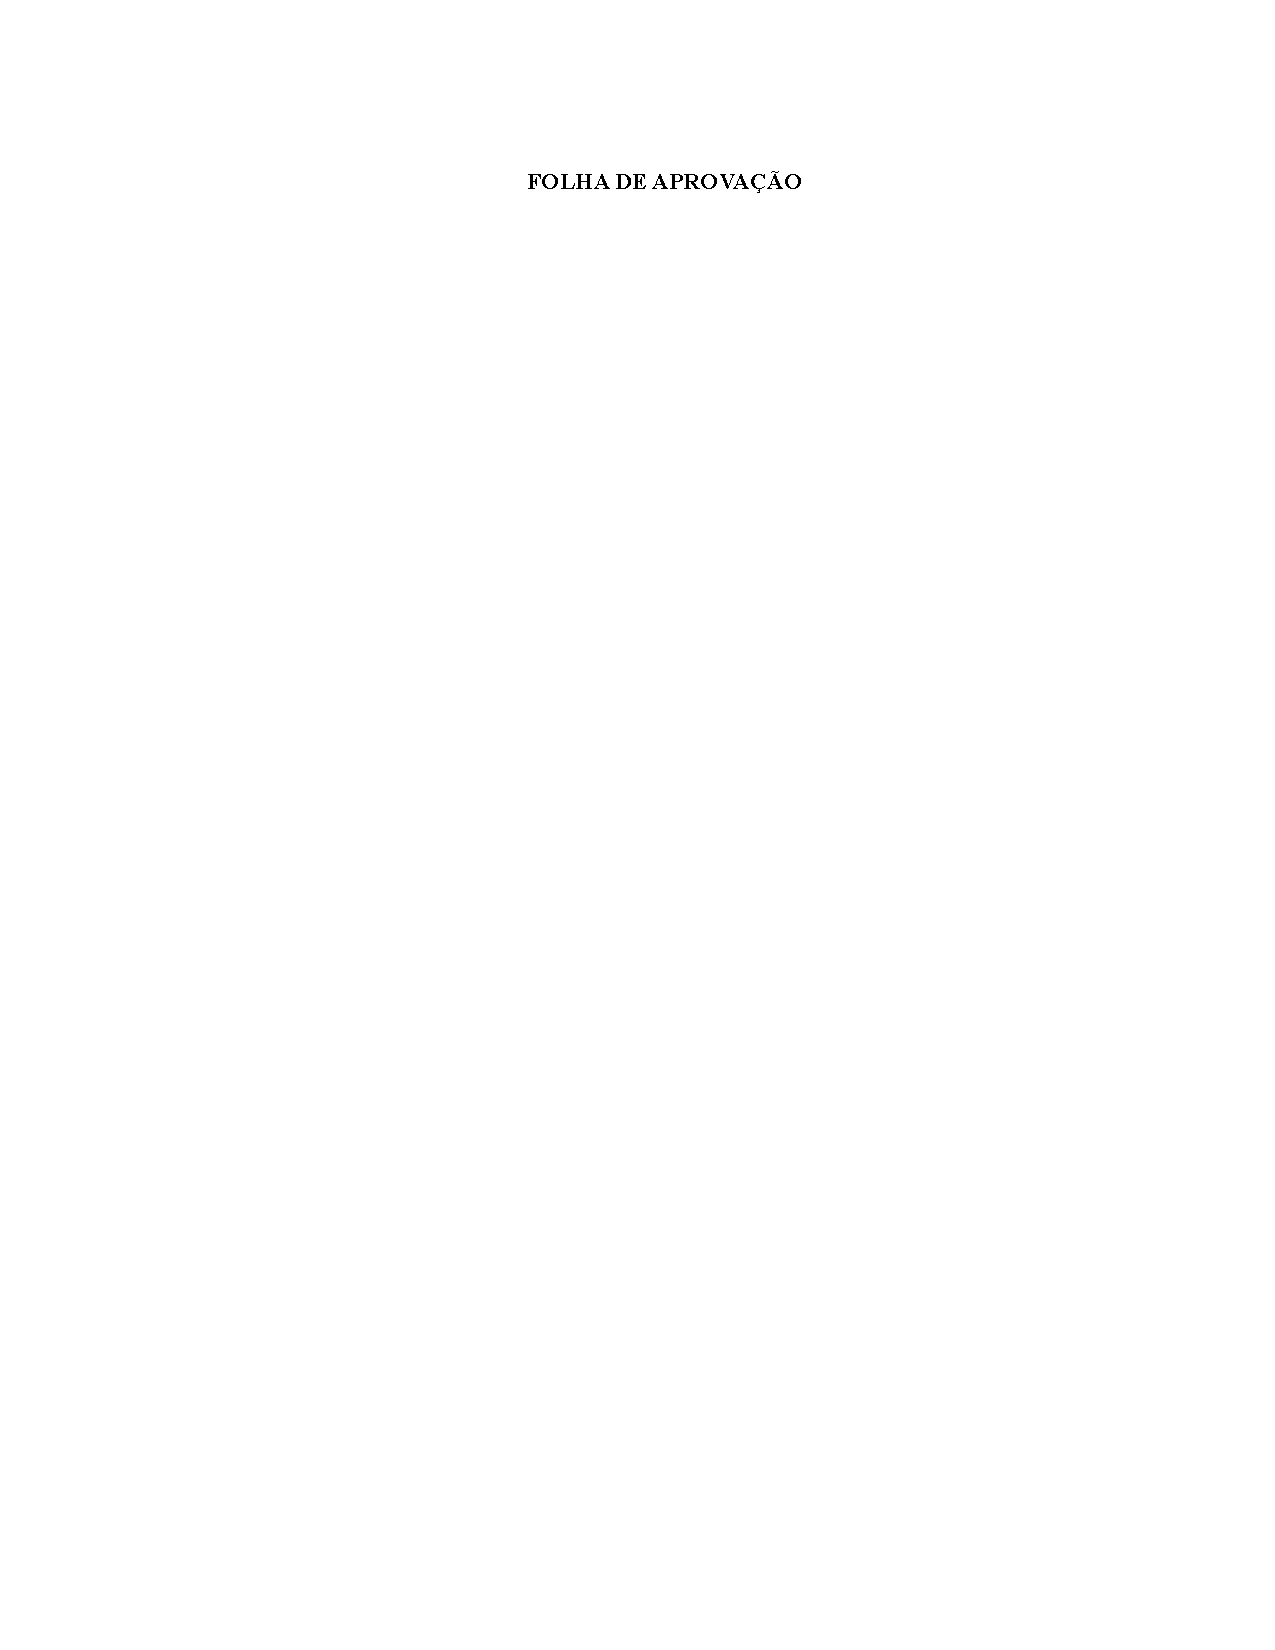
\includepdf[scale=1.0,pages=1]{./PreTexto/folha-aprovacao.pdf} % para adicionar o pdf enviado pelo professor apenas substitua o documento folha-aprovacao.pdf dentro da pasta PreTexto

%% Dedicatória
% %%%% DEDICATÓRIA
%%
%% Texto em que o autor presta homenagem ou dedica seu trabalho.

\begin{dedicatoria}%% Ambiente dedicatoria
Dedico este trabalho a minha família e aos meus amigos, pelos momentos de ausência.
\end{dedicatoria}
%% Comente para remover este item

%% Agradecimentos
% %%%% AGRADECIMENTOS
%%
%% Texto em que o autor faz agradecimentos dirigidos àqueles que contribuíram de maneira relevante à elaboração do trabalho.

\begin{agradecimentos}%% Ambiente agradecimentos

Certamente estes parágrafos não irão atender a todas as pessoas que fizeram parte dessa importante fase de minha vida. Portanto, desde já peço desculpas àquelas que não estão presentes entre essas palavras, mas elas podem estar certas que fazem parte do meu pensamento e de minha gratidão. 

Agradeço ao(a) meu(minha) orientador(a) Prof.(a) Dr.(a) Nome Completo, pela sabedoria com que me guiou nesta trajetória.

Aos meus colegas de sala.

A Secretaria do Curso, pela cooperação.

Gostaria de deixar registrado também, o meu reconhecimento à minha família, pois acredito que sem o apoio deles seria muito difícil vencer esse desafio. 

Enfim, a todos os que por algum motivo contribuíram para a realização desta pesquisa.


Espaço destinado aos agradecimentos (elemento opcional). Folha que contém manifestação de reconhecimento a pessoas e/ou instituições que realmente contribuíram com o(a) autor(a), devendo ser expressos de maneira simples.

Não devem ser incluídas informações que nominem empresas ou instituições não nominadas no trabalho.

Se o aluno recebeu bolsa de fomento à pesquisa, informar o nome completo da agência de fomento. Ex: Capes, CNPq, Fundação Araucária, UTFPR, etc. Incluir o número do projeto após a agência de fomento. Este item deve ser o último.

Atenção: não utilizar este exemplo na versão final. Use a sua criatividade!

\end{agradecimentos}
%% Comente para remover este item

%% Epígrafe
% %%%% EPÍGRAFE
%%
%% Texto em que o autor apresenta uma citação, seguida de indicação de autoria, relacionada com a matéria tratada no corpo do
%% trabalho.

\begin{epigrafe}%% Ambiente epigrafe

    EPÍGRAFE

\end{epigrafe}
%% Comente para remover este item

%% Resumo
%%%% RESUMO
%%
%% Apresentação concisa dos pontos relevantes de um texto, fornecendo uma visão rápida e clara do conteúdo e das conclusões do
%% trabalho.


\begin{resumoutfpr}%% Ambiente resumoutfpr
  Esta monografia explora a viabilidade e desenvolvimento do protótipo de um multimedidor de baixo custo. Nos laboratórios da Universidade Tecnológica Federal do Paraná, são realizados testes com a finalidade de aprendizado dos alunos do curso de Engenharia Elétrica e demais. Para tanto, são necessários equipamentos de metrologia, além dos circuitos a serem analizados. Para tanto, propõe-se um multimedidor osciloscópio com comunicação \textit{WiFi} para fazer medidas dos vários experimentos promovidos nos laboratórios. Visando ser o mais simples e didático possível, a integração da interface homem-máquina se dá pela tela de um \textit{smartphone} conectado ao dispositivo, tornando assim possível a visualização de ondas, além das medidas relevantes aos projetos. Este protótipo, composto por \textit{Hardware}, \textit{Software} e \textit{Firmware} é desenvolvido em sua totalidade utilizando-se plataformas \textit{Open-Source} disponibilizadas e também tem todos os seus materiais discretizados, visando-se a maior replicabilidade possível. ****testes e conclusão****
\end{resumoutfpr}
%% Comente para remover este item

%% Abstract
%%%% ABSTRACT
%%
%% Versão do resumo para idioma de divulgação internacional.

\begin{abstractutfpr}%% Ambiente abstractutfpr
This undergraduate thesis explores the feasibility and development of a low-cost multimeter prototype. In the laboratories of the Federal Technological University of Paraná, tests are conducted with the aim of providing practical learning to students in the Electrical Engineering program and related fields. For the execution of these experiments, the use of metrology equipment is essential, along with the circuits that will be analyzed.
In this context, the development of an oscilloscope multimeter with communication via WiFi is proposed, capable of performing measurements in various experiments conducted in the laboratories. The project was designed to be simple and educational, allowing the integration of the human-machine interface through the screen of a smartphone or computer connected to the device, thus enabling the visualization of waveforms and the acquisition of measurements relevant to the projects.
The prototype consists of hardware, software, and firmware, developed entirely using open source platforms. Furthermore, all its components have been thoroughly discretized, aiming to maximize the replicability of the project.
It was possible to validate the prototype regarding its current and voltage scales as proposed, with results shown on browser, being possible to measure them simultaniously with very close results to conventional equipment.
The concept of modularity was also explored in the system's structure, aiming to reduce the complexity, facilitate assembly and maintenance of the equipment, but it was not implemented. That being said, future development is necessary to make it possible to measure more than a single phase utilizing replicas of the device.
\end{abstractutfpr}%% Comente para remover este item

%% Lista de algoritmos
%\incluirlistadealgoritmos%% Comente para remover este item

%% Lista de ilustrações
\incluirlistadeilustracoes%% Comente para remover este item

%% Lista de Fotografias
% \incluirlistadefotografias %% Comente para remover este item

%% Lista de Gráficos
% \incluirlistadegraficos %% Comente para remover este item

%% Lista de tabelas
\incluirlistadetabelas%% Comente para remover este item

%% Lista de quadros
% \incluirlistadequadros

%% Listagem de códigos fonte
% \incluirlistadecodigosfonte

%% Lista de abreviaturas, siglas e acrônimos
\incluirlistadeacronimos{glossaries}%% Opções: "glossaries" (pacote) ou "file" (arquivo) ou "none" (desabilita)

%% Lista de símbolos
\incluirlistadesimbolos{nomencl}%% Opções: "nomencl" (pacote) ou "file" (arquivo) ou "none" (desabilita)

%% Sumário
\incluirsumario%% Comente para remover este item

%% Formatação de páginas de elementos textuais
\textual%% Não comente esta linha

%% Parte
% \part{Introdução}%% Comente para remover este item

%% Capítulo introdução - obrigatório
%%%% CAPÍTULO 1 - INTRODUÇÃO
%%
%% Deve apresentar uma visão global da pesquisa, incluindo: breve histórico, importância e justificativa da escolha do tema,
%% delimitações do assunto, formulação de hipóteses e objetivos da pesquisa e estrutura do trabalho.

%% Título e rótulo de capítulo (rótulos não devem conter caracteres especiais, acentuados ou cedilha)
\chapter{Introdução}\label{cap:introducao}

Um texto curto apresentando o capítulo.

\caixa{Atenção}{Para utilizar esse template é obrigatória a leitura do conteúdo do arquivo \texttt{readme.md}, que está neste projeto!}

\section{Considerações iniciais}\label{sec:consideracoesIniciais}

As considerações iniciais compõem um texto curto e geral apresentando uma visão geral e sucinta do assunto principal relacionado ao trabalho e a inserção do objeto de pesquisa nesse assunto \cite{Moore:2000:CMC:333067.333074}.

Em relação ao assunto, o apresentado nesta seção pode estar relacionado a trabalhos de outros autores ou ao assunto que fornece a fundamentação (motivação) para o trabalho a ser desenvolvido. Se o assunto está relacionado a trabalhos de outros autores, a contribuição do trabalho é definida em relação ao que já foi pesquisado nesse assunto. Se o assunto será utilizado para embasamento do que será proposto, explicitar como o trabalho se insere nesse assunto. A contribuição pode, ainda, estar relacionada a uma necessidade de mercado ou a uma oportunidade decorrente de algum problema real para o qual se pretender propor uma solução. Nesse caso, o assunto fornece um contexto teórico de suporte para o problema e/ou a solução.

O importante nesta seção é deixar claro do que se trata o trabalho (assunto ou tema), identificar o objeto de pesquisa, como será encaminhada a solução (procedimento metodológico, tecnologias, ferramentas utilizadas) e o que se pretende ao final do trabalho, sem explicitar a solução e os resultados.

\caixa{Atenção}{As seções a seguir são sugestões, converse com o seu orientador para ver quais seções devem ter em seu trabalho!}

\section{Objetivos}\label{sec:objetivos}

Um texto curto\footnote{Teste de nota de rodapé 1.} apresentando a seção.

\subsection{Objetivo geral}\label{subsec:objetivoGeral}

O objetivo geral se refere ao resultado do trabalho realizado, enfatizando o que esse trabalho deixa para a comunidade acadêmica, para a sociedade e/ou para o ambiente profissional. Deve ser apresentado de forma a abranger o resultado principal do teste.

O objetivo geral e os específicos devem iniciar com verbo. Sugere-se que o objetivo geral contenha no máximo 3 (três) linhas, conforme exemplo abaixo:

Desenvolver um protótipo de um sistema de software para determinar a capacidade produtiva de pequenas empresas com base em estudos de cronoanálise industrial para pequenas empresas com produção em série.

\subsection{Objetivos específicos (opcional)}\label{subsec:objetivosEspecificos}

Os objetivos específicos são opcionais, ou seja, somente devem ser apresentados se caracterizarem resultados parciais gerados a partir do objetivo geral, os quais sejam considerados úteis para a comunidade acadêmica, para a sociedade ou para o ambiente profissional. Uma observação importante é que os resultados sejam passíveis de comprovação, ou seja, se o objetivo for: “Oferecer agilidade e confiabilidade aos processos gerenciais da empresa”, significa que o trabalho deverá realizar testes com relação a esses atributos, cujos resultados deverão ser apresentados nas discussões do trabalho.

Destaca-se que os objetivos específicos não incluem as etapas do processo de desenvolvimento de software (realizar a modelagem, a análise, o projeto...) ou outras atividades necessárias para alcançar o objetivo geral, como, estudar as tecnologias necessárias para modelagem e implementação do sistema. Dentre as exceções estão a realização de estudos, procedimentos, métodos e técnicas considerados inéditos e de relevância para outros trabalhos a serem realizados na mesma área. Contudo, o resultado deste estudo deve ser documentado de forma que seja conhecimento disponibilizado para quem lê o trabalho.

\section{Justificativa}\label{sec:justificativa}

Justificar o objeto de pesquisa (o que será feito) e a forma de resolução do problema (como fazer). A forma de resolução pode estar centrada no método, nas tecnologias, no uso de conceitos (fundamentação teórica).

A Justificativa explicita porque desenvolver o referido trabalho, como o mesmo se insere no contexto de pesquisa, de produção científica. Pode incluir o porquê utilizar as tecnologias e ferramentas indicadas, a contribuição em termos de inovação ou mesmo de aprendizado.

O trabalho não precisa ser justificado em decorrência de ser inovador ou por ter gerado uma significativa contribuição ao conhecimento na área em que o mesmo se insere. Pode referir-se simplesmente à aplicabilidade de conhecimentos adquiridos durante o curso. Sendo assim, a justificativa não deve ser elaborada considerando um mercado a ser atingido e sim com relação ao uso de tecnologias aprendidas e/ou estudadas, o conhecimento e aprendizado do aluno e a aplicabilidade do trabalho desenvolvido.

\section{Estrutura do trabalho}\label{sec:estruturaTrabalho}

A estrutura do trabalho contém uma relação dos capítulos e uma descrição sucinta do que cada um deles contém. Esta seção fornece uma visão geral do trabalho no sentido da sua estrutura em capítulos\footnote{Teste de nota de rodapé 2.}.

\caixa{Atenção}{O OverLeaf está demorando muito para compilar o modelo com o Capítulo de Exemplos, que explica como usar o LaTeX. Assim, esse capítulo foi removido (está comentado para não compilar), mas há um arquivo chamado \texttt{exemploPDF.pdf}, na raiz do projeto, que contém esse capítulo de exemplos!}
%% Comente para remover este item

%% Andrey - Referências bibliográficas ou Estado da arte
\chapter{Revisão Bibliográfica e Estado da Arte}
\label{cap:refbib}

Neste trabalho, o objetivo foi desenvolver um multímetro capaz de medir tensão e corrente simultaneamente e enviar os dados para um smartphone por meio de uma conexão wifi. Considerando essa proposta, foram analisadas duas opções para servir como base: um multimedidor e um multímetro.

O multimedidor é um dispositivo geralmente trifásico, que permite a medição simultânea de tensão e corrente, exibindo as formas de onda em um display. Possui três ou mais canais simultâneos. No entanto, apresenta a limitação de possuir apenas um referencial de medição, com resolução na ordem de 1V nos modelos mais baratos e 0,1V nos modelos mais caros, repetindo-se esses valores para a resolução da corrente \cite{fluke434}.

Por outro lado, o multímetro é um dispositivo monofásico que permite a medição de apenas um canal por vez, como tensão, corrente, resistência, capacitância, entre outros. Ele não exibe as curvas na tela, fornecendo apenas os valores. A resolução varia, sendo que nos modelos mais simples pode chegar a 0,1 mV, enquanto a resolução da corrente é da ordem de 1uA \cite{et1100}.

Considerando que o dispositivo deve ser utilizado como uma ferramenta didática em sala de aula, é essencial que a resolução seja adequada para o bom aproveitamento das disciplinas. Além disso, a apresentação das formas de onda também é relevante. Assim, optou-se por uma abordagem que combina características de ambos os dispositivos, utilizando os diagramas de blocos para identificar as funcionalidades e suas relações com o dispositivo a ser produzido.

Para o multimedidor, foi utilizado o diagrama de blocos do \textit{oZm3} (\autoref{fig:ozm3flowchart}), um produto \textit{open source} (projeto aberto) já introduzido no mercado, sendo uma versão trifásica de outro, também \textit{open source} chamado \textit{(openZmeter)}. Ambos possuem interface de apresentação dos dados via uma página do navegador de um celular ou computador.

\begin{figure}[h]
    \caption{Diagrama de blocos do multimedidor trifásico oZm3}
    \label{fig:ozm3flowchart}
    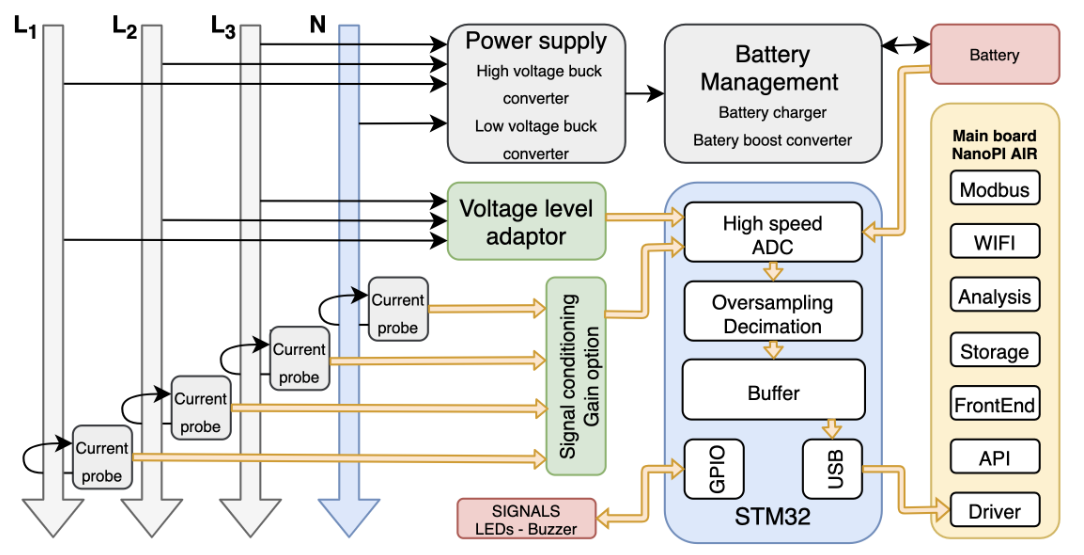
\includegraphics[width=0.8\textwidth]{figuras/openzmeter-diagrama.png}
    \fonte{\cite{3ph-ozm}}
\end{figure}

Para o multímetro, foi utilizado um diagrama de blocos (\autoref{fig:multimeterflowchart}) disponível no site da (CITAÇÃO) \textit{Texas Instruments}, que explica o funcionamento de um produto completo.

\begin{figure}[h]%% Ambiente figure
    %\captionsetup{width=0.55\textwidth}%% Largura da legenda
    \caption{Exemplo de um Diagrama de Blocos de um Multímetro de Bancada}%% Legenda
    \label{fig:multimeterflowchart}%% Rótulo
    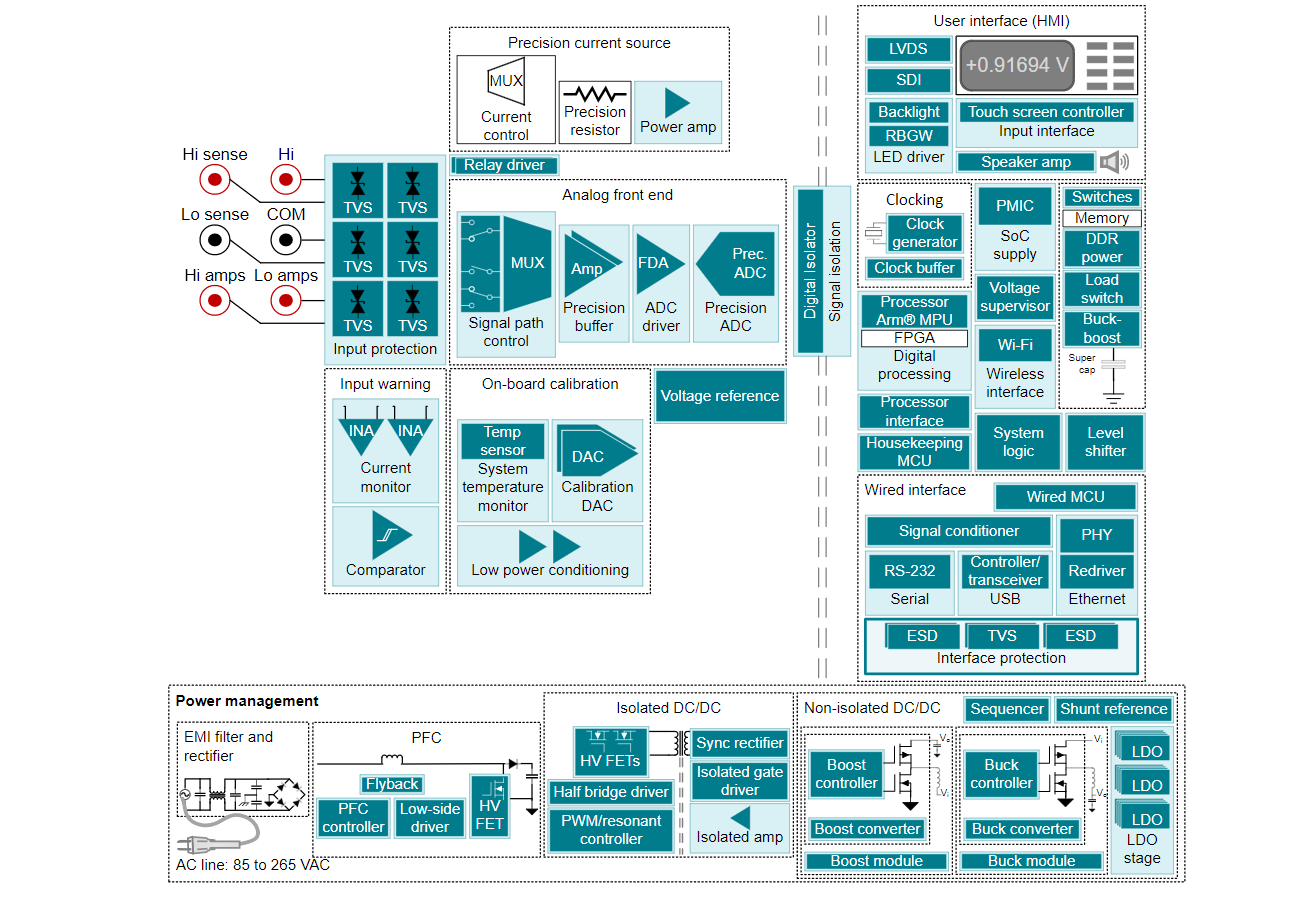
\includegraphics[width=1\textwidth]{flowchart}%% Dimensões e localização
    \fonte{Texas Instruments}%% Fonte
\end{figure}

Sobre o estado da arte, existem diversos dispositivos que atendem a necessidades diferentes, como por exemplo, segurança (CAT rating), resolução, precisão ou até mesmo confiabilidade de leitura em condições de temperaturas elevadas, entre vários outros. Adicionalmente, existem também inúmeros fornecedores, tanto regionais, nacionais como internacionais, salientando a diversidade de produtos.

Dispositivos como o Fluke 28-II EX possuem boa métrica de confiabilidade e também são portáteis, além de fazerem medidas em \textit{True-RMS} (True Root Mean Square). Este dispositivo é muito benquisto, tendo boas avaliações no mundo inteiro.

\begin{figure}[htb]%% Ambiente figure
    %\captionsetup{width=0.55\textwidth}%% Largura da legenda
    \caption{Fluke 28-II}%% Legenda
    \label{fig:Fluke28-II}%% Rótulo
    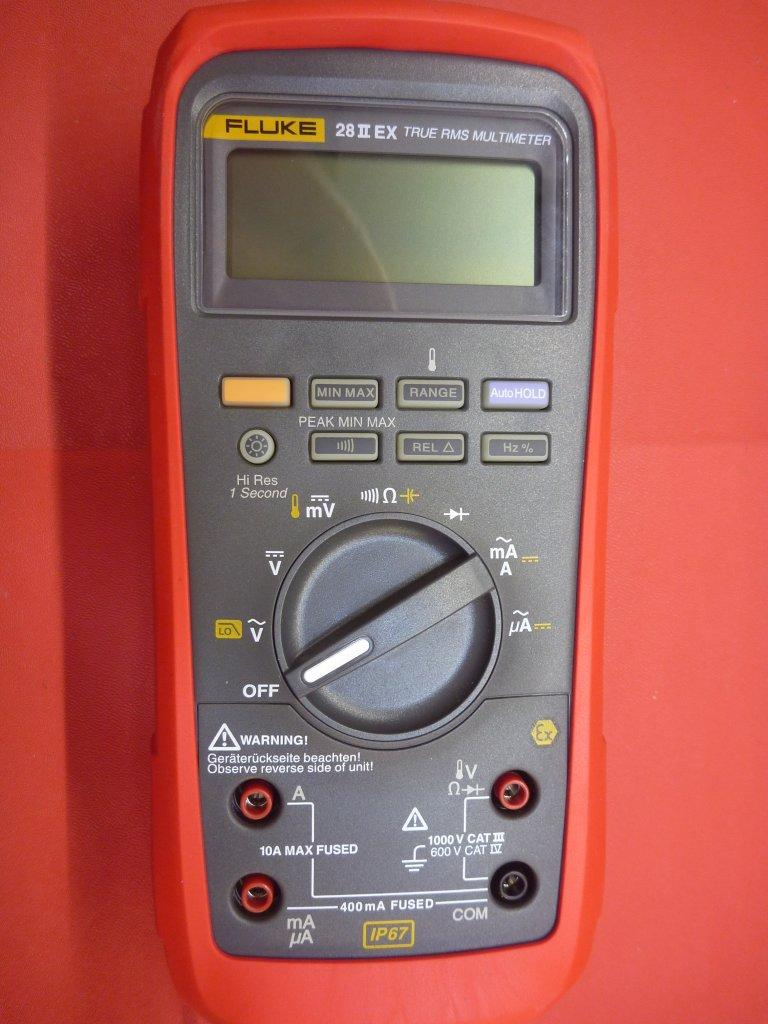
\includegraphics[scale=0.4]{Fluke28-II}%% Dimensões e localização
    \fonte{fluke28iixd}%% Fonte
\end{figure}

Sobre multímetros digitais, também existem aqueles que são de bancada ou \textit{benchtop}. Tais dispositivos são de uso mais específico, prezando a precisão de leitura, resolução e também contendo algumas \textit{features} a mais. Como exemplo, o DMM7510 7.5 Digit Graphical Sampling Multimeter da Tektronix é um dispositivo que porta todas as funções já explicitas e também várias outras de uso extremamente específico, como \textit{profiling} de corrente de consumo de energia em dispositivos \gls{IoT} (\textit{Internet of Things}), como mostrado na \autoref{fig:tektronixdmm}.

\begin{figure}[htb]%% Ambiente figure
    %\captionsetup{width=0.55\textwidth}%% Largura da legenda
    \caption{Gráfico de corrente de consumo de um dispositivo, feito pelo DMM7510 7.5 Digit Graphical Sampling Multimeter}%% Legenda
    \label{fig:tektronixdmm}%% Rótulo
    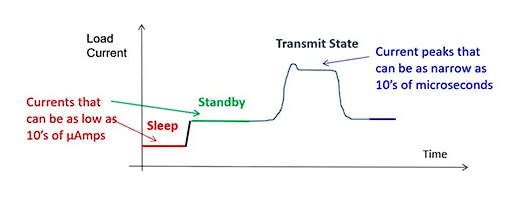
\includegraphics[scale=0.8]{tektronixdmm}%% Dimensões e localização
    \fonte{tektDMM}%% Fonte
\end{figure}

No caso de multimedidores, que são somente de uso específico industrial, alguns fornecedores e dispositivos se sobressaem, como a WEG. O MMW03, por exemplo, é um multimedidor da família MMW, fornecido pela mesma, que faz todas as medidas de grandezas elétricas no meio industrial, tem a função de parametrizá-las por meio de aplicativos \gls{IoT}, identifica sequência e falta de fases, entre outras várias funções que são benéficas para tal aplicação. 

\begin{figure}[htb]%% Ambiente figure
    %\captionsetup{width=0.55\textwidth}%% Largura da legenda
    \caption{Dispositivo MMW03}%% Legenda
    \label{fig:mmw03weg}%% Rótulo
    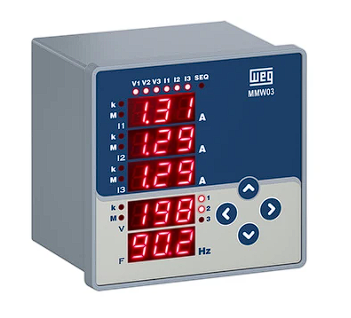
\includegraphics[scale=0.6]{mmw03weg}%% Dimensões e localização
    \fonte{WEG}%% Fonte
\end{figure}
%https://www.fluke.com/en/product/intrinsically-safe/fluke-28-ii-ex (Fluke 28-II EX)
%https://www.tek.com/en/products/keithley/digital-multimeter/dmm7510 (Benchtop DMM)
%https://www.testmart.com/webdata/mfr_pdfs/FLU/27______smeng0100.pdf (Handheld, old DMM)
%https://www.weg.net/catalog/weg/BR/pt/Automa%C3%A7%C3%A3o-e-Controle-Industrial/Controls/Prote%C3%A7%C3%A3o-de-Circuitos-El%C3%A9tricos/Multimedidores-e-Medidores-Inteligentes/Multimedidor-de-Grandezas-El%C3%A9tricas-MMW03/MULTIMEDIDOR-MMW03/p/14386964 (Multimedidor)

%% Capítulo
%%%% CAPÍTULO 2 - REVISÃO DA LITERATURA (OU REVISÃO BIBLIOGRÁFICA, ESTADO DA ARTE, ESTADO DO CONHECIMENTO)
%%
%% O autor deve registrar seu conhecimento sobre a literatura básica do assunto, discutindo e comentando a informação já publicada.
%% A revisão deve ser apresentada, preferencialmente, em ordem cronológica e por blocos de assunto, procurando mostrar a evolução do tema.
%% Título e rótulo de capítulo (rótulos não devem conter caracteres especiais, acentuados ou cedilha)
\chapter{Referencial Teórico}\label{cap:referencialTeorico}

Este capítulo será dedicado a explicar como funcionam as várias partes envolvidas na construção e funcionamento de um multímetro digital e/ou multimedidor.

Neste trabalho, o objetivo é desenvolver um multímetro capaz de medir tensão e corrente simultaneamente e enviar os dados para um \textit{smartphone} por meio de conexão sem fio. Considerando essa proposta, foram analisadas três opções para servir como base: um multimedidor, um multímetro e um osciloscópio.

O multimedidor é um dispositivo geralmente trifásico, que permite a medição simultânea de tensão e corrente, exibindo as formas de onda em um display. Possui três ou mais canais simultâneos. No entanto, apresenta a limitação de possuir apenas um referencial de medição e resolução na ordem de 1 V nos modelos mais baratos e 0,1 V nos modelos mais caros. A mesma limitação (e valores) acontece para a resolução da corrente \cite{fluke434}.

Por outro lado, o multímetro é um dispositivo monofásico que permite a medição de apenas um canal por vez, como tensão, corrente, resistência, capacitância, entre outros. Este não exibe as curvas na tela, fornecendo apenas valores. A resolução varia, sendo que nos modelos mais simples pode chegar a 0,1 mV, enquanto a resolução da corrente é da ordem de 1µA \cite{et1100}.

O osciloscópio, por sua vez, é uma ferramenta amplamente utilizada para a visualização gráfica de sinais elétricos, oferecendo uma leitura detalhada das variações de tensão ao longo do tempo. Com ele, é possível medir sinais com alta precisão e analisar eventos rápidos que não seriam capturados por multímetros convencionais. Equipado com múltiplos canais, o osciloscópio permite a comparação simultânea de diferentes sinais. Sua resolução de tela varia dependendo do modelo, indo de 800x600 até 1920x1080 pixels, o que proporciona uma visualização clara de formas de onda complexas. Além disso, os sistemas de disparo \textit{(triggering)} garantem a captura e estabilização de sinais repetitivos, essenciais para análises em tempo real \cite{keysight-oscilloscope-guide}.

Considerando que o dispositivo deve ser utilizado como uma ferramenta didática em sala de aula, é essencial que a resolução seja adequada para o bom aproveitamento das disciplinas. Além disso, a apresentação das formas de onda também é relevante. Assim, optou-se por uma abordagem que combina características dos dispositivos.

Para o multimedidor, foi utilizado o diagrama de blocos do \textit{oZm3} (\autoref{fig:ozm3flowchart}), um produto \textit{open source} (projeto aberto) já introduzido no mercado, sendo uma versão trifásica de outro, também \textit{open source} chamado \textit{(openZmeter)}. Ambos possuem interface de apresentação dos dados via uma página do navegador de um celular ou computador.

\begin{figure}[htb!]
    \caption{Diagrama de blocos do multimedidor trifásico oZm3}
    \label{fig:ozm3flowchart}
    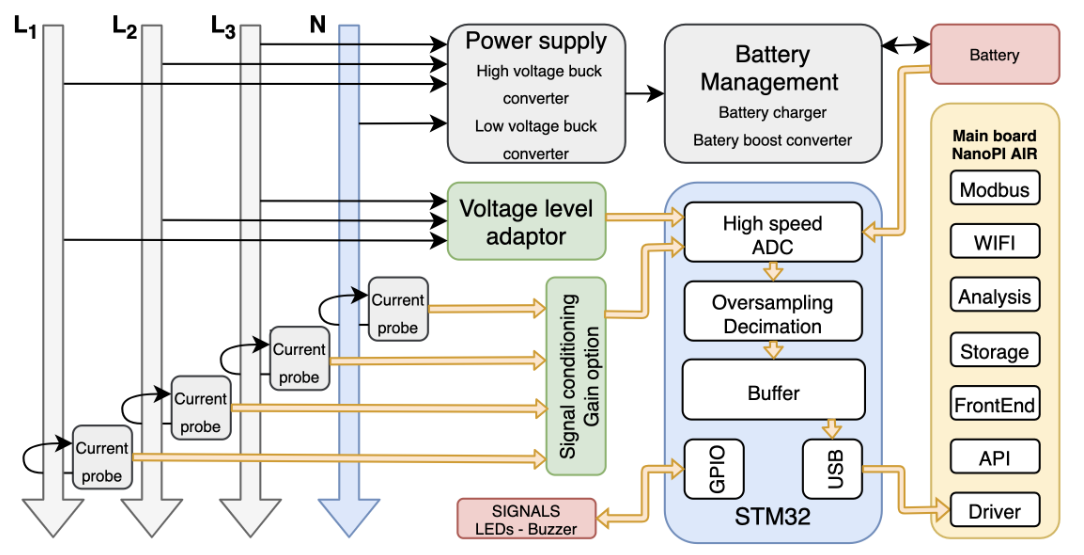
\includegraphics[width=0.8\textwidth]{figuras/openzmeter-diagrama.png}
    \fonte{\cite{3ph-ozm}}
\end{figure}

Para o multímetro, foi utilizado um diagrama de blocos (\autoref{fig:multimeterflowchart}) disponível no site da \textit{Texas Instruments}, que explica o funcionamento de um produto completo.

\begin{figure}[htb!]%% Ambiente figure
    %\captionsetup{width=0.55\textwidth}%% Largura da legenda
    \caption{Exemplo de um Diagrama de Blocos de um Multímetro de Bancada}%% Legenda
    \label{fig:multimeterflowchart}%% Rótulo
    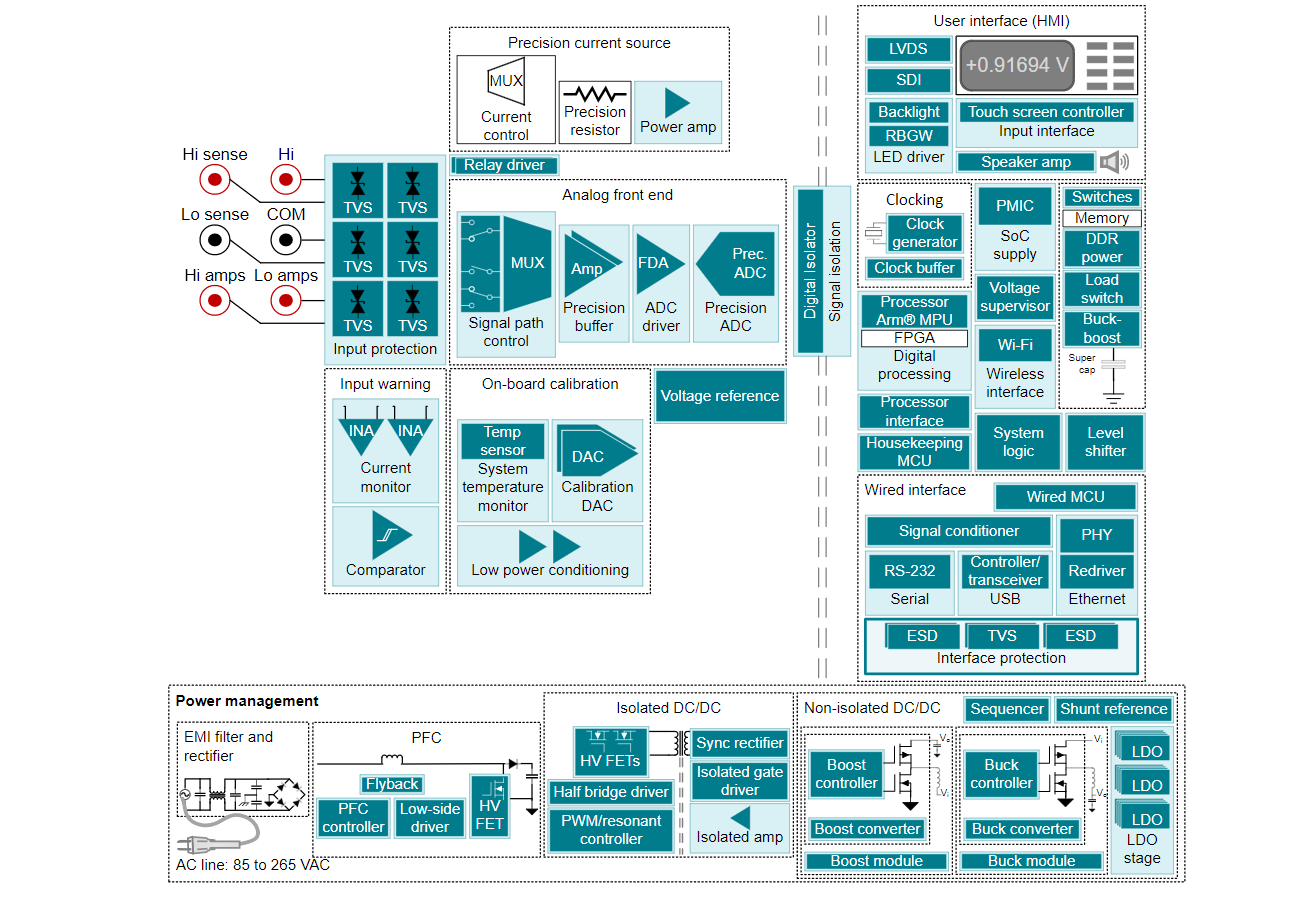
\includegraphics[width=1\textwidth]{flowchart}%% Dimensões e localização
    \fonte{\cite{DMMTI}}%% Fonte
\end{figure}

Sobre o padrão comercial, existem diversos dispositivos que atendem a necessidades diferentes, como por exemplo, segurança (CAT rating), resolução, precisão ou até mesmo confiabilidade de leitura em condições de temperaturas elevadas, entre vários outros. Adicionalmente, existem também inúmeros fornecedores, tanto regionais, nacionais como internacionais, salientando a diversidade de produtos.

Dispositivos como o representado na \autoref{fig:Fluke28-II} possuem boa métrica de confiabilidade e também são portáteis, além de provirem medidas em \textit{True-RMS} (\textit{True Root Mean Square}). Este dispositivo é muito benquisto, tendo boas avaliações no mundo inteiro.

\begin{figure}[htb!]%% Ambiente figure
    %\captionsetup{width=0.55\textwidth}%% Largura da legenda
    \caption{Fluke 28-II}%% Legenda
    \label{fig:Fluke28-II}%% Rótulo
    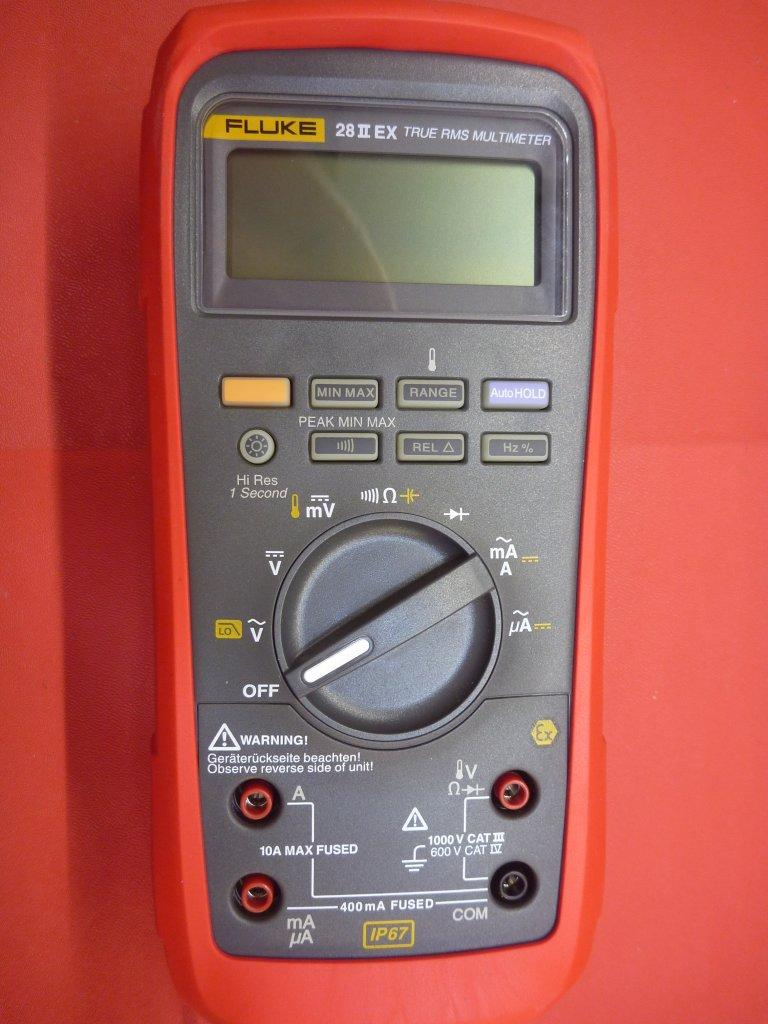
\includegraphics[scale=0.4]{Fluke28-II}%% Dimensões e localização
    \fonte{\cite{fluke28iixd}}%% Fonte
\end{figure}

Sobre multímetros digitais, também existem aqueles que são de bancada ou \textit{benchtop}. Tais dispositivos são de uso mais específico, prezando a precisão de leitura, resolução e também contendo algumas \textit{features} a mais. Como exemplo, o DMM7510 7.5 \textit{Digit Graphical Sampling Multimeter} da Tektronix é um dispositivo que porta todas as funções já explicitas e também várias outras de uso extremamente específico, como \textit{profiling} de corrente de consumo de energia em dispositivos \gls{IoT} (\textit{Internet of Things}), como mostrado na \autoref{fig:tektronixdmm}.

\begin{figure}[htb!]%% Ambiente figure
    %\captionsetup{width=0.55\textwidth}%% Largura da legenda
    \caption{Gráfico de corrente de consumo de um dispositivo, feito pelo DMM7510 7.5 Digit Graphical Sampling Multimeter}%% Legenda
    \label{fig:tektronixdmm}%% Rótulo
    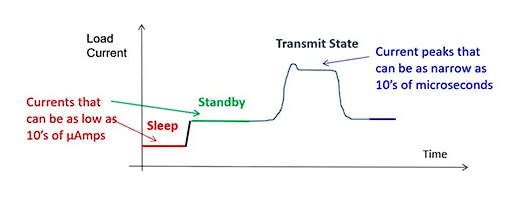
\includegraphics[scale=0.8]{tektronixdmm}%% Dimensões e localização
    \fonte{tektDMM}%% Fonte
\end{figure}

No caso de multimedidores, que são somente de uso específico industrial, alguns fornecedores e dispositivos se sobressaem, como a WEG. O dispositivo da \autoref{fig:mmw03weg} é um multimedidor da família MMW, fornecido pela mesma. O multimedidor é capaz de coletar todas as medidas de grandezas elétricas no meio industrial, tem a função de parametrizá-las por meio de aplicativos \gls{IoT}, identifica sequência e falta de fases, entre outras várias funções que são benéficas para tal aplicação.

\begin{figure}[htb!]%% Ambiente figure
    %\captionsetup{width=0.55\textwidth}%% Largura da legenda
    \caption{Dispositivo MMW03}%% Legenda
    \label{fig:mmw03weg}%% Rótulo
    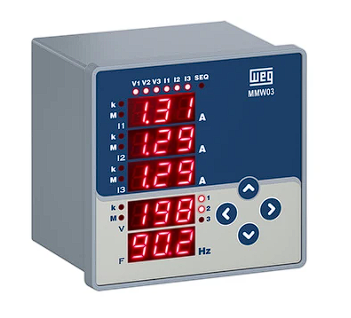
\includegraphics[scale=0.6]{mmw03weg}%% Dimensões e localização
    \fonte{WEG}%% Fonte
\end{figure}

%Input Protection > Pathing > Aquisição de Sinal > ADC > Referência de Tensão > Input Warning > MCU > Interfaceamento > Power Supply > Calibração

% RAFAEL --------------------------------------------------------------------------------------------------------
%Input Protection
\section{Proteção de Entrada}\label{sec:InputProtection}

Proteção de entrada é um assunto extremamente abrangente quando se trata de circuitos eletrônicos. Dependendo da função que este tenha que exercer, existem infinitas topologias que podem ser consideradas. Algumas exigências, porém, são comuns, como a necessidade de um circuito de proteção contra descargas eletrostáticas, ou \gls{ESD} (\textit{Electrostatic Discharge}). Tais descargas podem entregar picos de tensão extremamente altos, chegando até 30 kV, o que é extremamente danoso a qualquer circuito que use semicondutores. Pulsos de pico tão alto quanto 2500 V (Volts) já são o suficiente para danificar a maioria dos circuitos eletrônicos. Notoriamente, seres humanos são capazes de entregar descargas de até 20 kV por consequência da capacitância inata à sua fisiologia \cite{ONsemicondTVS2}.

\subsection{ESD}\label{subsec:electrostaticDischarge}
Esse tipo de proteção é necessária para circuitos que fazem interface com o meio físico e normalmente é exercida por um circuito básico de componentes \gls{TVS} (\textit{Transient Voltage Suppressor}). Os dispositivos semicondutores mais simples (e também regularmente) utilizados para exercer esta função são diodos Zener \cite{IPblog}.

Ao serem submetidos a uma tensão maior que à especificada como limite de operação do circuito a ser protegido, diodos Zener apresentam uma resistência baixa, fechando a passagem de corrente entre o circuito e o \textit{ground} do equipamento. Este circuito pode apresentar uma configuração unidirecional ou bidirecional, dependendo da necessidade do circuito a ser protegido \cite{TIESD}.

As figuras \ref{fig:tvsUnidirecional} e \ref{fig:tvsBidirecional} demonstram a utilização básica de tal circuito e o conceito por trás da tensão de ruptura de tal semicondutor.

\begin{figure}[htb!]%% Ambiente figure
    %\captionsetup{width=0.55\textwidth}%% Largura da legenda
    \caption{Exemplo de uso TVS Unidirecional}%% Legenda
    \label{fig:tvsUnidirecional}%% Rótulo
    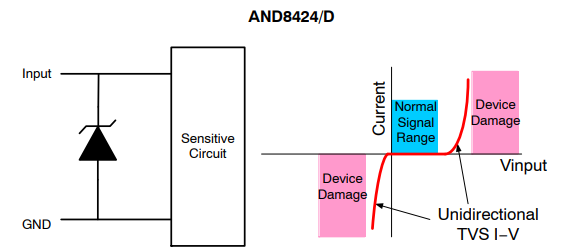
\includegraphics[scale=0.8]{tvs-unidirectional}%% Dimensões e localização
    \fonte{\cite{ONsemicondTVS}}%% Fonte
\end{figure}

\begin{figure}[htb!]%% Ambiente figure
    %\captionsetup{width=0.55\textwidth}%% Largura da legenda
    \caption{Exemplo de uso TVS Bidirecional}%% Legenda
    \label{fig:tvsBidirecional}%% Rótulo
    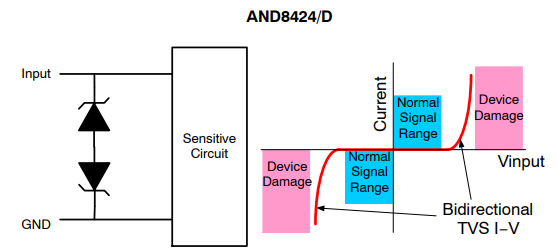
\includegraphics[scale=0.8]{tvs-bidirectional}%% Dimensões e localização
    \fonte{\cite{ONsemicondTVS}}%% Fonte
\end{figure}

\subsection{Proteção Específica para Equipamentos de Medição de Sinais Elétricos}\label{subsec:especProtec}

Primeiramente, se faz necessário explicar sobre a classificação de proteção em relação a equipamentos elétricos. A classificação mais robustamente utilizada é a CAT, que funciona conforme a \autoref{fig:CATrating}. Os numerais indicam o potencial de energia que o sistema pode entregar caso ocorra um curto-circuito ou um transiente de tensão, \textit{i.e.} um instrumento CAT III tem que estar protegido contra transientes muito maiores que um dispositivo CAT II.

Dispositivos CAT IV devem estar protegidos a nível de distribuição de energia, pois estes serão utilizados em conexão entrada de energia de uma facilidade. Dispositivos CAT III devem estar protegidos a nível de distribuição interna (quadros de distribuição), podendo esta ser trifásica ou monofásica. Dispositivos CAT II devem estar protegidos a nível de equipamento terminal ou de uso comum, sendo estes eletrodomésticos e afins. Dispositivos CAT I devem estar protegidos a nível de circuitos eletrônicos e transformadores de baixa potência \cite{CATratingu}. %%ref: https://www.ecmweb.com/test-measurement/article/21247639/understanding-the-cat-rating-system

\begin{figure}[htb!]%% Ambiente figure
    %\captionsetup{width=0.55\textwidth}%% Largura da legenda
    \caption{Ilustração da Classificação CAT}%% Legenda
    \label{fig:CATrating}%% Rótulo
    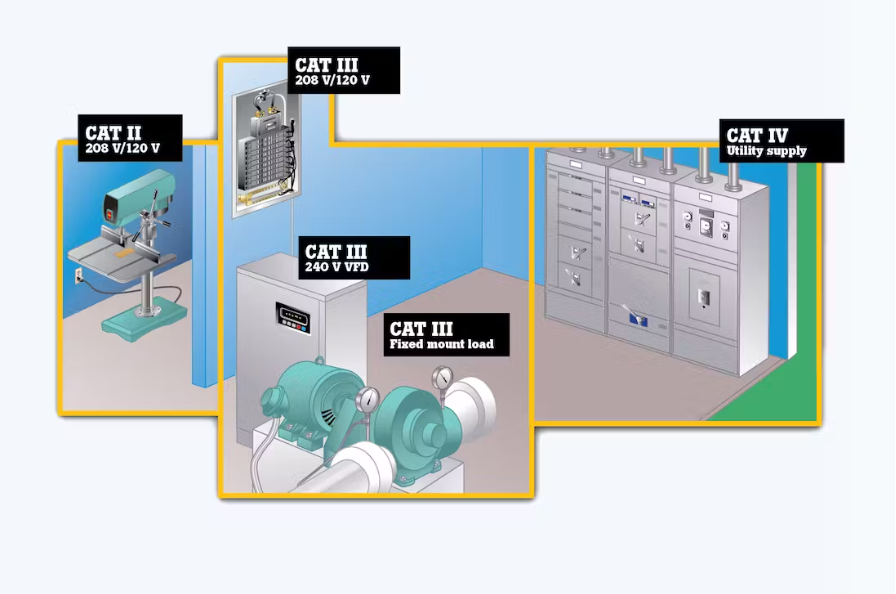
\includegraphics[scale=0.4]{CATrating}%% Dimensões e localização
    \fonte{\cite{CATratingu}}%% Fonte
\end{figure}



\subsubsection{Proteção de Entrada para Circuitos de Corrente}\label{subsec:protecaoCorrente}

O circuito de proteção para a entrada de correntes se divide em duas partes, sendo uma delas para o range de A (Amperes) e os ranges de mA e µA.

Para a entrada de Amperes, é utilizado um fusível \gls{HRC} (\textit{High Rupturing Capacity}), geralmente de 11 A e 1000 V (para se adequar à classificação CAT III, no caso do multímetro que foi estudado), para se prevenir arcos voltaicos após a queima do fusível, negando a possibilidade de uma continuação da condução de curto-circuito ou sobrecorrente. Logo após, é conectado um shunt, 0R01 $\Omega$, entre o ground e a entrada, no qual será feita a medida.

Para a entrada de mA e µA, também é utilizado um fusível \gls{HRC}, mas de 500 mA e 1000 V. Em sequência, é colocado um retificador em ponte de diodos entre o canal e o ground, para dar clamp em possíveis sobretensões (normalmente ocasionada pela utilização errônea do equipamento, colocando-se a entrada de corrente para medir tensão) até que o fusível possa atuar. Internamente, há um switch entre mA e µA \cite{fluke27manual}.

Para o switch de mA, é conectado em série um resistor shunt de 1 $\Omega$ com o shunt do range de A (0R01 $\Omega$), para ser feita a medição em uma resistência aproximada de 1 $\Omega$.

Para o switch de µA, é conectado um resistor shunt de 100 $\Omega$, no qual será feita a medição. \cite{IPblog}%%ref: https://lygte-info.dk/info/DMMDesignProtection%20UK.html

\subsubsection{Proteção de Entrada para Circuitos de Tensão}\label{subsec:protecaoTensao}

O circuito de proteção para a entrada de tensão é simples, sendo composto por um termistor \gls{PTC} (\textit{Positive Temperature Coefficient}) em série com um resistor de 10 M$\Omega$, no qual será feita a medida \cite{fluke27manual}. Esse termistor atua limitando a corrente inicial, enquanto o resistor é responsável pela medição precisa da tensão.

Para complementar essa proteção, conectado em paralelo ao resistor de 10 M$\Omega$ com o ground input, há uma série de varistores \gls{MOV} (\textit{Metal Oxide Varistor}) de rápida atuação. Esses varistores protegem contra transientes de sobretensão enquanto o termistor está esquentando e ajustando sua resistência. Embora seja possível utilizar apenas um varistor, a utilização de vários em série aumenta a distância de fuga de corrente, reduz a chance de arcos voltaicos e dissipa a energia entre os componentes, resultando em uma proteção mais eficiente \cite{flukeblog}.

Uma parte comum do design geral da \gls{PCB} (\textit{Printed Circuit Board}) são \textit{slots} de isolamento de alta tensão, que se resumem a espaços abertos entre partes da placa, que vão receber altas tensões em funcionamento indesejado, para minimizar as chances de arcos voltaicos entre partes do circuito, como destacado na \autoref{fig:exemploPCB}. %%ref: https://lygte-info.dk/info/DMMDesignProtection%20UK.html

\begin{figure}[htb!]%% Ambiente figure
    %\captionsetup{width=0.55\textwidth}%% Largura da legenda
    \caption{Fluke 28-II PCB}%% Legenda
    \label{fig:exemploPCB}%% Rótulo
    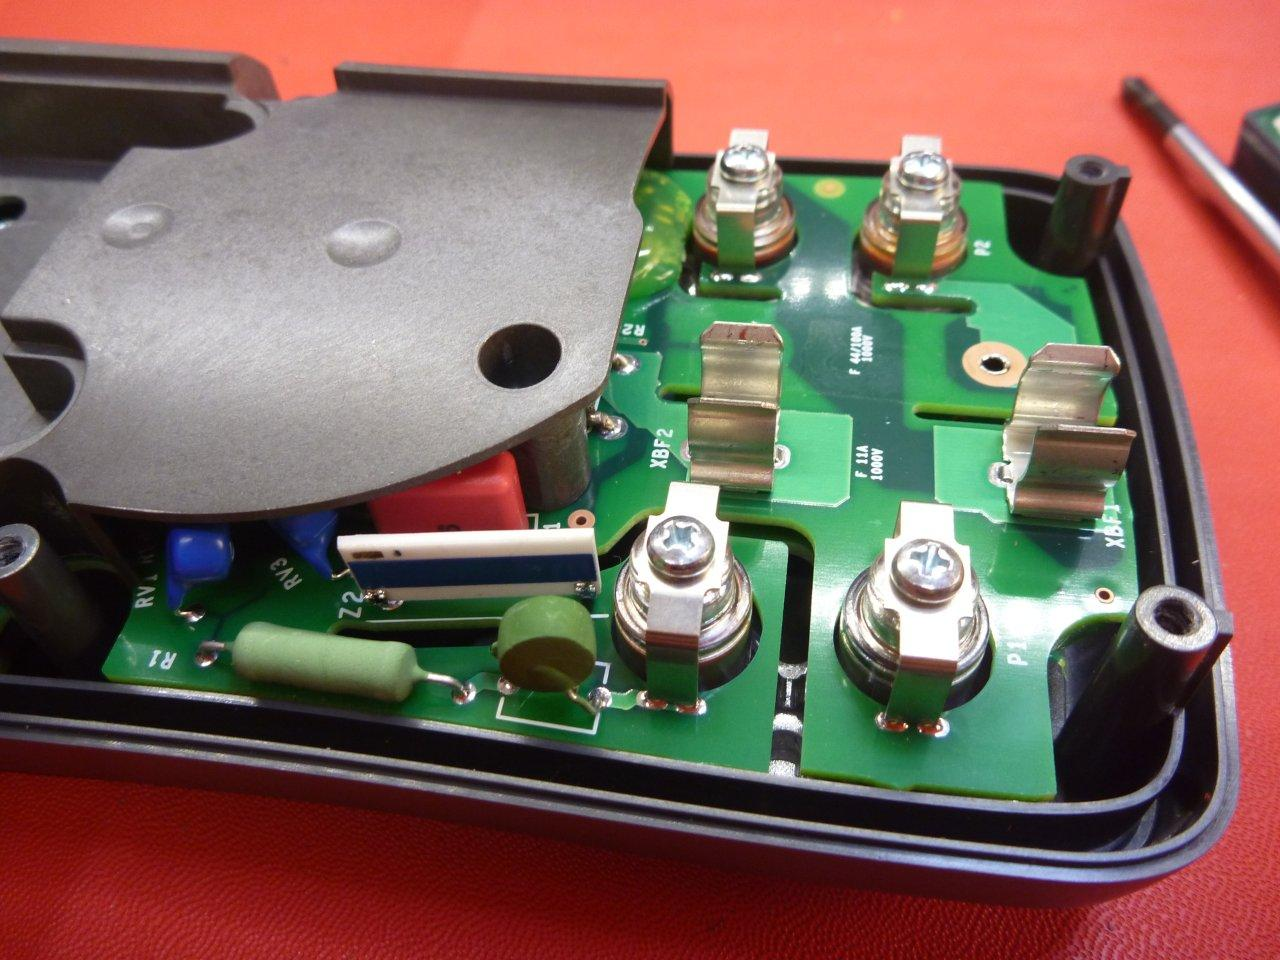
\includegraphics[scale=0.6]{divetPCB}%% Dimensões e localização
    \fonte{\cite{flukeforum}}%% Fonte
\end{figure}

%Pathing
\section{Condicionamento e Aquisição de Sinal}\label{sec:signalConditioningandPathing}

O condicionamento de sinal refere-se ao processo de ajustar e controlar o sinal de entrada que será avaliado pelo ADC (Conversor Analógico-Digital). Esse processo é essencial para garantir que o sinal fornecido ao ADC esteja dentro da faixa adequada de operação e com a qualidade necessária para uma conversão precisa. Normalmente, essa seleção de entrada é realizada por um \textit{MUX} (Multiplexador), que alterna entre diferentes sinais analógicos, ou por switches mecânicos, conforme ilustrado na \autoref{fig:Fluke28-II-switches}. Em algumas situações, pode-se empregar uma combinação desses dois métodos para otimizar a seleção e o condicionamento do sinal de acordo com as características específicas do sistema.

Além de garantir que o sinal analógico esteja dentro do intervalo correto, o condicionamento de sinal também pode envolver o uso de filtros e amplificadores para eliminar ruídos indesejados e aumentar a resolução da medição. Dessa forma, o sinal que chega ao ADC está devidamente ajustado, garantindo maior precisão e confiabilidade nos dados convertidos \cite{dmmblog}.

\begin{figure}[htb!]%% Ambiente figure
    %\captionsetup{width=0.55\textwidth}%% Largura da legenda
    \caption{Switches de um Fluke 28-II}%% Legenda
    \label{fig:Fluke28-II-switches}%% Rótulo
    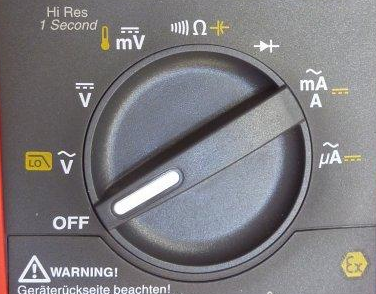
\includegraphics[scale=0.8]{Fluke28-II-switches}%% Dimensões e localização
    \fonte{\cite{flukeforum}}%% Fonte
\end{figure}

%Aquisição de Sinal
% \section{Aquisição de Sinal}\label{sec:aqSignal}

A aquisição de sinal é o processo de captura e conversão de sinais físicos em um formato adequado para análise, processamento ou armazenamento. No contexto da medição de tensão e corrente, a aquisição de sinal refere-se à captura e registro desses parâmetros elétricos em um sistema de medição, permitindo sua análise, processamento ou armazenamento em um formato adequado.

Essa pode ser realizada de diferentes maneiras, dependendo do caso. Em alguns cenários, utiliza-se sondas específicas para cada aplicação, as quais permitem capturar e registrar os parâmetros elétricos de forma precisa. Por outro lado, em certos casos, a aquisição ocorre internamente dentro do circuito do próprio medidor, proporcionando uma solução integrada e simplificada para a captura e registro dos sinais elétricos.

\subsection{Resistor Shunt}\label{subsec:resiShunt}
Neste tipo de medição, um resistor de baixo valor (< 0,1 $\Omega$) é colocado em série com o circuito no qual se deseja medir a corrente elétrica, quando esta atravessa o componente, ocorre uma queda de tensão proporcional. Essa queda de tensão pode ser então medida diretamente através de um \gls{ADC} ou amplificada e então medida para se obter os valores da corrente original \citep{curr_sens_tech}.

Para a aplicação em 3 canais independentes de corrente, torna-se necessária algum tipo de isolação. Isso pode ser obtido utilizando-se de amplificadores isoladores --- amplificadores operacionais que possuem duas referências isoladas entre si. Permitindo uma medição da queda de tensão sobre o resistor shunt para cada canal sem interferência mútua, como exemplo o AD202 na \autoref{AD202}.

\begin{figure}[htb!]
    \caption{AD202 um exemplo de amplificador isolador}
    \label{AD202}
    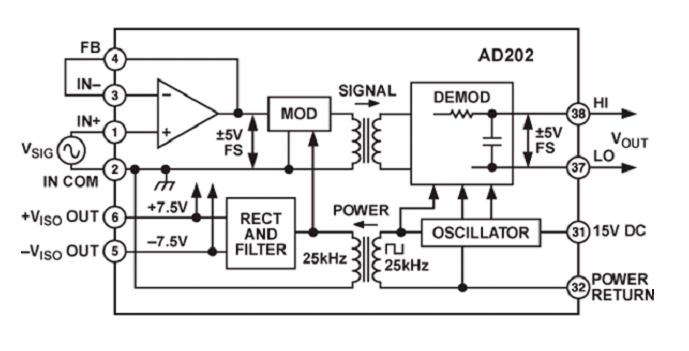
\includegraphics[width=0.8\textwidth]{figuras/AD202-ampop-isolado.png}
    \fonte{\cite{ad202}}
\end{figure}

Esse tipo de amplificador, porém, apresenta alto custo e possui uma variação de leitura considerável com a temperatura. São inferiores em precisão a outros métodos de medição que realizam o isolamento do circuito inerentemente por seus aspectos construtivos.

\subsection{Bobina Rogowski}\label{subsec:Rogowski}

Utilizando-se do princípio da Lei da Indução de Faraday, a bobina Rogowski trata-se de um loop fechado de fio enrolado em volta de um aro. Esse aro envolve o condutor que, por sua variação de corrente, induz uma tensão elétrica proporcional ao número de espiras e a intensidade da própria corrente a ser medida. Para a medida dos valores obtidos pela bobina Rogowski, é necessário o uso de um integrador (por vezes acoplado no próprio cabo da ponteira de medição) para relacionar a derivada da corrente com a tensão obtida em seus terminais, podendo causar certo erro introduzido pela operação.

\begin{figure}[htb!]
    \caption{Bobina Rogowski aberta}
    \label{fig:rogowski-bobina}
    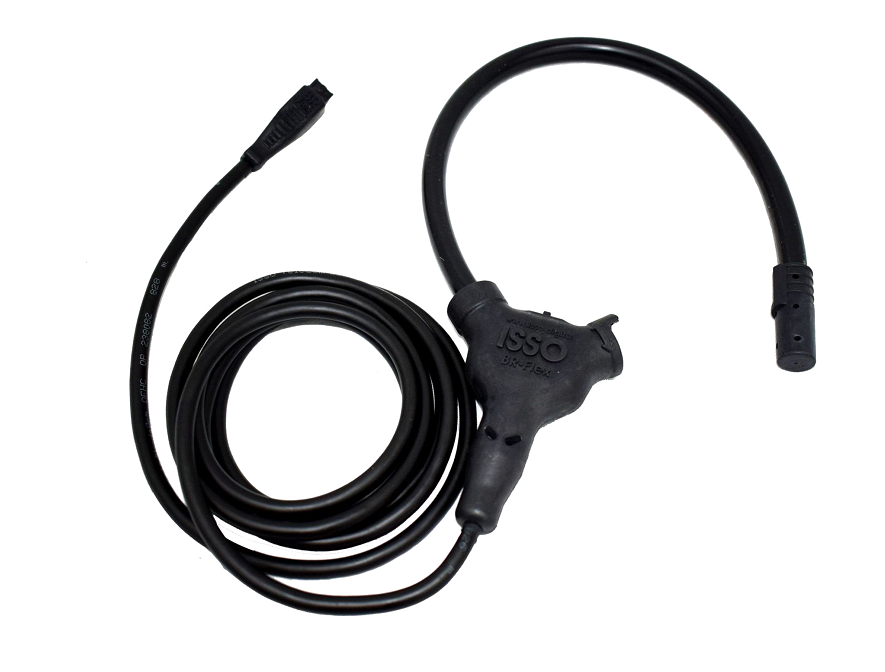
\includegraphics[width=0.8\textwidth]{figuras/bobina-rogowski.png}
    \fonte{\citep{curr_sens_tech}}
\end{figure}

É um método amplamente utilizado para medições de correntes CA elevadas e suporta uma grande faixa de frequências. Tem um custo próximo dos transformadores de corrente e insere menos impedância parasita no circuito \citep{curr_sens_tech}.

\subsection{Circuito Integrado de Medição \textit{(hall effect)}}\label{subsec:halleffect}

Existem circuitos integrados capazes de medir a corrente alternada de maneira isolada do restante do circuito. Utilizando-se do efeito hall, o campo magnético gerado pela corrente que passa entre seus terminais é medida por um sensor montado diretamente no substrato do chip. A saída do CI é uma tensão proporcional ao campo magnético e pode ser medida por um ADC, recuperando-se o valor da corrente original.

O uso dessa tecnologia traz custo baixo em relação ao uso de TC's ou bobinas Rogowski, fácil implementação no sistema, isolamento diretamente no chip. Tal medição, porém, possui uma resolução na ordem de \SI{100}{\milli\volt\per\ampere} (considerando um CI que suporte acima de 10 A) e um ruído intrínseco de 11 mV. Como é o caso do ACS712 \citep{acs712}.

%ADC
\section{Conversor Analógico Digital}\label{sec:ADC}

O \gls{ADC} (\textit{Analog-to-Digital Converter}) é uma parte integral do funcionamento dos equipamentos de medição elétrica, pois este fará o interfaceamento, ou seja, a leitura do sinal analógico a ser interpretado e o converterá para um sinal digital que pode assim ser processado, como mostrado na \autoref{fig:ADCDB}.

\begin{figure}[htb!]%% Ambiente figure
    %\captionsetup{width=0.55\textwidth}%% Largura da legenda
    \caption{Diagrama de blocos de um ADC}%% Legenda
    \label{fig:ADCDB}%% Rótulo
    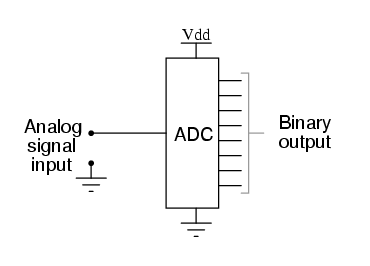
\includegraphics[scale=0.8]{ADCDB}%% Dimensões e localização
    \fonte{\cite{ADCbook}}%% Fonte: Lessons in Electric Circuits: Volume IV - Digital, by Tony R. Kuphaldt
\end{figure}

Existem vários tipos de \gls{ADC}s, sendo alguns deles:

\begin{itemize}
    \item \textit{Flash} \gls{ADC};
    \item \textit{Digital Ramp} \gls{ADC};
    \item \textit{Successive Approximation} \gls{ADC};
    \item \textit{Tracking} \gls{ADC};
    \item \textit{Slope (integrating)} \gls{ADC};
    \item \textit{Delta-Sigma ($\Delta$ $\Sigma$)} \gls{ADC};
    \item entre outros\dots
\end{itemize}

Para fins de objetividade, será somente apresentado o \gls{SAR} (\textit{Successive Approximation Register}), pois este é o mais comumente utilizado em multímetros e o \gls{ADC} mais básico, chamado de \textit{Flash}. Porém, dependendo da aplicação e necessidade de resolução ou precisão, são utilizados outros tipos de \gls{ADC} também.

\subsection{Flash ADC}\label{flashADC}

Este \gls{ADC} delimita o principio de funcionamento desse tipo de dispositivo. Formado de uma série de comparadores, como mostrado na \autoref{fig:flashADC}, este compara o sinal de entrada com uma tensão de referência única para cada comparador. A saída destes comparadores são conectadas à um \textit{encoder} de prioridade que produz uma saída binária.
Esta topologia não só é a mais simples em termos de operação, mas também é o mais eficiente, em termos de velocidade, sendo limitado só pelos comparadores e \textit{delays} de propagação dos gates. Infelizmente, o \textit{flash} \gls{ADC} necessita de um número excessivo de componentes, sendo necessários 255 comparadores para uma saída de 8-bits, que seria a necessidade de \textit{output} de qualquer \gls{ADC} moderno.

\begin{figure}[htb!]%% Ambiente figure
    %\captionsetup{width=0.55\textwidth}%% Largura da legenda
    \caption{Diagrama de blocos de um ADC Flash}%% Legenda
    \label{fig:flashADC}%% Rótulo
    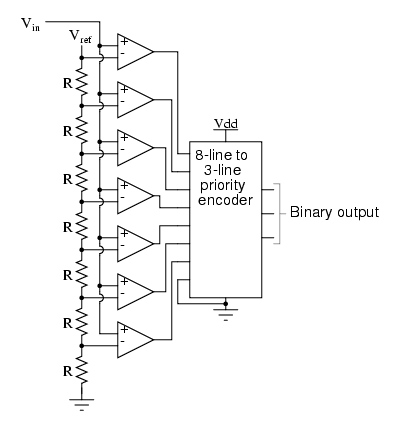
\includegraphics[scale=0.6]{flashADC}%% Dimensões e localização
    \fonte{\cite{ADCbook}}%% Fonte: Lessons in Electric Circuits: Volume IV - Digital, by Tony R. Kuphaldt
\end{figure}

\subsection{SAR ADC}\label{SARADC}
O \gls{SAR} funciona de maneira que se é conectado um contador \gls{SAR}, que faz uma contagem testando todos os valores de bits, começando com o mais significativo e terminando com o menos significativo a um \gls{DAC} que então sua saída é comparada com o sinal analógico a ser obtido.

Durante o processo de contagem, um registro monitora a saída deste comparador para ver se a contagem binária é maior ou menor que a entrada do sinal analógico, ajustando os valores de bit de acordo. A maneira que este registro conta é idêntica ao método de conversão decimal para binário, portanto diferentes valores de bits são testados do bit mais significante ao menos significante para conseguir um número binário que se iguala ao número decimal original.

O circuito e resultado de leitura do \gls{ADC} em questão, em termos simples, pode ser representado pelas figuras \ref{fig:SARADC} e \ref{fig:SARADCplot}.

\begin{figure}[htb!]%% Ambiente figure
    %\captionsetup{width=0.55\textwidth}%% Largura da legenda
    \caption{Diagrama de blocos de um ADC SAR}%% Legenda
    \label{fig:SARADC}%% Rótulo
    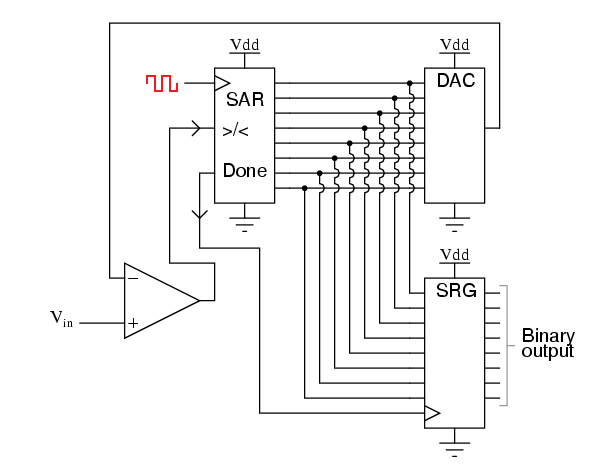
\includegraphics[scale=0.8]{SARADC}%% Dimensões e localização
    \fonte{Adaptado de: \cite{ADCbook}}%% Fonte: Lessons in Electric Circuits: Volume IV - Digital, by Tony R. Kuphaldt
\end{figure}

\begin{figure}[htb!]%% Ambiente figure
    %\captionsetup{width=0.55\textwidth}%% Largura da legenda
    \caption{Plot sobre o tempo da saída de um ADC SAR}%% Legenda
    \label{fig:SARADCplot}%% Rótulo
    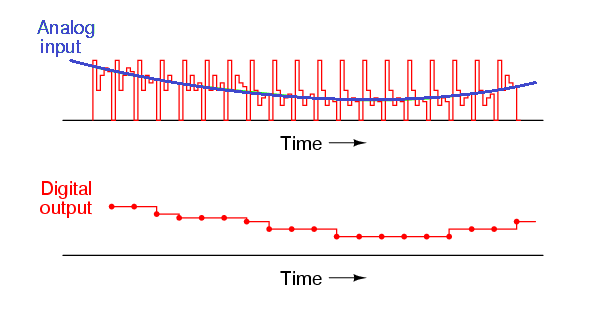
\includegraphics[scale=0.8]{SARADCplot}%% Dimensões e localização
    \fonte{Adaptado de: \cite{ADCbook}}%% Fonte: Lessons in Electric Circuits: Volume IV - Digital, by Tony R. Kuphaldt
\end{figure}

%Referência de tensão
\section{Referência de Tensão}\label{sec:VoltageReference}

A referência de tensão do ADC, utilizada para a leitura do sinal analógico, pode ser interna ou externa ao chip. Quando interna, trata-se de uma solução mais barata e de menor precisão, adequada para equipamentos que não exigem alta precisão. Quando externa, oferece uma melhor precisão e, consequentemente, uma leitura mais precisa. Atualmente, essa referência externa é fornecida por um \gls{CI} (Circuito Integrado) especializado, como o ICL8069 \cite{icl8069}, amplamente utilizado nas soluções mais avançadas.

%input Warning
\section{Aviso de Entrada Incorreta \textit{(Input Warning)}}\label{sec:inpWarning}

O termo \textit{input warning} refere-se a um aviso emitido quando ocorre uma entrada incorreta ou anormal em um sistema de medição. Esse tipo de aviso é acionado quando há um problema que pode afetar a precisão ou a confiabilidade dos dados de medição, como condições fora dos limites esperados, por exemplo, valores de tensão ou corrente que ultrapassam os limites especificados pelo instrumento de medição.

Quando isso ocorre, pode-se utilizar um alarme para alertar o usuário sobre um erro que pode prejudicar a leitura do dispositivo. Os alarmes são divididos em duas categorias principais: \textit{hard} e \textit{soft}.

No caso do alarme \textit{hard}, o aviso é emitido por uma fonte que não depende do circuito, como um relé externo ou um circuito separado de monitoramento. Isso garante que, mesmo que o sistema principal apresente uma falha total, o alerta ainda esteja ativo. No entanto, essa abordagem torna a implementação mais custosa e complexa. Por outro lado, o alarme \textit{soft} provém do próprio circuito e é utilizado como uma forma de alerta quando não há risco direto de falha total do sistema ou quando o alarme é de baixa urgência \cite{base_alarms}.

No contexto do projeto, optou-se pela utilização de um alarme \textit{soft}, uma vez que sua implementação é mais simples — consistindo apenas em um buzzer ligado a uma das portas lógicas disponíveis do microcontrolador — e possui um custo extremamente baixo.

\subsection{Comparador para detecção de falhas} \label{subsec:compfalhas}

Para o caso do multímetro a ser desenvolvido pode-se utilizar um simples circuito comparador para monitorar as tensões de entrada e indicar ao usuário que a escala utilizada está incorreta ou, até mesmo, que a tensão ou corrente medidas está acima do limite suportado. O circuito pode ser visto na \autoref{fig:comparador-simples} e consiste apenas em um \gls{amp-op}.

\begin{figure}[htb!]
    \caption{Circuito de um comparador utilizando dois resistores como referência de tensão}
    \label{fig:comparador-simples}
    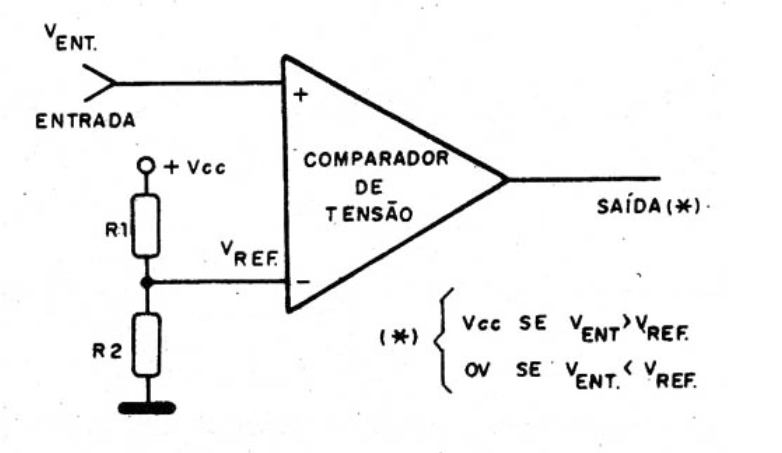
\includegraphics[width=0.8\textwidth]{figuras/ampop-comparador.png}
    \fonte{\cite{comp_ncbraga}}
\end{figure}

Dessa maneira, uma vez definida a tensão de referência, pode-se utilizar-se da saída para disparar algum tipo de aviso.

\subsection{Tipos de aviso} \label{subsec:tiposdeaviso}

Os avisos podem ser luminosos, sonoros ou até mesmo gerar vibrações e movimentações mecânicas mais intensas para alertar ou notificar o usuário sobre o estado do dispositivo \cite{base_alarms}.

Em situações menos graves, como o uso inadequado da escala do medidor, pode-se utilizar uma luz de aviso. Esse tipo de alerta não danifica o dispositivo, mas impede a leitura correta dos dados.

Por outro lado, em casos mais sérios, onde há risco de dano ao aparelho de medição ou até mesmo ao usuário, é necessário um aviso mais contundente, como uma sirene, para garantir a devida atenção \cite{base_alarms}.

\subsection{Alerta durante uso no laboratório} \label{subsec:casosextrgraves}

Um erro comum em laboratórios de eletrônica é a tentativa de medição de tensão elétrica utilizando-se do modo de medição de corrente elétrica do dispositivo.

Comumente a corrente é medida através da queda de tensão em um resistor \textit{shunt}, conforme discorrido em \ref{subsec:resiShunt}. Colocar as ponteiras em um ponto onde haja tensão sem nenhum dispositivo limitador de corrente, faria com que o resistor shunt sofresse um enorme estresse levando possivelmente a sua falha ou diminuição drástica da vida útil.

Como geralmente há um sistema de proteção nesses dispositivos, muitas vezes, há a queima de um elemento fusível no lugar do resistor shunt. Porém, é necessário alertar o usuário de que o uso do equipamento foi incorreto e, caso a corrente seja removida a tempo, preservar a própria proteção. Caso essa seja rompida, também é importante notificar o usuário de que a mesma deve ser substituída.

Para tanto, pode-se utilizar um \textit{buzzer} com o som alto o suficiente para notificar o usuário mesmo em um ambiente com certo ruído, como é o caso de um laboratório de aula.

%MCU/interface
\section{MCU e Interface de Comunicação}\label{sec:MCUInterface}

\subsection{Microcontroladores}\label{subsec:MCU}

O \gls{MCU} ou \textit{Microcontroller Unit} é um dispositivo eletrônico altamente integrado contendo um processador, memória e periféricos de entrada e saída. Os microcontroladores são amplamente utilizados em uma variedade de aplicações, desde eletrodomésticos e automóveis até dispositivos médicos e sistemas de controle industrial.

Ele é projetado para ser compacto, de baixo consumo de energia e fácil de programar. Eles são usados para controlar e executar tarefas específicas em um sistema eletrônico. Ao contrário de um microprocessador, que é projetado para executar uma ampla variedade de tarefas e requer componentes externos adicionais, o \gls{MCU} possui praticamente todos os recursos necessários integrados em um único chip.

No caso dos medidores, o \gls{MCU} é utilizado como o interpretador dos sinais obtidos pelo \gls{ADC}, podendo realizar as operações matemáticas necessárias para se obter os valores médios, eficazes, pico, e demais necessários, a partir da amostragem obtida. Esse é o caso do \textit{3Ph-ozm}, que utiliza um microcontrolador com pré-processador dos dados e como sistema de controle para as funções fundamentais do dispositivo \cite{3ph-ozm}.

Juntamente do \gls{MCU}, o \textit{3Ph-ozm} utiliza um microprocessador para realizar o trabalho de comunicação através de WiFi e Bluetooth.
Tal abordagem, porém, traz um custo mais alto ao projeto, uma vez que um microprocessador é mais caro que um microcontrolador --- que pode ser capaz de tanto processar, como enviar os sinais \cite{uCdiff}.

\subsubsection{Microcontroladores Considerados} \label{subsubsec:uc-disp}

Existe uma vasta gama de \gls{MCU}'s capazes de realizar o processamento dos sinais obtidos. Logo, se faz necessária uma filtragem prévia dos principais requisitos do projeto antes mesmo do inicio da metodologia.
Para tanto, foram considerados os seguintes pontos:

\begin{itemize}
    \item Popularidade --- um item popularmente conhecido pode ser encontrado com maior facilidade em lojas locais;
    \item Facilidade de programação --- como um dos objetivos primordiais do projeto é a replicabilidade e a disponibilização por meios \textit{open source}, a simplicidade na programação deve ser levada em conta;
    \item Preço --- o microcontrolador tem potencial para ser o item único mais custoso do projeto, reduzir seu preço auxiliaria na questão do baixo custo;
    \item Comunicação --- dispositivos com Wifi, \gls{$I^2$C}, UART ou demais protocolos de comunicação já embarcados auxiliariam no processo de transmissão e tratamento dos dados obtidos.
\end{itemize}

Seguindo esses critérios e as informações disponíveis no artigo \textit{How to Select the Microcontroller for Your New Product} \cite{select_uC}, os \gls{MCU}'s adequados à finalidade de medição seriam os que possuem arquitetura de 32 bits, uma vez que estes possuem também certas características de microprocessadores como, por exemplo, a lógica de prioridade nas interrupções e a velocidade de trabalho com ponto flutuante.

Os \gls{MCU}'s mais populares dessa arquitetura são os da família STM32, representado na \autoref{fig:stm32-family}.

\begin{figure}[htb!]
    \caption{Família STM32 separada por função}
    \label{fig:stm32-family}
    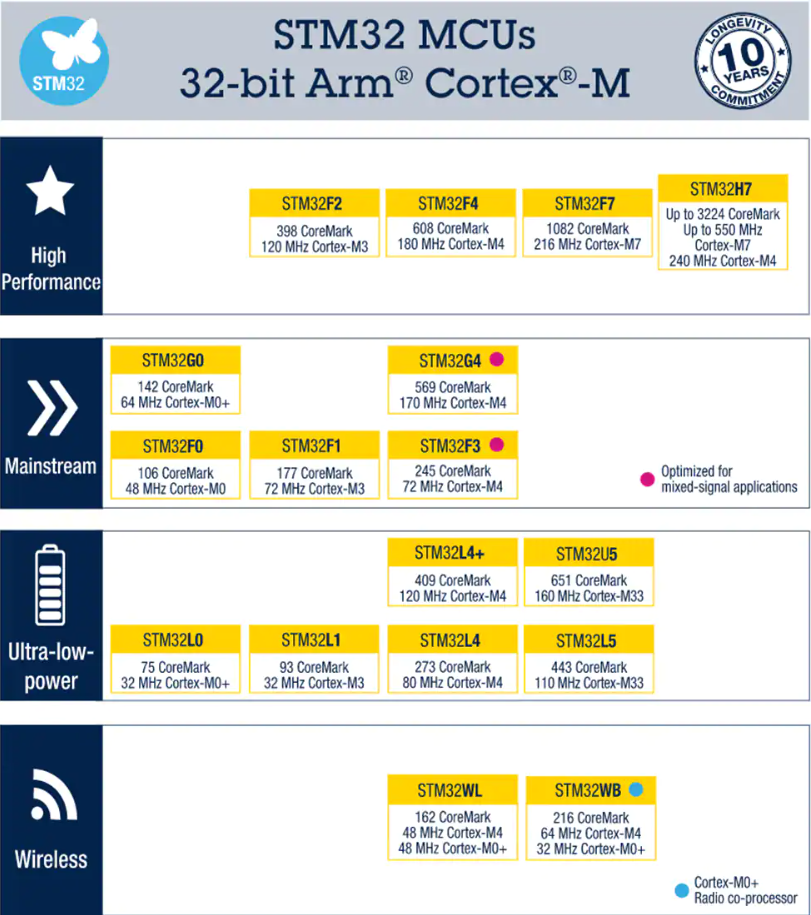
\includegraphics[width=0.7\textwidth]{figuras/STM32-family.png}
    \fonte{Mouser}
\end{figure}

Para a seleção de um microcontrolador adequado, pode-se seguir a linha \textit{mainstream} da \autoref{fig:stm32-family}, pois tratam-se de \gls{MCU}'s populares e que possuem vasta documentação disponível online. Porém, ao utilizar tais microcontroladores, seria necessária a utilização de outro periférico para a função de Wifi e/ou Bluetooth.

\subsection{Apresentação dos dados e Comunicação}\label{sec:Interface}

Os dispositivos de medição que possuem comunicação com sistemas externos o fazem de diversas maneiras.

A mais simples delas trata-se de um display que apresenta os valores da leitura ao usuário. Este pode utilizar a tecnologia de \gls{LCD} ou semelhantes para mostrar apenas números, como também pode mostrar as formas de onda em telas que possuam uma resolução maior.

Os dados também podem ser enviados a um sistema externo que fará a apresentação dos dados, os armazenará para usos posteriores, ou dará outra finalidade conforme o sistema.

Para realizar esse envio, podem-se utilizar diversas tecnologias diferentes, desde protocolos com fio (CAN, MODBUS, \gls{$I^2$C}, UART, etc.) até protocolos sem fio --- que serão os mais aprofundados nessa seção.

Baseando-se no artigo \citet{lowcost-smartmeter}, as tecnologias que podem ser usadas são as encontradas no ambiente de IoT (Internet das Coisas) como LoRa, Sigfox e NB-IoT. Também é possível utilizar tecnologias mais populares, como é o caso do \citet{3ph-ozm} que utiliza WiFi e Bluetooth para realizar sua comunicação e o display de seus dados através de uma interface web conforme a \autoref{fig:interface-3ph-ozm}.

\begin{figure}[htb!]
    \caption{Interface WEB usada no 3Ph-ozm}
    \label{fig:interface-3ph-ozm}
    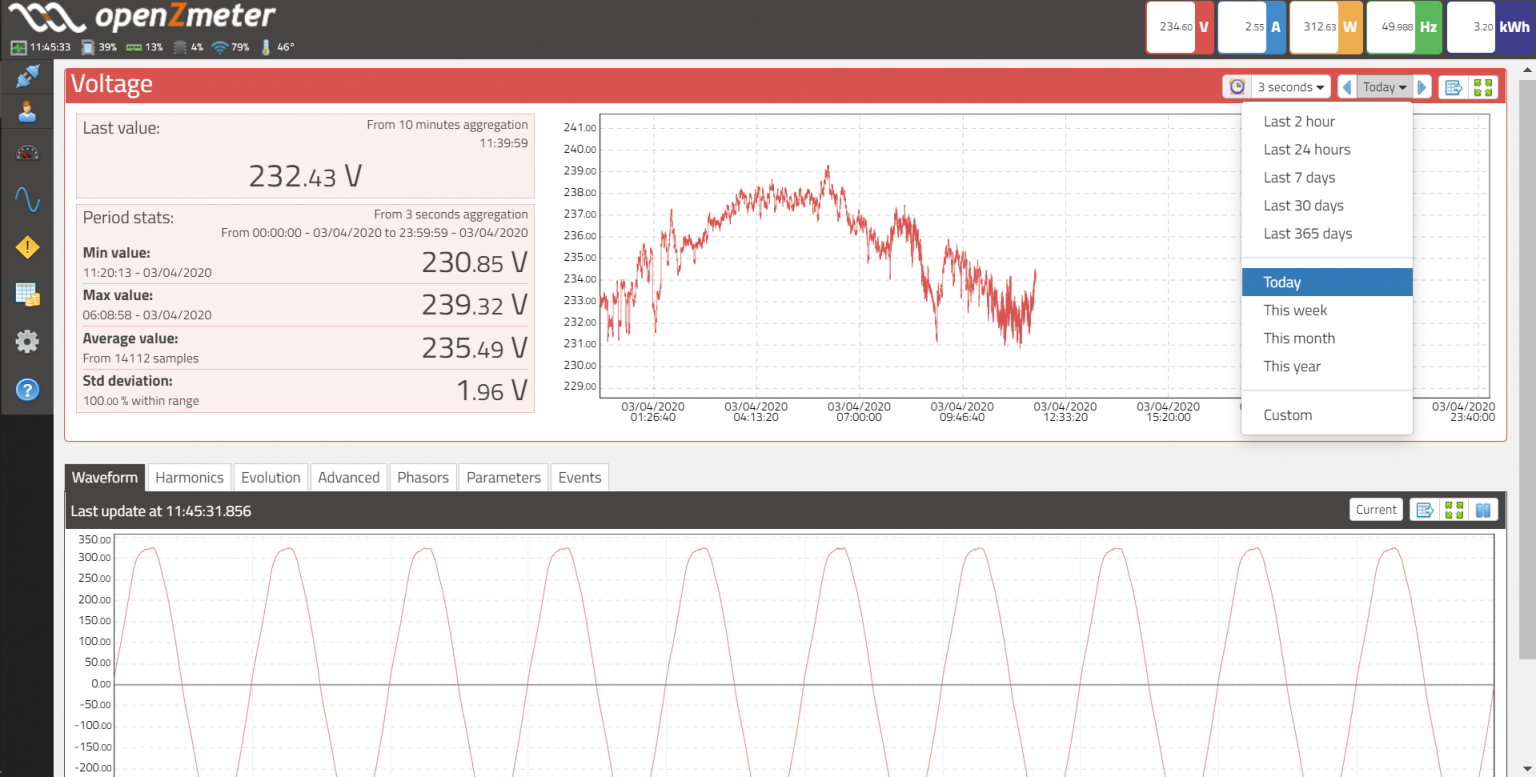
\includegraphics[width=0.9\textwidth]{figuras/interface-web-openzmeter.png}
    \fonte{www.openzmeter.com/}
\end{figure}

\subsection{Soluções completas}\label{subsec:solucomp}

Há também a possibilidade da utilização de módulos que possuem um microcontrolador e outras funções integradas. Como é o caso do ESP32-WROOM-32D (\autoref{fig:esp32-frente-verso}), construído em torno do chip ESP32.

Esse módulo possui um microprocessador \textit{Xtensa® Dual-Core 32-bit LX6} e as funções principais de um microcontrolador, como \gls{ADC} próprio e tratamento de interrupções por ordem de relevância. Além de possuir dois \gls{DAC}'s. O principal diferencial desse módulo, porém, é a sua capacidade de trabalhar com WiFi e Bluetooth sem a necessidade de nenhum periférico extra, além de possuir grande facilidade em sua programação \cite{esp32-datasheet}.

\begin{figure}[htb!]
    \caption{Módulo ESP32-WROOM-32D frente e verso}
    \label{fig:esp32-frente-verso}
    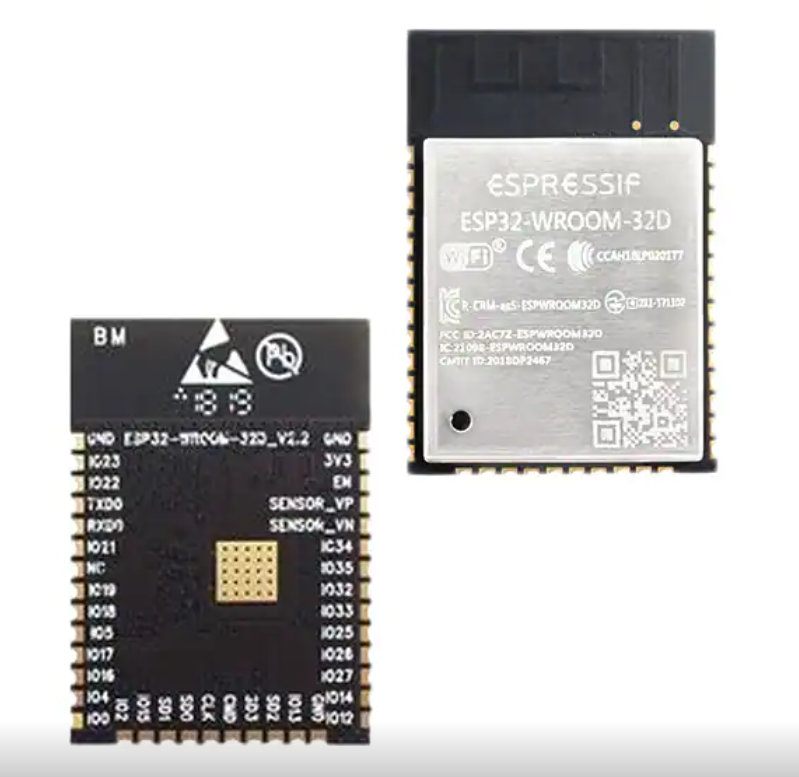
\includegraphics[width=0.3\textwidth]{figuras/esp32-frente-verso.png}
    \fonte{DigiKey}
\end{figure}

%power management
\section{\textit{Power Management}}\label{powerManagement}

Multímetros digitais se apresentam em duas configurações, sendo estas de bancada e portátil. Na configuração portátil, se é utilizado pilhas ou baterias para prover a tensão necessária para se ligar todos os subsistemas do aparelho. Já na configuração de bancada, é utilizada uma fonte isolada, conectada à rede de energia para fornecer a tensão adequada para se ligar todos os subsistemas do dispositivo, como se pode ver nas figuras \ref{fig:bathh} e \ref{fig:batbt}, dos designs propostos pela \gls{TI}.

\begin{figure}[htb!]%% Ambiente figure
    %\captionsetup{width=0.55\textwidth}%% Largura da legenda
    \caption{Diagrama de Blocos de um Multimetro Portátil}%% Legenda
    \label{fig:bathh}%% Rótulo
    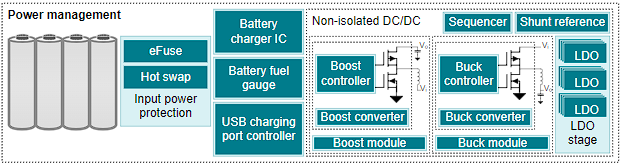
\includegraphics[scale=0.9]{bathh}%% Dimensões e localização
    \fonte{\cite{DMMTI}}%% Fonte
\end{figure}

\begin{figure}[htb!]%% Ambiente figure
    %\captionsetup{width=0.55\textwidth}%% Largura da legenda
    \caption{Diagrama de Blocos de um Multímetro de Bancada}%% Legenda
    \label{fig:batbt}%% Rótulo
    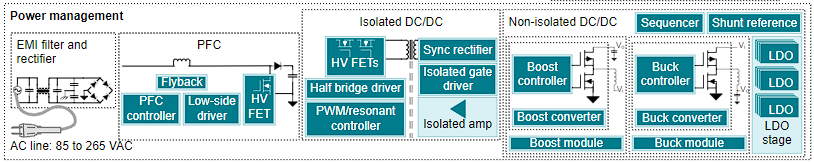
\includegraphics[scale=0.7]{batbt}%% Dimensões e localização
    \fonte{\cite{DMMTI}}%% Fonte
\end{figure}

Existem vários modos de se projetar uma fonte adequada ao sistema proposto, mas para o escopo deste trabalho, foi optado por se utilizar uma fonte comercial que será escolhida para atender as necessidades do protótipo em questão.

%calibração
\section{Calibração}\label{sec:Calibration}

Todo equipamento de medição precisa ser calibrado para exercer a sua função com precisão. Normalmente, este serviço é feito pelo provedor do produto e, dependendo do tipo de uso de tal produto e sua precisão, feito em intervalos regulares para garantir sua eficácia. Muitas vezes, realizar a calibração de um equipamento como um multímetro pode ser mais caro que comprar um novo.

Para se calibrar um multímetro, é utilizado um outro dispositivo com no mínimo 4x a precisão do multímetro a ser calibrado. Portanto, normalmente se é utilizado um equipamento específico para exercer tal função. Esse equipamento geralmente é chamado de \textit{calibrator} ou \textit{standard} \cite{flukecalib}. %ref: https://eu.flukecal.com/products/electrical-calibration-0

Tais equipamentos também necessitam ser calibrados, então o fornecedor deve garantir que estes estejam de acordo com os órgãos regionais, nacionais e internacionais em questão de procedência da calibração. Uma documentação e traçabilidade extensivas são requerimentos indispensáveis.

O \textit{calibrator} tem a capacidade de fornecer sinais elétricos precisos e de função variável, que podem ser produzidos de µV a kV, normalmente. Estes sinais, em ranges específicos, serão lidos pela \gls{UUT} (\textit{Unit Under Test}) e então serão anotados os resultados da medição, fazendo-se um levantamento de dados do multímetro. Após tal levantamento, realiza-se os passos necessários para calibrar tal dispositivo, dependendo das suas necessidades e também do fabricante do mesmo. Este equipamento também consegue fazer medições de precisão, caso seja necessário.

O \textit{standard} cumpre a mesma função do calibrator, mas geralmente é limitado a poucos ranges de geração de sinal e somente uma função, o que possibilita uma performance e precisão muito maior que a do \textit{calibrator}.

Entretanto, existe uma proposta de calibração do equipamento on-board, feita pela \gls{TI} (\textit{Texas Instruments}), utilizando-se um \gls{DAC} para corrigir erros de leitura, seja por mudanças de temperatura, mudança na tensão de referência do \gls{ADC} ou qualquer outro fator que possa afetar a leitura do sinal. Também nesse circuito é incluído um sensor de temperatura para avisar o usuário sobre mudanças consideráveis de temperatura.

O funcionamento do \gls{DAC}, porém, está diretamente relacionado à sua tensão de referência. Geralmente, se é utilizada uma referência externa para medidas de precisão, pois esta estará isolada da aquisição de sinal do multímetro e logo não será afetada caso haja uma mudança de temperatura \cite{analogdac}. A solução proposta pela \gls{TI} é de se utilizar um \gls{DAC} de precisão (16-Bits) com \textit{on-board low-drift voltage reference} junto com um \textit{buffer} por meio de um \gls{amp-op} de alta velocidade. Tais componentes são de uso extremamente específico e por isso são caros, colocando-os assim fora do escopo do estudo deste trabalho \cite{DACTI}. %ref: https://www.analog.com/en/analog-dialogue/articles/buffering-the-output-of-high-speed-dacs.html e https://www.ti.com/lit/ug/tiduct8/tiduct8.pdf?ts=1685988821918&ref_url=https%253A%252F%252Fwww.ti.com%252Fsolution%252Fdigital-multimeter-dmm%253Fvariantid%253D20220%2526subsystemid%253D33430

%% Comente para remover este item

%% Capítulo
\chapter{Especificações e Premissas Adotadas}\label{cap:especificacoes}

Neste capítulo, serão apresentadas tanto as especificações do protótipo quanto as premissas adotadas, tendo em vista os objetivos do projeto.

\section{Especificações}\label{spec}
Baseado em relatos dos professores das disciplinas de Fenômenos Eletromagnéticos e Análise de Circuitos A e B da \gls{utfpr} de Curitiba, os equipamentos utilizados nos laboratórios destas disciplinas, bem como os utilizados no \gls{SEMAP} (Setor de Almoxarifado/Manutenção dos Laboratórios) da universidade, definiram-se as seguintes especificações elétricas para o multímetro desenvolvido, conforme a \autoref{tab:specstable}:

\begin{table}[!ht]
    \centering
    \caption{Resolução e precisão necessárias para o dispositivo}
    \label{tab:specstable}
    \begin{tabular}{ l l l }
        \hline
        \textbf{Especificação}    & \textbf{Tensão} & \textbf{Corrente} \\ \hline
        \textbf{Faixa de Leitura} & 0 - 220V        & 0 - 10 A          \\ 
        \textbf{Precisão}         & <2\%            & <5\%              \\ \hline
    \end{tabular}
    \fonte{}
\end{table}

Foram também definidas as especificações quanto a construção e sistemas do dispositivo, conforme segue:

\begin{itemize}
    \item Número de bornes para tensão: 2
    \item Número de bornes para corrente: 2
    \item Tipo de alimentação: Fonte interna isolada
    \item Display de dados: \textit{Smartphones} com acesso a navegador, por \textit{Wi-Fi}.
\end{itemize}

Os dados que o dispositivo será capaz de apresentar ao usuário são:

\begin{itemize}
    \item Formas de onda de tensão e corrente simultâneas,
    \item Tensão e corrente RMS,
    \item Potência ativa, reativa, aparente,
    \item Fator de potência.
\end{itemize}

\section{Premissas Adotadas}\label{premissas1}

As premissas deste trabalho são de suma importância, visto que o objetivo do mesmo é projetar um protótipo com um alto nível de replicabilidade e sendo o mais barato possível. Para isso, serão utilizadas as plataformas gratuitas descritas em seguida e também será fornecido um \textit{link} para o repositório no qual será desenvolvido o software.

\subsection{\textit{Hardware}}\label{proto}

Primeiramente, nota-se que o circuito e a \textit{\gls{PCB}} estão sendo desenvolvidos em uma plataforma chamada easyEDA. Esta plataforma, além de fornecer todo um sistema para simulações e desenvolvimento, possúi uma \textit{supply chain} integrada, tornando extremamente simplificado o desenvolvimento e a prototipagem do circuito, sendo possível escolher já as \textit{footprints} de todos os componentes e também já verificar a disponibilidade destes no mercado.

O roteamento das trilhas de cobre, definição de sua espessura e também o a modelagem em 3D da \textit{\gls{PCB}} são disponíveis nesta plataforma, tornando-a extremamente versátil. Tudo isto é fornecido de forma gratuita pelo site.

Assim, além de ser desenvolvido em uma plataforma gratuita, o projeto desenvolvido será disponibilizado para acesso pelo \textit{link} disponibilizado no final deste trabalho.

\subsection{Software e Firmware}\label{softw}

O desenvolvimento completo do \textit{software} utilizado neste projeto se dá pelo editor de código chamado \textit{Visual Studio Code}, ou em abreviação, \gls{VSCode}. Esta plataforma é gratuita e oferece suporte para todas as linguagens de programação.

Dentro deste editor, existem 3 vetores de programação que serão a base do \textit{software} e \textit{firmware}. Primeiramente, se é utilizado \gls{HTML} 5 e \gls{JS} (JavaScript) para a construção do aplicativo web que servirá de monitor para os dados obtidos pelos sensores.

Para o código em Arduino que controlará o ESP32 e também o \textit{Firmware}, será utilizado o PlatformIO, uma \textit{\gls{IDE}} (\textit{Integrated Development Environment}) gratuita que é uma extensão do VSCode.

Por último, será utilizado o \gls{Git}, que é um software de controle e versionamento de código, tornando assim possível a disponibilização de todo o software desenvolvido neste projeto e também seu versionamento por meio de um site chamado \gls{GitHub}. Tal software também pode ser utilizado como uma extensão do VSCode, aumentando e simplificando ainda mais a disponibilidade do software desenvolvido. O \textit{link} para o repositório está disponibilizado no final deste trabalho.





%% Capítulo
% % ATENÇÃO - veja com o seu orientador se você vai ter este capítulo e se este vai ter nome!
\chapter{Trabalhos Relacionados}
\label{cap:trabalhos:relacionados}

Apresente aqui os trabalhos similares ao seu trabalho ou que são importantes para o entendimento do seu trabalho...

(ATENÇÃO - )
\caixa{Atenção}{Veja com o seu orientador se você vai ter este capítulo e se este vai ter nome, talvez ele seja uma seção de outro capítulo...}


TEXTO TEXTO TEXTO TEXTO TEXTO TEXTO TEXTO TEXTO TEXTO TEXTO TEXTO TEXTO TEXTO TEXTO TEXTO TEXTO TEXTO TEXTO TEXTO TEXTO TEXTO TEXTO TEXTO TEXTO TEXTO TEXTO TEXTO TEXTO TEXTO TEXTO TEXTO TEXTO TEXTO TEXTO TEXTO TEXTO TEXTO TEXTO TEXTO TEXTO TEXTO TEXTO TEXTO TEXTO TEXTO TEXTO TEXTO TEXTO TEXTO TEXTO TEXTO TEXTO TEXTO TEXTO TEXTO TEXTO TEXTO TEXTO TEXTO TEXTO TEXTO TEXTO TEXTO TEXTO TEXTO TEXTO TEXTO TEXTO TEXTO TEXTO TEXTO TEXTO TEXTO TEXTO TEXTO TEXTO TEXTO TEXTO TEXTO TEXTO TEXTO TEXTO TEXTO TEXTO TEXTO TEXTO TEXTO TEXTO TEXTO TEXTO TEXTO TEXTO TEXTO TEXTO TEXTO TEXTO TEXTO TEXTO TEXTO TEXTO TEXTO TEXTO TEXTO TEXTO TEXTO TEXTO TEXTO TEXTO TEXTO TEXTO TEXTO TEXTO TEXTO TEXTO TEXTO TEXTO TEXTO TEXTO TEXTO TEXTO TEXTO TEXTO TEXTO TEXTO TEXTO TEXTO TEXTO TEXTO TEXTO TEXTO TEXTO TEXTO

%---------------------------------------------------%

%% Comente para remover este item

%% Capítulo
% \include{./capitulos/cap-proposta}%% Comente para remover este item

%% Capítulo
%%%% CAPÍTULO 3 - MATERIAL E MÉTODOS (PODE SER OUTRO TÍTULO DE ACORDO COM O TRABALHO REALIZADO)

\chapter{Materiais e Metodologia}\label{cap:materialemetodos}

Neste capítulo, serão discutidos e analisados todos os processos relacionados com o desenvolvimento do protótipo, a justificativa de cada escolha tomada, assim como um \textit{\gls{BOM}} (\textit{Bill of Materials}) consolidado, com os preços na data do trabalho, para a confecção de um protótipo.


\section{Metodologia}\label{sec:metodo}

Esta seção será dedicada à discussão sobre todas as partes integrantes do protótipo.

\subsection{Circuito}\label{circuit}

O circuito foi projetado para seguir um fluxo de informações conforme o diagrama de blocos representado na \autoref{fig:dflux}. Baseando-se na pesquisa apresentada no \autoref{cap:referencialTeorico}, este fluxo foi feito para guiar a lógica de design e também para explicar sucintamente o que cada parte do sistema compreende.

\begin{figure}[htb!]
    \caption{Diagrama de Blocos da Lógica de Funcionamento}
    \label{fig:dflux}
    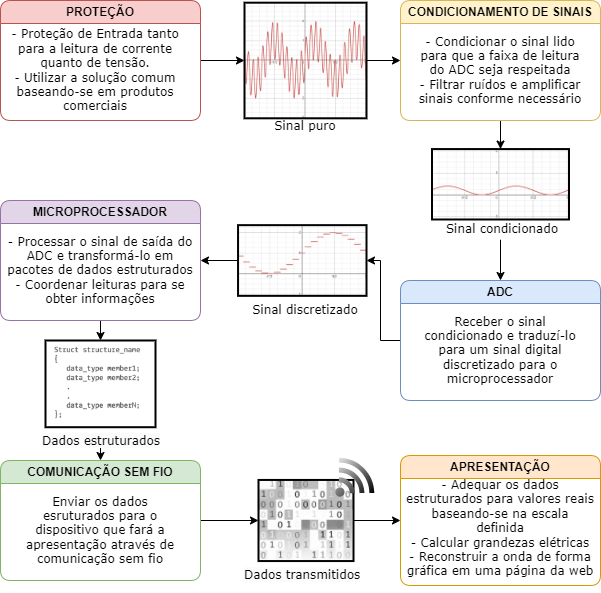
\includegraphics[width=1.0\textwidth]{figuras/dblocflux.png}
    \fonte{}
\end{figure}

Primeiramente, se tem a proteção de entrada. Esta é dividida em duas partes, sendo uma delas a proteção da entrada da tensão e a outra da corrente. Para se proteger a entrada de tensão, utilizam-se um resistor \gls{PTC} e \gls{MOV}s. O \gls{PTC} é projetado para caso a tensão de entrada do circuito seja muito maior que a desejada ou tenha um curto, este esquente e vire uma impedância muito grande, sendo assim uma barreira para qualquer tipo de corrente. Porém, a sua atuação para proteção é demasiada lenta, se pondo necessário a implementação dos \gls{MOV}s, que atuarão mais rapidamente e fecharão um curto entre a entrada e o ground do circuito enquanto o resistor está sendo ativado.

Para a proteção de corrente, utiliza-se primeiramente fusíveis \gls{HRC}, que são fusíveis especiais projetados para extinguir qualquer possível arco voltaico resultante da queima do filamento interno. Isso evita a continuidade da corrente após a atuação do fusível.

Em seguida, a ponte de diodos, posicionada logo após os resistores shunt, atua como um limitador de tensão (clamp) para evitar que a tensão ultrapasse os valores desejados. Além disso, ela proporciona um caminho para a corrente quando esta não é suficiente para queimar os fusíveis, mas pode danificar o circuito.

A disposição desses componentes e sua montagem estão detalhadas na \autoref{fig:circ-prot}.

\begin{figure}[htb!]
    \caption{Entrada de Tensão e Corrente}
    \label{fig:circ-prot}
    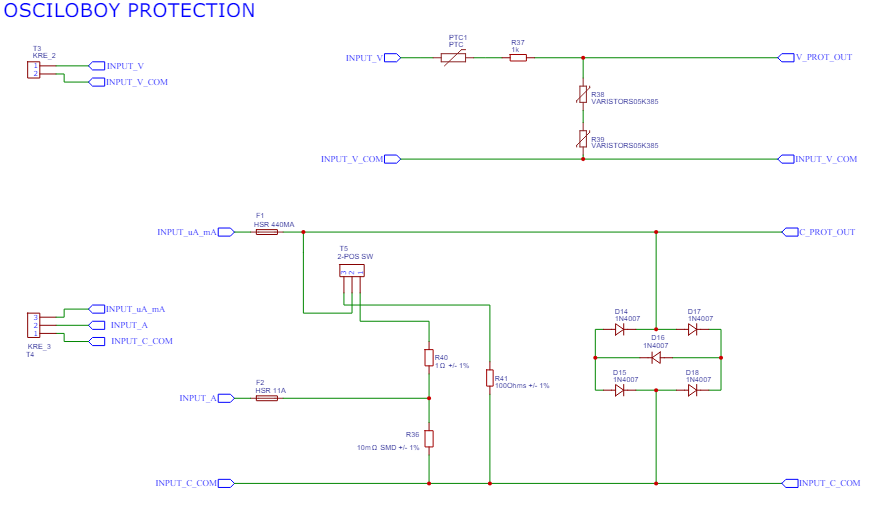
\includegraphics[width=1.0\textwidth]{figuras/circ-prot.png}
    \fonte{}
\end{figure}

Nesta figura, também é possível observar as entradas do circuito. A entrada de tensão está diretamente conectada à próxima etapa, responsável pelo condicionamento dos sinais de tensão. Já a entrada de corrente é composta por resistores que atuam como shunts (R41, R36 e R41), permitindo a leitura da corrente.

O resistor de 10 m$\Omega$ é para a leitura de corrente na proporção de Amperes, a série entre este e o resistor de 1 $\Omega$ compõe a leitura da entrada de mA e o resistor de 100 $\Omega$ para a leitura de $\mu$A. Para alternar entre as entradas de mA/$\mu$A e A, foi colocada uma chave mecânica de duas posições.

Para se obter um sinal apropriado para o ADC, existem duas possibilidades: leitura "Diferencial" e leitura "\textit{Single-Ended}".

\subsubsection{Modo \textit{Single-Ended}}\label{single-ended}

A primeira opção a ser considerada foi a \textit{Single-Ended}. Este tipo de leitura é feita pela comparação de tensão entre um ponto do circuito e o \textit{ground}. Para fazer tal leitura com diferentes \textit{ranges}, o que é fundamental para se alcançar uma boa precisão, foi primeiro projetado um condicionamento de sinais por divisor resistivo, como representado na \autoref{fig:div-res}.

\begin{figure}[htb!]
    \caption{Condicionamento de sinais por divisor resistivo para leitura \textit{Single-Ended}}
    \label{fig:div-res}
    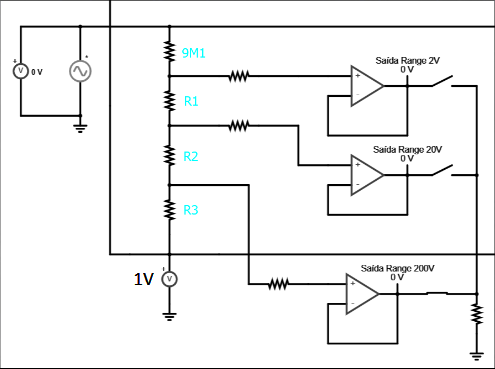
\includegraphics[width=0.6\textwidth]{figuras/div-res.png}
    \fonte{}
\end{figure}

Esta topologia promete 4 ranges de leitura tanto para corrente quanto para tensão, sendo estes 200 V, 20 V, 2 V e 200 mV e 10 A, 200 mA, 20 mA e 2000 $\mu$A. É também necessário o uso de \gls{amp-op}s para a seleção do range, para isolar o \gls{ADC} da entrada e também para manter a tensão de entrada do \gls{ADC} dentro do range requerido.

Desta maneira, foram calculados os resistores de forma a manter a tensão de entrada dos \gls{amp-op}s sempre entre 30 e -30 V no maior fundo de escala possível (atenuação de 10x), respeitando os aspectos construtivos destes componentes. Fixando-se o resistor de entrada como 9,1 M$\Omega$, o cálculo para os demais resistores se resume na resolução do seguinte sistema:

\begin{equation}
    \label{eq01}
    \left\{\begin{matrix}
        \\ \frac{300}{9100000+x+y+z} = i
        \\ \frac{20}{9100000+x+y+z} = j
        \\ \frac{200}{9100000+x+y+z} = k
        \\ i (x+y+z) = 30
        \\ kz = 1
        \\ j(y+z) = 1
    \end{matrix}\right.
\end{equation}

Obtendo os resultados de $x = 5,505556 \cdot 10^{5}, y = 4,55 \cdot 10^{5}$ e $z = 50555,6$, sendo escolhidos os valores comerciais mais próximos.

Substituindo x, y e z, respectivamente, em R1, R2 e R3 na \autoref{fig:div-res}, chega-se às tensões condicionadas desejadas. Com isto, agora, é necessário serem respeitadas as necessidades do \gls{ADC}, que é o componente principal do circuito, pois este efetivamente fará as leituras.

Primeiramente, foi escolhido o \gls{ADC} ADS1115 da \textit{Texas Instruments}, pois este possui 16-bits de resolução, o que torna a leitura extremamente precisa. Possui uma referência interna de tensão, sendo desnecessária a construção de uma referência no circuito, tornando-o menos complexo, e compatível com o protocolo de comunicação \gls{$I^2$C} que será utilizado para interfacear este com o microcontrolador. Porém, devido a sua taxa de leitura extremamente baixa, de 860 \textit{samples per second} (\gls{SPS}), prejudicando a leitura até de frequências na faixa de 60 Hz, foi decidido se utilizar o \gls{ADC} ADS1015.

Este, também da \gls{TI}, apesar de ter uma resolução mais baixa de 12-bits, oferece uma taxa de 3300 \gls{SPS}, possibilitando assim uma reconstrução mais fiel da onda a ser lida, possuindo, uma referência interna de tensão e compatibilidade com o protocolo \gls{$I^2$C}. Este \gls{ADC} também possui uma proteção interna contra surtos por \gls{TVS}, tornando-o extremamente robusto. Os requerimentos para o funcionamento adequado deste \gls{ADC} são uma tensão de entrada máxima de 3,3 V e esta não pode ser negativa.

Seguindo esses parâmetros, percebe-se que o condicionamento de sinal é inadequado, exigindo mais componentes e circuitos auxiliares para funcionar corretamente. Para garantir a leitura de tensões negativas, limita-se a tensão de entrada a um intervalo entre -1 V e 1 V, adicionando um offset de 1 V. Dessa forma, sinais entre 0 V e 1 V são interpretados como negativos, enquanto sinais entre 1 V e 2 V são interpretados como positivos.

Na leitura \textit{Single-Ended}, após o divisor resistivo e o primeiro buffer, é necessário inverter o sinal de saída do \gls{amp-op}. Para isso, utiliza-se um amplificador operacional em cascata, que inverte o sinal de entrada. Além disso, para que esses componentes suportem tensões negativas, é fundamental que a alimentação do circuito seja simétrica, o que requer a inclusão de um circuito auxiliar chamado \textit{Negative Charge Pump}, capaz de fornecer essa tensão negativa.

Outro ponto crucial é que o offset de tensão precisa ser extremamente preciso para minimizar erros na leitura do sinal. Existem \gls{CI}s que oferecem essa precisão, mas eles são bastante caros.

Por fim, para sinais com menor amplitude, é necessário adicionar mais um amplificador operacional em cascata para amplificar o sinal, uma vez que ele estaria fora do alcance do bit menos significativo do \gls{ADC}. O circuito de condicionamento de sinais resultante pode ser visto na \autoref{fig:cascata}.

\begin{figure}[htb!]
    \caption{Condicionamento de sinais por divisor resistivo para leitura \textit{Single-Ended}, menor range}
    \label{fig:cascata}
    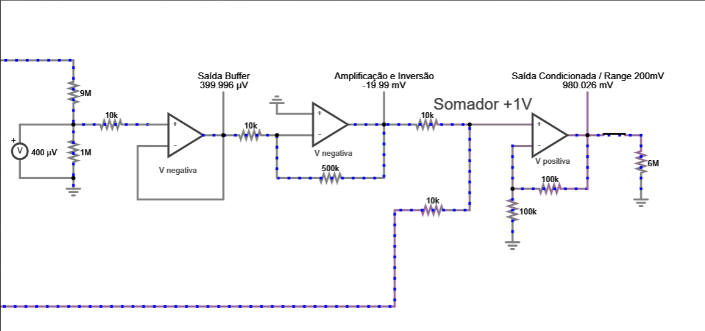
\includegraphics[width=0.8\textwidth]{figuras/cascata.png}
    \fonte{}
\end{figure}

Cada amplificador operacional (amp-op) possui um \textit{drift} de saída, o que introduz ainda mais erro na leitura do \gls{ADC}. Além disso, como é necessária uma amplificação final do sinal, quaisquer ruídos introduzidos também serão amplificados. Com esses problemas combinados, decidiu-se realizar a leitura no modo diferencial, que é a outra opção de leitura nativa disponível no \gls{ADC} escolhido.

\subsubsection{Modo Diferencial}\label{modo-diferencial}

Este tipo de leitura, ao invés de comparar a tensão entre um ponto do circuito e o \textit{ground}, compara a tensão entre dois pontos do circuito e mede efetivamente a diferença entre elas, como mostrado na \autoref{fig:difread}. Isso significa que nenhuma das entradas está ligada a uma referência, eliminando assim problemas referentes ao isolamento da leitura com o terra e também eliminando ruídos de entrada, pois como estes são introduzidos dos dois lados, eles se cancelam.

\begin{figure}[htb!]
    \caption{Condicionamento de sinais por divisor resistivo para leitura diferencial}
    \label{fig:difread}
    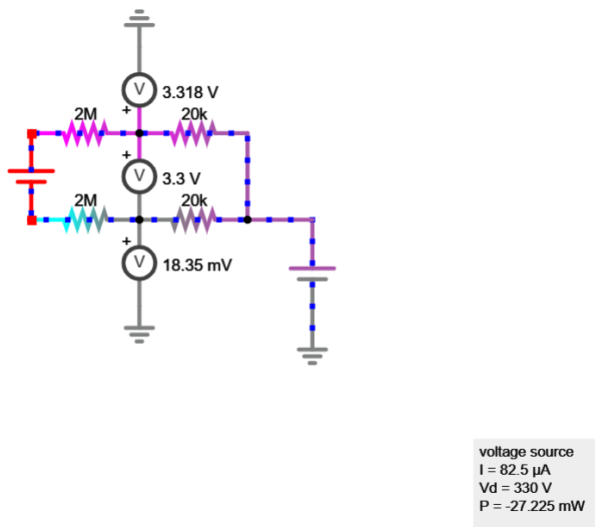
\includegraphics[width=0.6\textwidth]{figuras/difread.png}
    \fonte{}
\end{figure}

Para o dimensionamento dos resistores desta topologia, é necessário atenuar a tensão em aproximadamente 100 vezes, uma vez que um sinal de 330 V (o pico máximo suportado pelo sistema) deve ser condicionado para, no máximo, 3,3 V. Considerando o divisor resistivo, essa atenuação requer uma relação de cerca de 100 vezes entre os resistores. Para garantir uma corrente mínima de entrada, foi escolhido um resistor de 2 M$\Omega$, o que define o segundo valor em 20 k$\Omega$.

Para o offset de tensão, como os erros introduzidos são minimizados pela própria topologia, utiliza-se uma referência de tensão menos precisa, diminuindo o custo do circuito regulador como um todo. A referência de tensão utilizada para este projeto é fornecida pelo \gls{CI} TL431A, tendo este ainda assim uma precisão de 1\%, mas sendo muito mais barato que a opção anterior. Além disso, este possibilita a utilização do range inteiro de leitura do \gls{ADC}, sendo necessário apenas um offset de $3,3/2 V$, utilizado para garantir que as entradas do ADC não recebam tensões negativas, e que pode ser regulado pela ação do \textit{trimpot} junto ao circuito auxiliar. Como não são utilizados \gls{amp-op}s, também não é necessária a utilização do circuito auxiliar \textit{Negative Charge Pump}.

Então, com todos estes benefícios em mente, foi escolhida esta topologia e tipo de leitura para o circuito final, como explícito na \autoref{fig:circ-cond-t}. Para a leitura de corrente, a mesma lógica se aplica, pois o resistor shunt é visto como uma fonte de tensão pelo circuito de leitura. Como esta tensão é extremamente baixa, não há a necessidade de um resistor de entrada para a atenuação da mesma, como explícito na \autoref{fig:circ-cond-c}.

\begin{figure}[htb!]
    \caption{Circuito de condicionamento de sinais para tensão}
    \label{fig:circ-cond-t}
    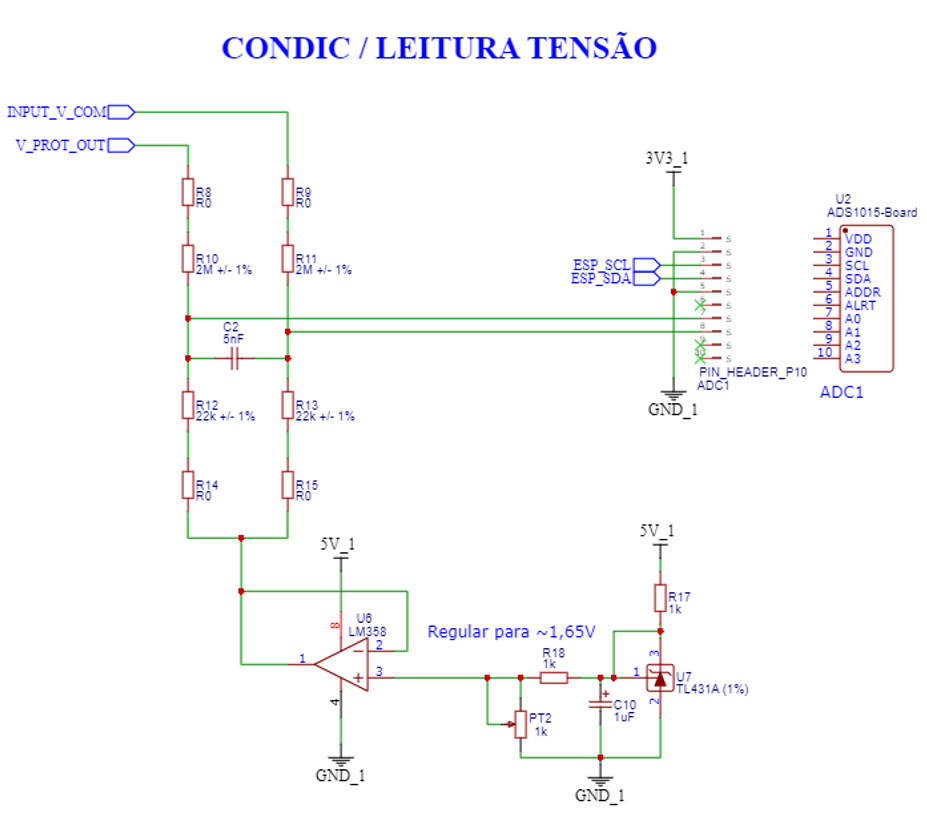
\includegraphics[width=0.8\textwidth]{figuras/circ-cond-t.png}
    \fonte{}
\end{figure}

\begin{figure}[htb!]
    \caption{Circuito de condicionamento de sinais para corrente}
    \label{fig:circ-cond-c}
    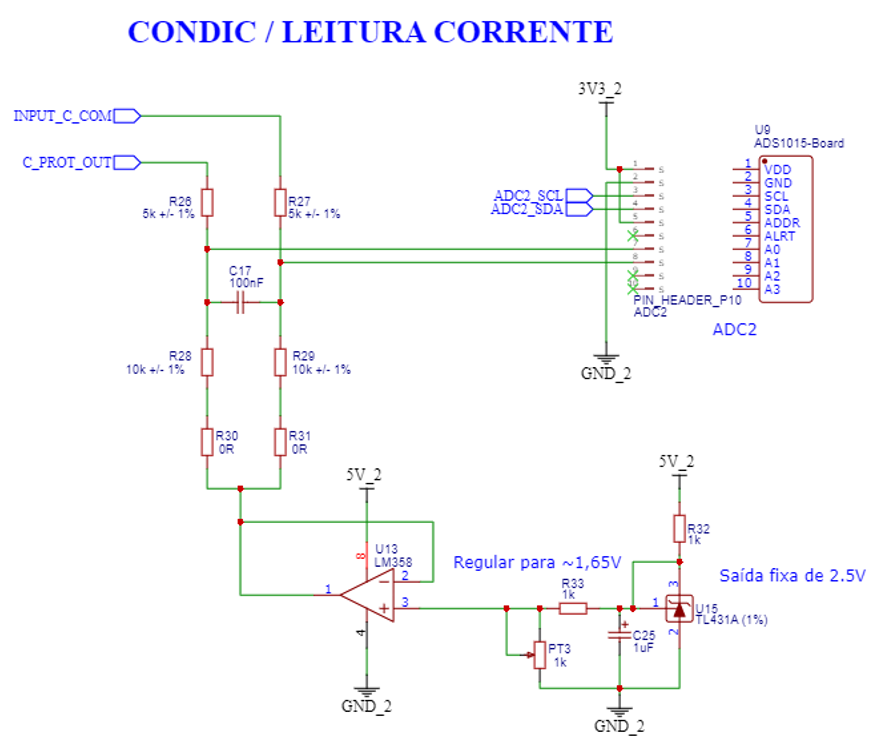
\includegraphics[width=0.8\textwidth]{figuras/circ-cond-c.png}
    \fonte{}
\end{figure}

Também sobre o condicionamento de sinais, é de suma importância se ter um filtro de entrada. Mesmo que a topologia em questão minimize ruídos, quanto mais limpo o sinal de entrada é, melhor serão as leituras e consequentemente o tratamento dos dados. Para este projeto, decidiu-se utilizar um filtro passa-baixas "RC", que consiste de um resistor e um capacitor em \textit{shunt} \cite{filtros}. O cálculo deste filtro é regido pela fórmula \autoref{eqcap}:

\begin{equation}
    \label{eqcap}
    f_{c} = \frac{1}{2\pi RC}
\end{equation}

Este filtro age de forma a atenuar em \textit{3dB} (70,7\%) sinais de frequências maiores que a de corte.

Para o cálculo deste filtro, precisa-se encontrar o R equivalente nos nós do capacitor. Para tanto, utiliza-se o teorema de Thevenin (considerando todas as fontes de corrente como circuito aberto e fontes de tensão como curto), como é possível verificar substituindo o capacitor por um ohmímetro na \autoref{fig:r-thevenin}.

\begin{figure}[htb!]
    \caption{Simulação da resistência de Thevenin}
    \label{fig:r-thevenin}
    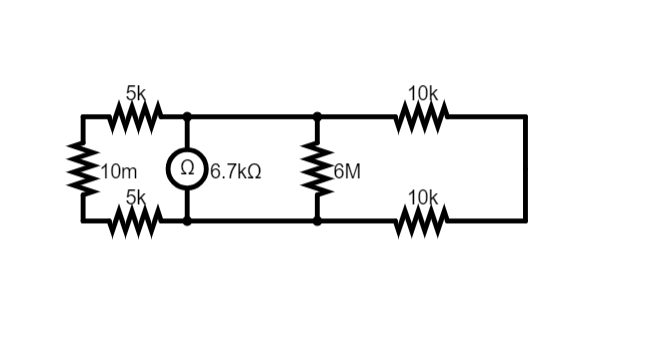
\includegraphics[width=0.9\textwidth]{figuras/r-thevenin.png}
    \fonte{}
\end{figure}

Utilizando a fórmula, para o caso da entrada de corrente e considerando dois resistores de 5 k$\Omega$ (pela facilidade de se encontrar o componente), chega-se ao valor de um capacitor de aproximadamente 100 nF para uma frequência de corte de aproximadamente 237 \textit{Hz}. As simulações representadas nas figuras \ref{fig:simco1} e \ref{fig:simco2}. O sinal encontrado no resistor de 6 M$\Omega$ representa a entrada do \gls{ADC}.

\begin{figure}[htb!]
    \caption{Simulação sem filtro passa-baixa para a corrente}
    \label{fig:simco1}
    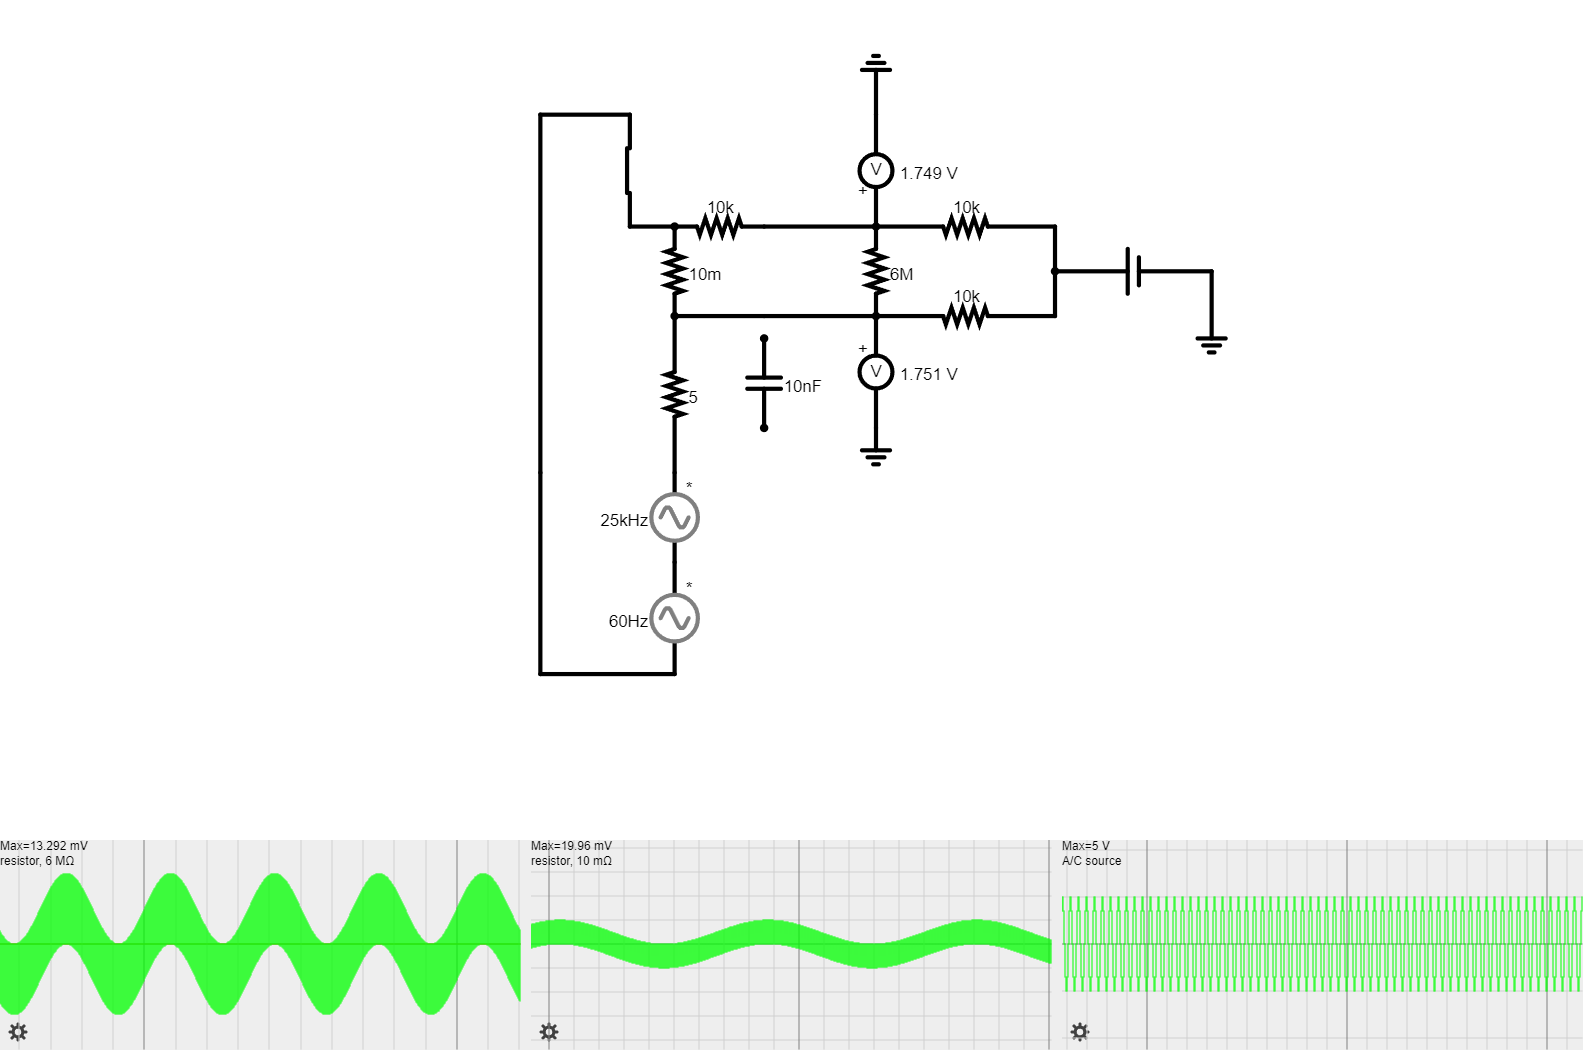
\includegraphics[width=0.9\textwidth]{figuras/sim-co-1.png}
    \fonte{}
\end{figure}

\begin{figure}[htb!]
    \caption{Simulação com filtro passa-baixa para a corrente}
    \label{fig:simco2}
    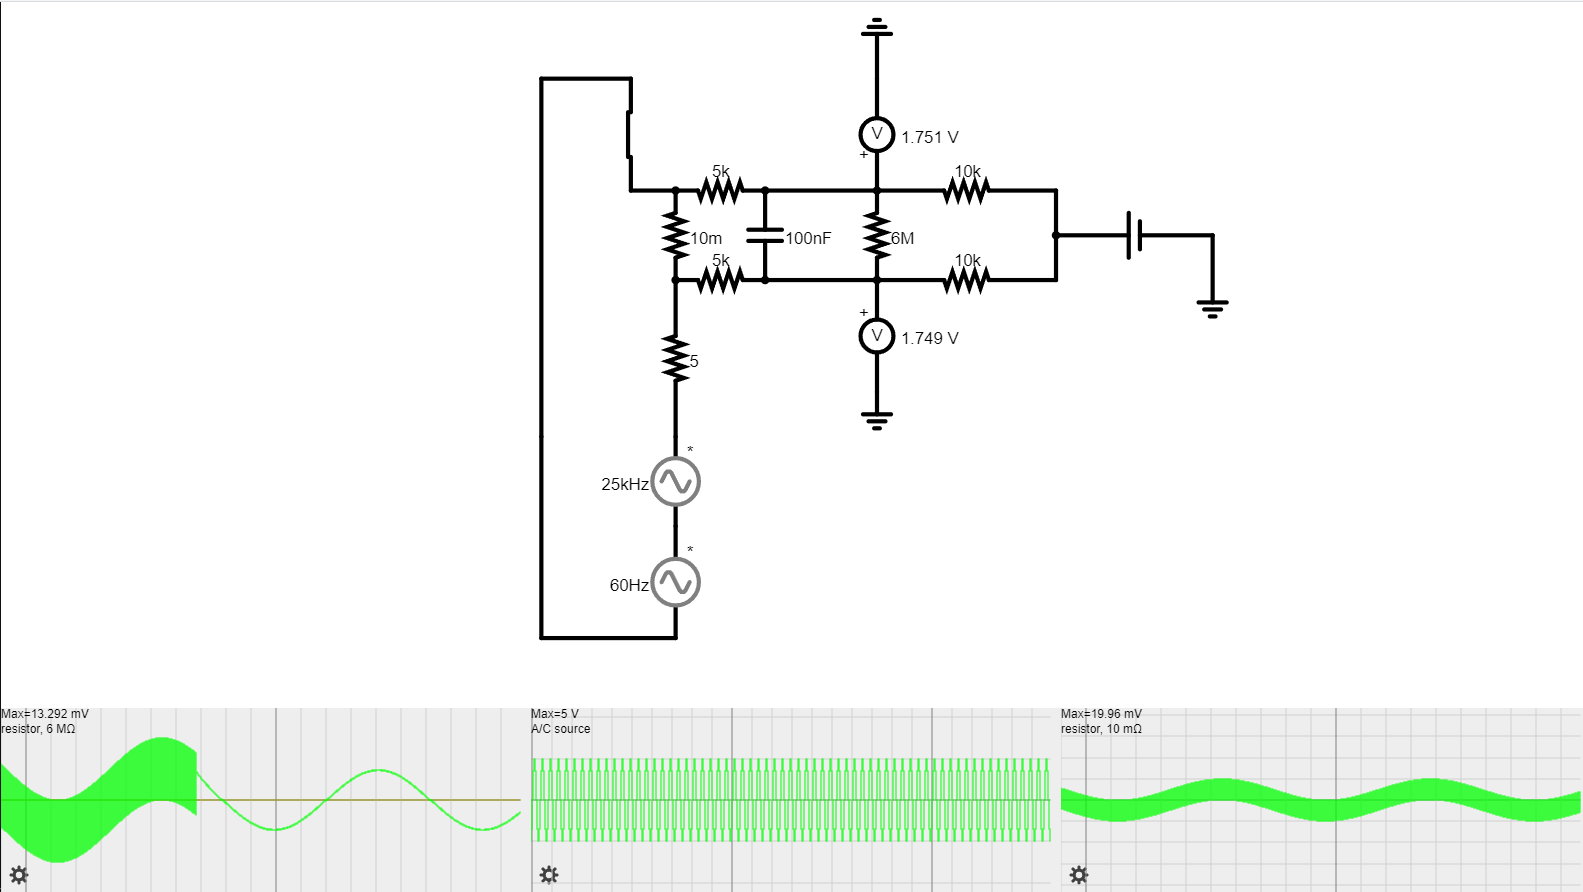
\includegraphics[width=0.9\textwidth]{figuras/sim-co-2.png}
    \fonte{}
\end{figure}

Para a entrada de tensão do circuito segue-se a mesma lógica, chegando a um valor de aproximadamente 5 nF.

Após a leitura dos sinais e a conversão feita pelo ADC, o sinal digital de saída é processado por um microcontrolador para então ser entregue a uma webpage e assim tratado para visualização pelo usuário. Algumas necessidades básicas devem ser atendidas pelo chip escolhido, como suporte para comunicação \textit{wireless}, seja \textit{WiFi} ou \textit{Bluetooth}, \textit{clock speed} alta o suficiente para não interferir na aquisição de dados e também ter uma boa documentação para ser possível o desenvolvimento do código.

Portanto, o microcontrolador utilizado para este projeto é o ESP32, fabricado pela Espressif. A escolha deste foi feita por vários motivos:

\begin{itemize}
    \item Performance: O ESP32 opera em \textit{clock speeds} de até 240 MHz, oferecendo um robusto poder de processamento para o código e também para não interferir ou atrasar a aquisição dos sinais;
    \item Suporte: Este microcontrolador tem suporte tanto para \textit{WiFi} quanto para \textit{Bluetooth}, trabalha com o protocolo \gls{$I^2$C}, que será utilizado para fazer a comunicação com o \gls{ADC} e utiliza-se do Arduino como sua principal plataforma de desenvolvimento;
    \item Ambiente: Este módulo é extensamente utilizado em vários setores da tecnologia e tem uma vasta comunidade de usuários, o que garante um extenso leque de \textit{resources} como bibliotecas, tutoriais, videos, forums, entre outros, para ajudar na confecção do software e firmware. Também apresenta suporte oferecido pela própria Espressif sobre as suas funcionalidades muito bem documentados;
    \item Modularidade: Esta parte importante do trabalho também é facilitada devido ao componente já possuir nativamente protocolos de comunicação da própria fabricante;
    \item Preço: Para todas as funcionalidades providas pelo ESP32, este apresenta um grande custo benefício, além de estar facilmente disponível no mercado.
\end{itemize}

Para ter uma comunicação confiável entre os dois \gls{ADC}s conectados a fontes diferentes e o ESP32, é necessário o isolamento entre estes, evitando-se ruídos indesejados. Para isso, foi utilizado um circuito de comunicação isolada por \textit{optocouplers}, como demonstrado na \autoref{fig:circ-comunic}.

\begin{figure}[htb!]
    \caption{Circuito de comunicação isolado}
    \label{fig:circ-comunic}
    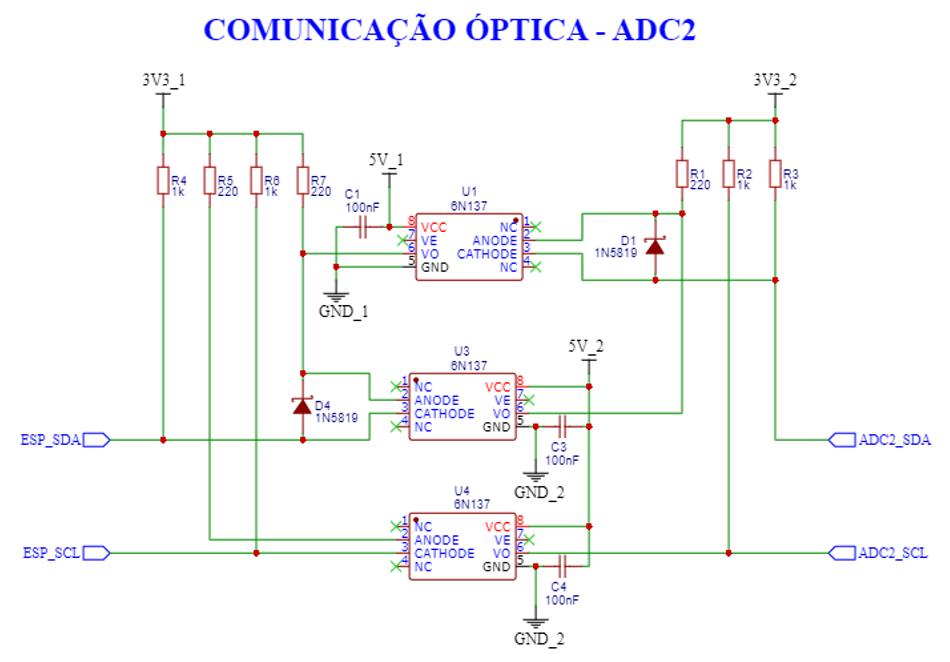
\includegraphics[width=1.0\textwidth]{figuras/circ-comunic.png}
    \fonte{}
\end{figure}

O circuito transforma pulsos \gls{$I^2$C} em sinais de luz e transfere estas informações para o outro circuito isolado, desacoplando estes. Para o correto funcionamento do circuito, devido a limitações técnicas dos \textit{optocouplers} escolhidos, é necessária a inserção de uma linha de 5 V para a alimentação do \gls{CI}, bem como o uso de uma linha de 3,3 V para a ativação dos LEDs internos deste chip, bem como o potencial de \textit{pull-up} para as linhas de comunicação \gls{$I^2$C}.

Como objetivo do trabalho, também é colocado como principal a modularidade do circuito, para se obter leituras de duas ou três fases diferentes. Inicialmente, foi considerado o uso do protocolo \gls{$I^2$C} também para a comunicação entre estes módulos. Porém, esta idéia foi descartada devido à complexidade de criação de um protocolo, ou dicionário, para estabelecer um modo comum de interação.

Também, para o demérito da utilização de tal topologia, são necessários muitos fios de interligação entre os módulos, sendo estes:

\begin{itemize}
    \item 5 V;
    \item 3,3 V;
    \item SDA;
    \item SCL e
    \item \textit{ground}.
\end{itemize}

Por estes dois grandes motivos e também por existirem alternativas mais simples, chegou-se a conclusão de que a utilização do protocolo \textit{ESP-NOW}, desenvolvido pela própria Espressif, para facilitar a comunicação entre chips desta que possuem \textit{WiFi}. Desta maneira, serão necessários somente 2 fios entre módulos, para o envio de um sinal de sincronização. Todo o restante da comunicação inicial é feito através deste protocolo.

Para a alimentação dos circuitos integrantes do protótipo, existem duas opções: baterias ou fontes. Como este será utilizado em bancada, foi escolhida a alimentação por fontes, pois estas não precisam ser trocadas frequentemente e é possível ligá-las à rede, além de algumas outras vantagens.

Neste projeto são utilizadas duas fontes isoladas galvanicamente, uma para alimentar o circuito de leitura de tensão e outra para alimentar o circuito de leitura de corrente, reduzindo ainda mais possíveis ruídos e interferências entre circuitos, mas também aumentando a confiabilidade do protótipo, pois como o objetivo é realizar leituras simultâneas de corrente e tensão, o isolamento entre eles é necessário para prevenir curtos.

Porém, o output das fontes escolhidas é de 12 V, não atendendo as necessidades de alimentação dos \gls{CI}s envolvidos e também do microcontrolador. Para isso, circuitos de regulação de tensão foram implementados, gerando duas saídas, como explícito na \autoref{fig:circ-conv-T}. Estes circuitos são iguais tanto para a leitura de tensão e de corrente, visto que estes tem as mesmas necessidades.

\begin{figure}[htb!]
    \caption{Circuito de regulação de tensão}
    \label{fig:circ-conv-T}
    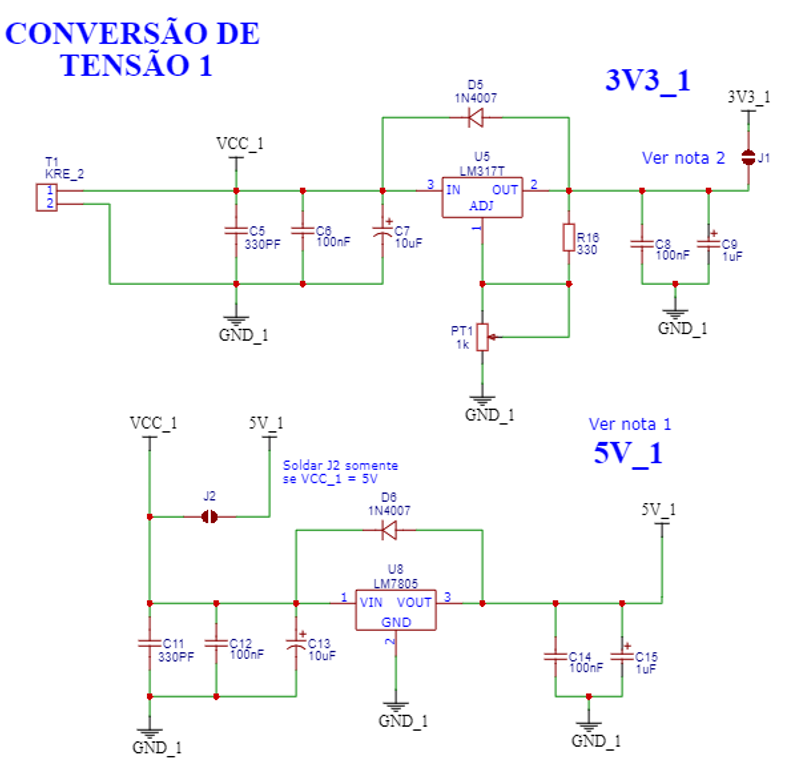
\includegraphics[width=0.8\textwidth]{figuras/circ-conv-T.png}
    \fonte{}
\end{figure}

A alimentação do ESP32 e também do circuito de comunicação isolada foi convencionada por especificação de projeto, para se manter um padrão e também suprir as necessidades de cada.

Por fim, um resumo de todas as partes constituintes e as decisões tomadas.

\begin{itemize}
    \item \textbf{Proteção de Entrada:} Foi decidida a utilização de uma proteção de entrada simplificada, baseada em modelos comerciais, pois não foi possível encontrar bibliografias relevantes e também não se possui equipamento especializado para fazer testes de proteção com segurança, visto que estes podem ser perigosos. Composta por fusíveis e um clamp para a corrente, varistores e um PTC para a tensão (junto com uma proteção TVS interna ao ADC escolhido), esta proteção básica coloca o protótipo dentro da classificação CAT III;
    \item \textbf{Condicionamento e Aquisição de Sinais:} Para a tensão, limita-se o valor máximo do sinal a ser obtido e este é encaminhado diretamente à entrada do ADC para leitura. Para a corrente, utiliza-se um resistor shunt para a obtenção do sinal. Os dois sinais serão lidos diferencialmente pelo ADC.
    \item \textbf{ADC:} O ADC escolhido foi o ADS1015, do tipo delta-sigma. Este foi escolhido por, além de suas capabilidades, suporte para comunicação em $I^2C$ e uma boa documentação sobre seu firmware.
    \item \textbf{Microcontrolador:} O MCU escolhido foi o ESP32, por ser um microcontrolador extremamente potente e possuir suporte para comunicações \textit{wireless} e por $I^2C$. Além disso, sua documentação técnica e o suporte tanto da Espressif quanto da comunidade que utiliza tal microcontrolador são de grande valor.
    \item \textbf{Alimentação:} O tipo de alimentação escolhido e implementado foi por fontes isoladas com reguladores internos para alimentar o circuito. Este método garante a maior segurança quanto à isolação das partes e também torna o protótipo independente de pilhas.
\end{itemize}

\subsection{Software e Firmware}\label{softfirm}

A programação do dispositivo é separada em duas etapas: \textit{Firmware} e \textit{Software}. O \textit{Firmware} é responsável por garantir a funcionalidade da comunicação do microcontrolador com os módulos \gls{ADC}, bem como manter a comunicação sem fio e sincronizar a amostragem do sinal.
Já o \textit{Software}, é responsável por receber as entradas do usuário e mostrar, efetivamente, através de gráficos e valores numéricos, as leituras de tensão, corrente, frequência, potências, etc.
Outra parte importante da programação trata-se da modularidade. Essa está presente tanto no \textit{Firmware} quanto no \textit{Software}. Trata-se da possibilidade de utilizar mais de um dispositivo em conjunto com um principal, permitindo a leitura de mais fases de maneira isolada.

\subsubsection{Disponibilidade do Circuito}\label{availability}

O circuito pode ser encontrado na integra no [ANEXO X] ao final do trabalho, bem como de maneira virtual no mesmo anexo. Dada a característica colaborativa da plataforma em que foi desenvolvido, permite que qualquer usuário clone esse circuito e o modifique gratuitamente.

\subsubsection{Firmware}\label{firmw}

O \textit{Firmware} é a parte crítica que roda diretamente no microcontrolador ESP32 e é responsável pela interface com os sensores, controle de comunicação sem fio e envio dos dados coletados para o \textit{Software} via WebSockets. Ele também gerencia a sincronização das leituras do ADC, garantindo que os dados de tensão e corrente sejam capturados e processados de forma precisa.

O desenvolvimento do \textit{Firmware} foi baseado em bibliotecas otimizadas para o ESP32, como a \textit{ESPAsyncWebServer} e a \textit{WebSocketsServer}, que permitem uma comunicação eficiente com o dispositivo remoto (celular ou computador). Além disso, foi utilizada a biblioteca \textit{ADS1015\_WE} para interface com o ADC externo ADS1015, permitindo leituras de alta precisão de sinais analógicos.

A sincronização entre os sinais de tensão e corrente é feita por meio de interrupções, que detectam o momento em que os dados estão prontos para leitura. Isso garante que as amostragens estejam alinhadas e que os gráficos e cálculos de potência sejam precisos. Para garantir a modularidade do sistema, o \textit{Firmware} também possui a capacidade de alterar a faixa de leitura da tensão e da corrente dinamicamente, de acordo com o comando enviado pelo usuário via WebSockets.

Uma parte importante do \textit{Firmware} é a implementação da máquina de estados \autoref{fig:maq-estado-simp}, que gerencia a comunicação com o dispositivo auxiliar. A implementação foi feita para ser expansível, permitindo a futura integração de múltiplos dispositivos sem a necessidade de grandes modificações no código.

\begin{figure}[htb!]
    \caption{Máquina de estados simplificada para apenas um dispositivo}
    \label{fig:maq-estado-simp}
    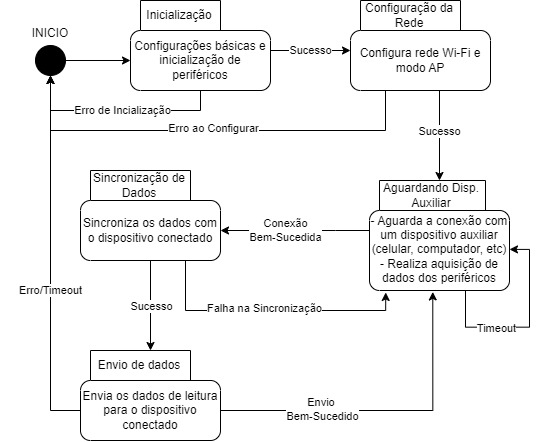
\includegraphics[width=1.0\textwidth]{figuras/Maquina-Estados-Simplificada.jpg}
    \fonte{}
\end{figure}

O processo de comunicação sem fio utiliza o protocolo \textit{WiFi} integrado do ESP32 para criar um ponto de acesso, facilitando a interação com o dispositivo móvel. O firmware também é responsável por lidar com a detecção de conexões e desconexões dos clientes WebSocket, ajustando o comportamento do sistema conforme necessário.

Seguindo a lógica proposta, o microcontrolador, ao ser energizado, completa sua rotina de \textit{setup} e permanece disponível para conexões. Após o estabelecimento da conexão, configura-se a relação principal entre o servidor, como \textit{master}, e o dispositivo conectado, como \textit{main client}. Ao acessar o IP do ESP32, ele serve à \textit{webpage} o HTML e JavaScript necessários para sua apresentação e interação.

Quando a leitura é iniciada, o microcontrolador executa todas as etapas necessárias, incluindo o envio do pulso de \textit{sync} (sincronização), a criação de um delta de tempo para estabelecer um ponto de referência zero, o que possibilita a sincronização das ondas, além do cálculo da frequência e do fator de potência. A aquisição dos dados em si também envolve uma série de processos específicos.

O \gls{ADC}, acompanhado pelo circuito de condicionamento de sinais, opera em dois modos de leitura: \textit{Data-Ready} e \textit{Single-Shot}.

No modo \textit{Single-Shot}, o processador solicita as leituras ao \gls{ADC}, que processa e envia os dados requisitados. Embora esse modo seja simples de implementar e bastante confiável, as limitações do chip escolhido tornam essa solução lenta para a aplicação em questão, alcançando uma taxa máxima de leitura de cerca de 500 \gls{SPS}, insuficiente para a aquisição desejada da forma de onda.

Optou-se, então, pelo modo \textit{Data-Ready}, que é mais complexo de implementar. Nesse modo, após cada leitura, o \gls{ADC} sinaliza ao microcontrolador levantando uma \textit{flag} (por exemplo, elevando um pino específico para 1) indicando que os dados estão prontos, aguardando a ação do processador. Quando o processador requisita os dados, eles são removidos do \textit{cache} do \gls{ADC}, reiniciando o ciclo de leitura. Com esse método, foi possível atingir uma taxa de 3300 \gls{SPS}, permitindo uma aquisição mais precisa da forma de onda.

Os valores adquiridos pelo \gls{ADC} são então processados pelo ESP32 para converterem-se em valores reais. Esse processamento começa com a seleção de uma faixa de leitura (\textit{range}) via o \textit{Programmable-gain Amplifier} (\gls{PGA}).

Uma vez processados, os dados puros são armazenados em uma \textit{struct}, conforme a estrutura da \autoref{tab:struct-graph}, serializados em formato JSON e enviados à \textit{webpage} para visualização. Caso não haja novas entradas do cliente, esse processo se repete indefinidamente.

\begin{table}[h!]
\centering
\caption{Chart data}
\begin{tabular}{|c|c|c|}
    \hline
    \textbf{Tipo} & \textbf{Nome da Variável} & \textbf{Descrição} \\ \hline
    int8\_t & chart\_id & Identificação do gráfico (usada somente para modularidade) \\ \hline
    int8\_t & voltage\_gain & Ganho de tensão a ser informado para o WebServer \\ \hline
    int8\_t & current\_type & Ganho/faixa de corrente a ser informada para o WebServer (mA, A, uA) \\ \hline
    int16\_t & voltage\_value[ ] & Array de valores das tensões lidas \\ \hline
    int16\_t & current\_value[ ] & Array de valores das correntes lidas \\ \hline
    int64\_t & voltage\_time[ ] & Array de valores dos tempos em que cada tensão foi lida \\ \hline
    int64\_t & current\_time[ ] & Array de valores dos tempos em que cada corrente foi lida \\ \hline
\end{tabular}
\label{tab:struct-graph}
\fonte{}
\end{table}

\subsubsection{Software}\label{softwa}

Toda a lógica de conversão dos valores de tensão e corrente em bits do \gls{ADC} para os valores reais é feita através de javascript em uma webpage. Dessa maneira, poupa-se informação transmitida pelo módulo, e utiliza-se um processamento mais robusto (do celular ou computador conectado) para os cálculos de potência.
Esta webpage, programada em HTML 5 para fazer a inserção de JavaScript e então utilizar Websocket, um protocolo de comunicação que fornece uma via de duas mãos para a conexão entre os servidores do microcontrolador, para cuidar da comunicação entre o ESP32 e o aparelho móvel, fará o tratamento dos dados e os apresentará para o usuário, em forma de gráficos e visualizadores numéricos representando a Tensão RMS, corrente RMS, frequência, Potências: aparente, reativa e ativa, e Fator de Potência.

\subsubsubsection{Tensão e Corrente}
Para diferentes configurações de escala de tensão, o código utiliza multiplicadores pré-definidos para converter os valores lidos para a tensão real. A \autoref{tab:softw-tensao} descreve os multiplicadores e a escala máxima correspondente:

\begin{table}[h!]
    \centering
    \caption{Tabela de multiplicadores de tensão}
    \begin{tabular}{|c|c|c|c|}
        \hline
        \textbf{Multiplicador} & \textbf{Tensão Máxima na Escala (V)} & \textbf{Ganho} & \textbf{Tensão Máxima (V)} \\
        \hline
        0.2 & 409.6 & 1 & 4.096 \\
        0.1 & 204.8 & 2 & 2.048 \\
        0.05 & 102.4 & 4 & 1.024 \\
        0.025 & 51.2 & 8 & 0.512 \\
        0.0125 & 25.6 & 16 & 0.256 \\
        \hline
    \end{tabular}
    \label{tab:softw-tensao}
    \fonte{}
\end{table}

Os valores foram obtidos analisando o circuito, de maneira a sempre manter a tensão na leitura abaixo dos 3.3V de tensão suportados pelo \gls{ADC}. Estes devem ser ajustados conforme a necessidade de calibração do dispositivo montado.

De maneira similar, o mesmo ocorre com a corrente. Porém, devido a aspectos construtivos do módulo, essa sempre está com o \gls{PGA} na escala \textit{x16}, alterando apenas os multiplicadores conforme a \autoref{tab:softw-corrente}.
Os ajustes para cada escala tratam-se dos valores de calibração que devem ser alterados conforme a necessidade após ter o dispositivo físico montado.

% Tabela de multiplicadores de corrente
\begin{table}[h!]
    \centering
    \caption{Tabela de multiplicadores de corrente}
    \begin{tabular}{|c|c|}
        \hline
        \textbf{Escala} & \textbf{Multiplicador} \\
        \hline
        A & $0.01875 \times \text{ajuste\_A}$ \\
        mA & $0.0001856 \times \text{ajuste\_mA}$ \\
        uA & $0.000001875 \times \text{ajuste\_uA}$ \\
        \hline
    \end{tabular}
    \label{tab:softw-corrente}
    \fonte{}
\end{table}

Os valores dos multiplicadores de corrente foram obtidos analisando o comportamento do circuito e fazendo as devidas conversões de tensão para corrente conforme o valor dos resistores utilizados em cada caso, veja \autoref{tab:softw-corrente-values}:

\begin{table}[h!]
    \centering
    \caption{Tabela de multiplicadores de corrente}
    \begin{tabularx}{\textwidth}{|X|X|X|X|X|X|X|}
        \hline
        \textbf{Range} & \textbf{Resistor shunt} & \textbf{Corrente (A)} & \textbf{Mult. do divisor resistivo} & \textbf{Tensão lida (V)} & \textbf{Mult. inicial (0,125mV/bit)} & \textbf{Mult. final (razão do resistor)} \\
        \hline
        uA & 100 & 0,001 & 1,5 & 0,1000 & 0,0001875 & 0,000001875 \\
        mA & 1,01 & 0,2 & 1,5 & 0,2020 & 0,0001875 & 0,000185644 \\
        A & 0,01 & 10 & 1,5 & 0,1000 & 0,0001875 & 0,018750 \\
        \hline
    \end{tabularx}
    \label{tab:softw-corrente-values}
    \fonte{}
\end{table}

\subsubsubsection{Apresentação Visual}

Os gráficos são gerados por uma biblioteca do JavaScript chamada Graph.js. Esta biblioteca possibilita a integração de vários gráficos, para a amostragem e apresentação tanto da tensão quanto da corrente simultaneamente, e também a utilização de um \textit{trigger} por programação, para ser possível a visualização da onda estabilizada. Este trigger funciona de forma a detectar a passagem da onda por um ponto escolhido e então sincronizar o gráfico de acordo, tornando aquele o ponto 0 visualizado e então estabilizando a onda.

A parte estrutural da página foi desenvolvida utilizando \gls{HTML}. Exemplos das telas durante a leitura podem ser vistos na \autoref{fig:webpage1} e \autoref{fig:webpage2}.

\begin{figure}[h!]
    \centering
    \caption{Detalhe do cabeçalho de informações da página da Web gerada pelo dispositivo}
    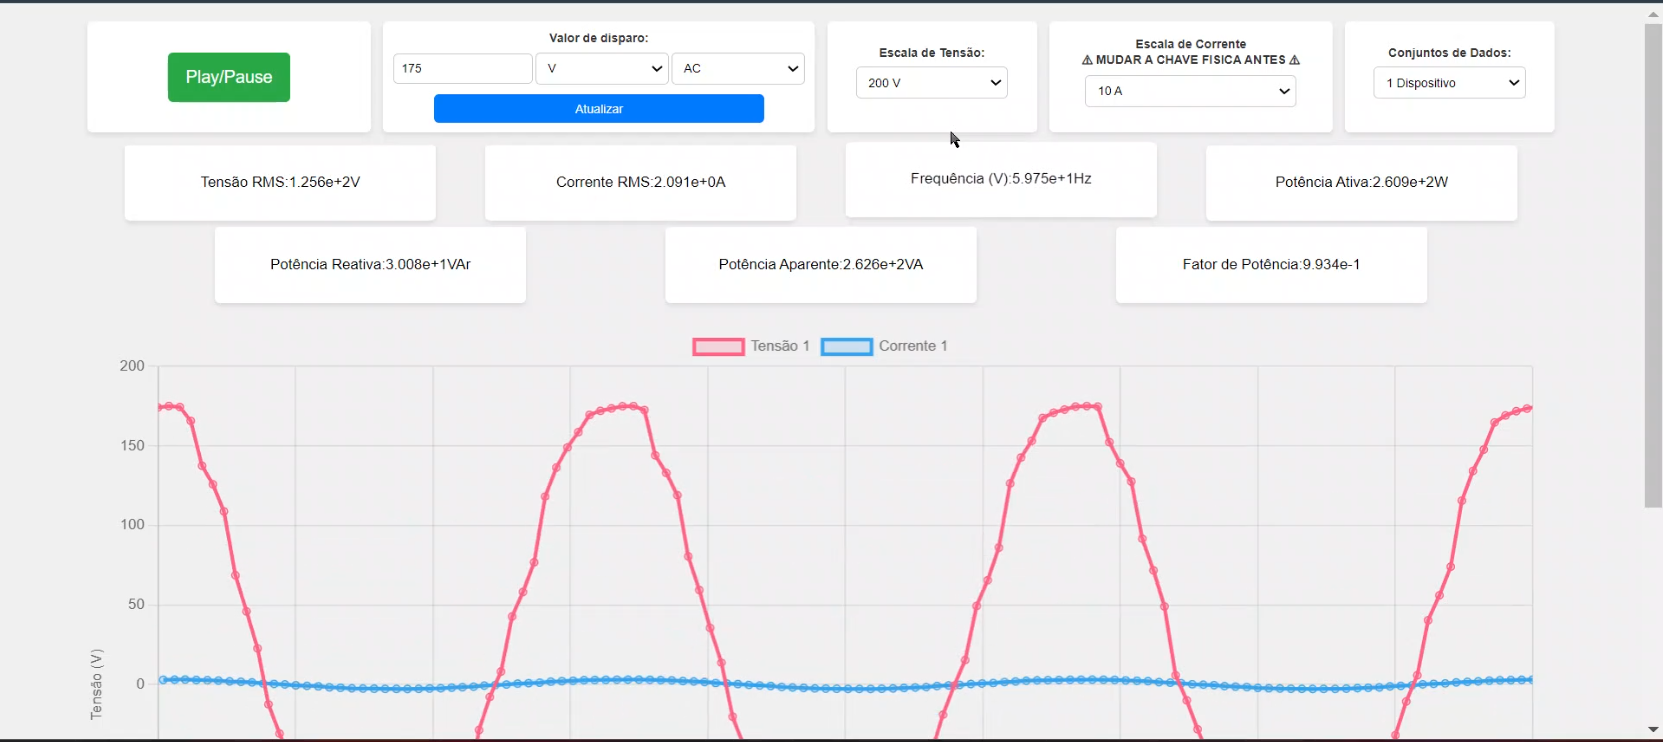
\includegraphics[width=\textwidth, height=\textheight, keepaspectratio]{webpage-tela1.png}
    \label{fig:webpage1}
    \fonte{}
\end{figure}

\begin{figure}[h!]
    \centering
    \caption{Detalhe do gráfico da página da Web gerada pelo dispositivo}
    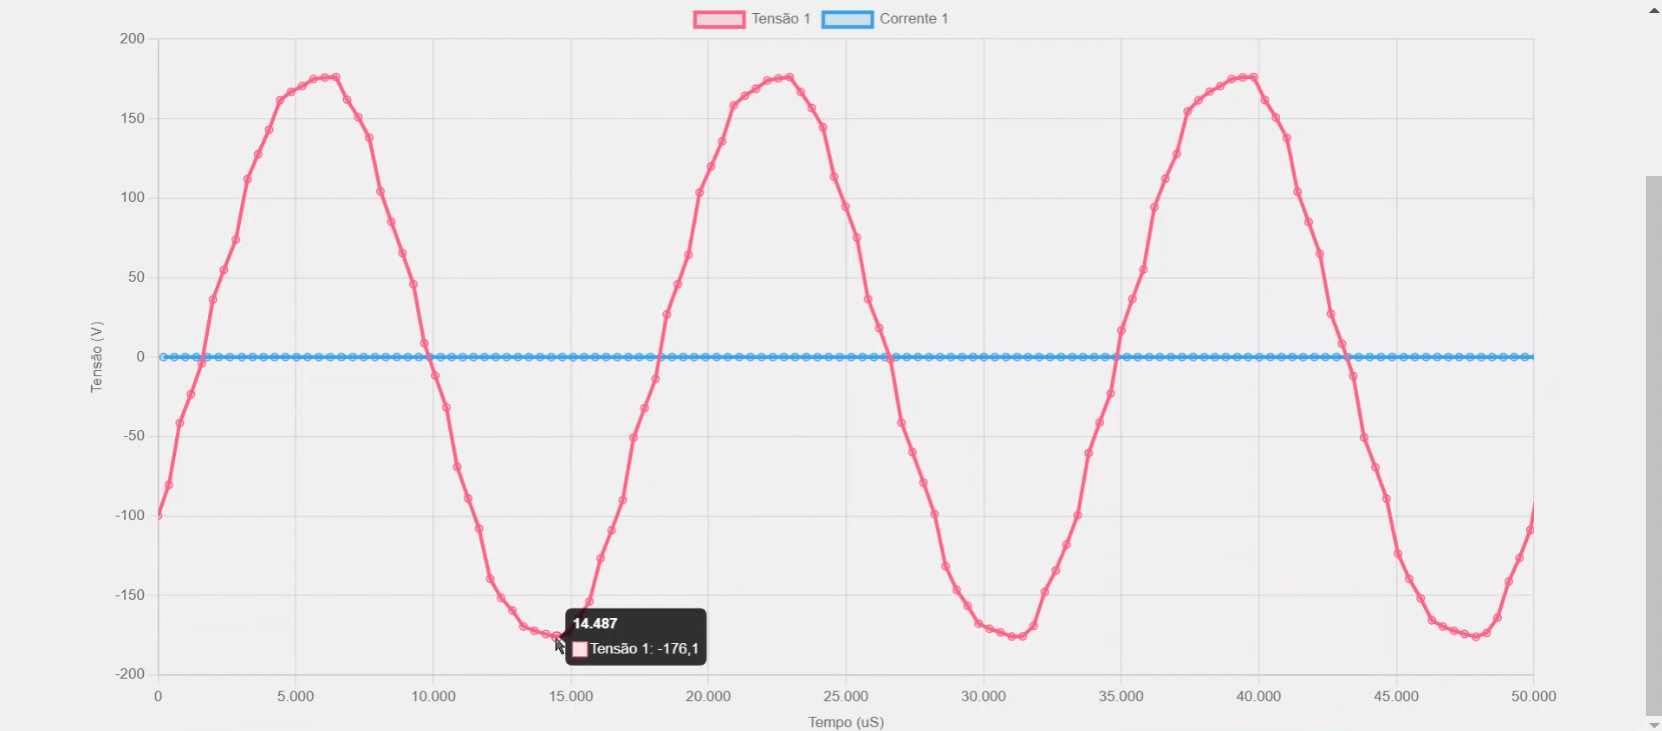
\includegraphics[width=\textwidth, height=\textheight, keepaspectratio]{webpage-tela2.png}
    \label{fig:webpage2}
    \fonte{}
\end{figure}

\subsubsection{Modularidade}\label{modular-softw}

Devido a dificuldades durante o desenvolvimento do projeto, não foi possível implementar por completo a função de modularidade entre os dispositivos. Dessa maneira, não é possível observar mais de um módulo ao mesmo tempo.
O conceito da comunicação, porém, foi testado utilizando-se dois módulos \textit{ESP32} e dados pré-programados de leitura, permitindo que fosse possível estabelecer o conceito da comunicação e elaborar a máquina de estados que define como a comunicação precisa ser tratada.

\begin{figure}[h!]
    \centering
    \caption{Máquina de Estados Completa}
    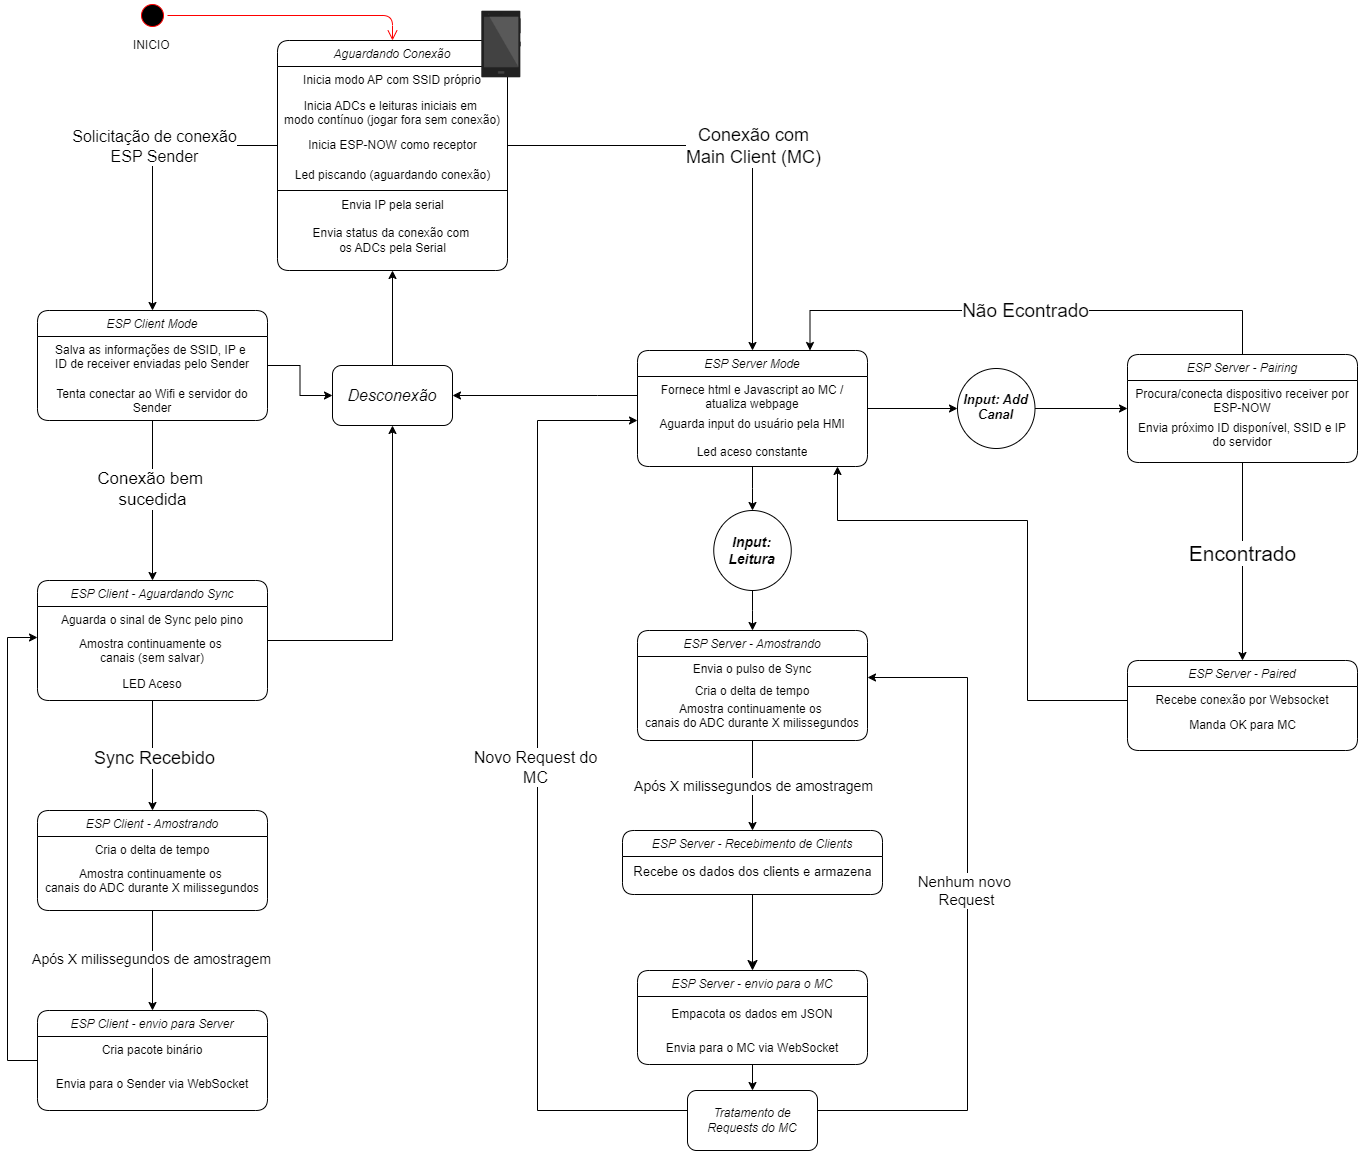
\includegraphics[width=\textwidth, height=\textheight, keepaspectratio]{state-machine-complete.png}
    \label{fig:maq-estados-completa}
    \fonte{}
\end{figure}

É possível observar pela \autoref{fig:maq-estados-completa} que sua implementação tornaria o código e o desenvolvimento desse trabalho extremamente complexos. Dessa forma, incentiva-se a continuação dessa proposta em trabalhos futuros.

Após o processo da máquina de estados padrão, apresentada na \autoref{fig:maq-estado-simp} - com a modularidade futuramente implementada - o funcionamento da máquina de estados completa se daria da seguinte forma:

Caso o cliente deseje adicionar um canal de leitura, o microcontrolador utiliza o protocolo \textit{ESP-NOW} para procurar e parear com um dispositivo adicional disponível.

Uma limitação do protocolo \textit{ESP-NOW} é o tamanho máximo de 255 bytes por pacote de dados. Um par de pontos de tensão e corrente ocupa cerca de 160 bits. Com essa limitação, é possível transmitir no máximo 12 pontos de uma forma de onda, o que é insuficiente, considerando que uma onda completa requer aproximadamente 55 pontos a uma taxa de 3300 \gls{SPS} e que, para uma análise adequada de uma rede trifásica, é necessário amostrar ao menos 3 ciclos de onda.

Assim, após o emparelhamento bem-sucedido, estabelece-se uma relação de \textit{client} com o dispositivo adicional, fornecendo-lhe todas as informações da rede necessárias para que ele acesse a mesma \textit{webpage} e \textit{Websocket}. Nesse momento, o uso do protocolo \textit{ESP-NOW} é finalizado, e toda a comunicação subsequente é realizada diretamente via \textit{Websocket}. Isso reduz a carga de processamento no microcontrolador e otimiza o tempo de comunicação e a transmissão de dados, pois o tamanho dos pacotes aumenta de 255 bytes para até 5 kilobytes.

Ao iniciar uma nova leitura via \textit{input} do cliente, um sinal de \textit{sync} é enviado do servidor \textit{master} para o módulo do canal adicional, estabelecendo assim uma referência temporal para sincronizar as leituras. A adição de canais é limitada a dois, permitindo a leitura trifásica.

\section{Materiais}\label{sec:materiais}

Esta seção está dedicada à lista de materiais utilizados para a confecção de um protótipo. Os preços indicados são validos somente para a data de confecção desta monografia, pois estão cotados de acordo com o que se foi pago para a confecção deste, sendo os componentes originados de várias lojas diferentes, online e físicas, na China e no Brasil e também em datas diferentes.

Nota-se também que para efeito de testes e de montagem do protótipo testado, não se foi considerada a proteção de entrada por dois fatores: primeiramente esta é extremamente cara e difícil de encontrar (em questão aos fusíveis). Outro motivo é a segurança dos autores, pois testes de proteção são perigosos necessitam aparatos especiais.

\begin{table}[h!]
\centering
\caption{Lista de Materiais e Custos}
\label{tab:Bookofmaterials}
\begin{tabular}{|l|c|c|c|}
\hline
\textbf{Material} & \textbf{Quantidade} & \textbf{Preço por Unidade (R\$)} & \textbf{Valor Total (R\$)} \\ \hline
ESP32 & 1 & 60,00 & 60,00 \\ \hline
ADC ADS1015 & 2 & 35,00 & 70,00 \\ \hline
Buzzer THT & 1 & 3,50 & 3,50 \\ \hline
Capacitor 100 nF & 15 & 0,25 & 3,75 \\ \hline
Capacitor 330 pF & 4 & 0,15 & 0,60 \\ \hline
Capacitor 10 µF & 4 & 0,20 & 0,80 \\ \hline
Capacitor 1 µF & 6 & 0,20 & 1,20 \\ \hline
Diodo Schottky 1N5819 & 4 & 0,25 & 1,00 \\ \hline
Diodo 1N4007 & 10 & 0,15 & 1,50 \\ \hline
Trimpot 1 K$\Omega$ & 4 & 3,60 & 14,40 \\ \hline
Transistor BC547 & 1 & 0,25 & 0,25 \\ \hline
Resistor 220 $\Omega$ & 6 & 0,10 & 0,60 \\ \hline
Resistor 1 k$\Omega$ & 13 & 0,10 & 1,30 \\ \hline
Resistor 330 $\Omega$ & 2 & 0,10 & 0,20 \\ \hline
Resistor 0 $\Omega$ & 4 & N/A & 0,00 \\ \hline
Resistor 3k3 $\Omega$ & 1 & 0,10 & 0,10 \\ \hline
Resistor 1\% 2 M$\Omega$ & 4 & 0,08 & 0,32 \\ \hline
Resistor 1\% 10 k$\Omega$ & 4 & 0,10 & 0,40 \\ \hline
Resistor 1\% 100 $\Omega$ & 4 & 0,20 & 0,80 \\ \hline
Resistor 1\% 1 $\Omega$ & 4 & 0,20 & 0,80 \\ \hline
Resistor SMD 1\% 10 m$\Omega$ & 1 & 0,30 & 0,30 \\ \hline
Varistor S05K385 & 2 & 3,00 & 6,00 \\ \hline
Fusível HRC 440 mA & 1 & 45,50 & 45,50 \\ \hline
Fusível HRC 11 A & 1 & 49,50 & 49,50 \\ \hline
Borne KRE2 & 3 & 1,30 & 3,90 \\ \hline
Borne KRE3 & 2 & 2,00 & 4,00 \\ \hline
Chave Alavanca 2 posições & 1 & 4,20 & 4,20 \\ \hline
LM317T & 2 & 2,30 & 4,60 \\ \hline
LM358 & 2 & 1,10 & 2,20 \\ \hline
LM7805 & 2 & 1,60 & 3,20 \\ \hline
6N137 & 6 & 3,20 & 19,20 \\ \hline
Barra de Pinos Fêmea 40x1 & 2 & 3,10 & 6,20 \\ \hline
Fonte Isolada & 2 & 12,50 & 25,00 \\ \hline
\textbf{TOTAL} &  &  & \textbf{335,32} \\ \hline
\end{tabular}
\fonte{}
\end{table}


\section{\textit{Casing}}\label{Casing}

Para a confecção do invólucro, ou \textit{casing} do protótipo, foi utilizado uma plataforma também gratuita de modelagem, chamada \textit{Onshape}.

Foram tiradas as medidas de um módulo de bancada de madeira, que suporta os equipamentos em bancadas dos laboratórios em questão, como demonstrado na \autoref{fig:Modulo-Base-Frente} e então feito o design com estas e também respeitando o tamanho e configuração da \gls{PCB}.

\begin{figure}[htb!]
    \caption{Módulo de Bancada}
    \label{fig:Modulo-Base-Frente}
    \includegraphics[width=0.8\textwidth]{figuras/Modulo-Base-Frente.jpg}
    \fonte{}
\end{figure}

O modelo foi pensado para ser o mais simples possível de ser impresso em 3D e modificado. Possui espaço para a placa e periféricos necessários.
Devido a dificuldades no desenvolvimento do trabalho, o encapsulamento não foi fabricado, apenas teve seu dimensional analisado em ambiente virtual.
Uma visão geral do modelo pode ser visto na \autoref{fig:osciloboy-isometrico}, juntamente de uma representação simplificada do suporte de madeira citado anteriormente.
O detalhe dos suportes internos pode ser visto na \autoref{fig:osciloboy-detalhes}.

\begin{figure}[htb!]
    \caption{Modelo virtual do encapsulamento}
    \label{fig:osciloboy-isometrico}
    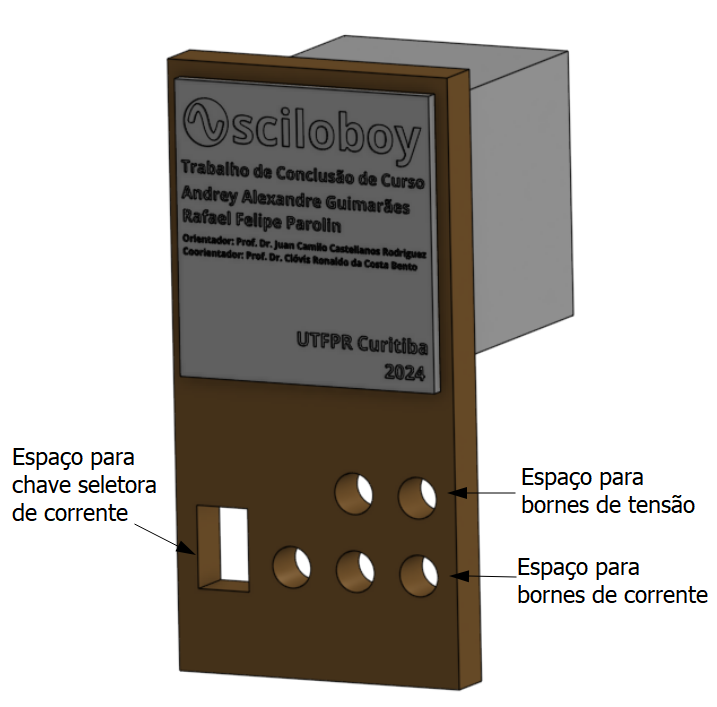
\includegraphics[width=0.8\textwidth]{figuras/osciloboy-case-1.png}
    \fonte{}
\end{figure}

\begin{figure}[htb!]
    \caption{Detalhes de suportes para PCB e periféricos}
    \label{fig:osciloboy-detalhes}
    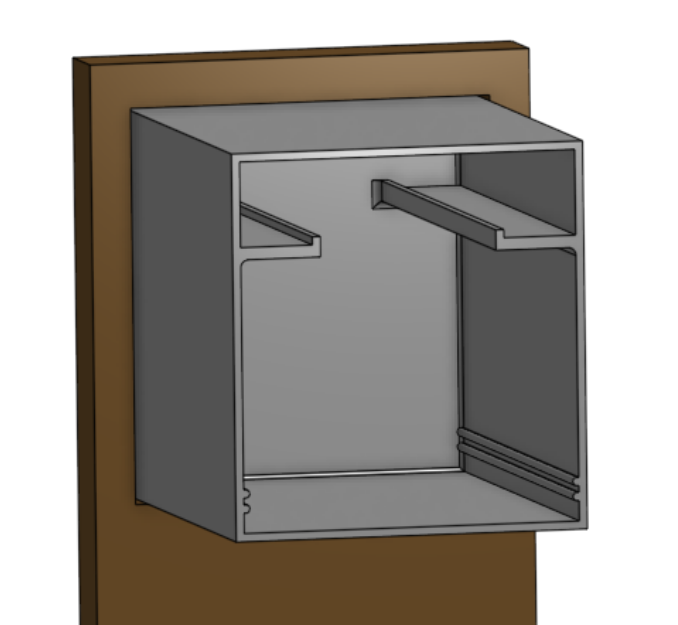
\includegraphics[width=0.8\textwidth]{figuras/osciloboy-case-2.png}
    \fonte{}
\end{figure}

Assim como os demais elementos desse projeto, pode ser encontrado no [ANEXO X] ao final do trabalho, bem como, dado a característica colaborativa da plataforma, pode ser clonado e modificado sem nenhum custo, conforme a necessidade do usuário.

%% Comente para remover este item

%% Capítulo
%%%% CAPÍTULO 4 - RESULTADOS E DISCUSSÃO

\chapter{Resultados}\label{cap:resultados}%% Comente para remover este item

%% Capítulo - esse capítulo contém exemplos para melhor uso do modelo Latex
%% Na versão final do TCC esse capítulo deve ser removido utilizando o sinal %
%%%%% CAPÍTULO - EXEMPLO
%%
%% Capítulo de informações e exemplos de utilização deste modelo.

%% Título e rótulo de capítulo (rótulos não devem conter caracteres especiais, acentuados ou cedilha)
\chapter{Informações e Exemplos de Utilização deste Modelo}\label{cap:exemplo}

Devido à necessidade de padronização em trabalhos acadêmicos (teses, dissertações, trabalhos de conclusão de curso, etc.), são utilizadas neste documento algumas regras básicas para estruturação e formatação.

O presente documento/\textit{template} foi produzido em parceria entre a \gls{utfpr} de Pato Branco e a \gls{utfpr} de Campo Mourão. Assim, derivado do \gls{utfprpbtex}\index{UTFPRPBTeX@\utfprpbtex} e de alterações implementadas pela UTFPR de Campo Mourão, surge o \utfprtex, como um proposta de um modelo \latex que pode ser utilizado por qualquer campus da \gls{utfpr} para elaboração de trabalhos acadêmicos segundo as normas definidas pela \gls{abnt}\index{ABNT}. Este modelo foi desenvolvido em linguagem de editoração \gls{tex}\index{TeX@\TeX}/\gls{latex}\index{LaTeX@\latex} com base no modelo \gls{abntex2}\index{abnTeX2@\abnTeX} \cite{abnTeX2:2013}, que atende os requisitos das normas da ABNT para elaboração de documentos técnicos e científicos brasileiros.

Os principais arquivos do modelo são: 
\begin{itemize}
    \item \texttt{main.tex} - é o arquivo principal que relaciona todos os outros arquivos, neste você pode remover ou adicionar elementos textuais (capítulos, etc);
    \item \texttt{configuracoes.tex} - contém os pacotes a serem utilizados pelo ambiente, bem como a criação de comandos do \latex;
    \item \texttt{variaveis.tex} - contém variáveis, como nome do autor, orientador, título, banca e que devem ser alterados para atender cada trabalho;
    \item \texttt{main.bib} - contém as referências bibliográficas;
    \item \texttt{readme.md} - são informações a respeito do template \latex;
    \item \texttt{utfpr.cls} - mantém a formatação do texto - \textbf{não altere esse arquivo a menos que você saiba o que está fazendo}.
\end{itemize}

Além dos arquivos, o \textit{template} contém diretórios/pastas, para ajudar a organizar o trabalho, sendo essas:
\begin{itemize}%% Lista de itens
\item \texttt{PreTexto} - contém arquivos, com nomes auto descritivos, que representam elementos pré textuais como:  resumo, abstract, agradecimentos, siglas, epigrafe, etc;
\item \texttt{capitulos} -  contém arquivos, com nomes auto descritivos, que representam os capítulos do texto, como por exemplo: introdução, metodologia, conclusão, etc. Para adicionar ou remover um capítulo é necessário alterar o arquivo \texttt{main.tex} - ver exemplos no próprio arquivo;
\item \texttt{figuras}  - contém as figuras/imagens utilizadas no texto;
\item \texttt{PosTexto} - contém elementos pós textuais como: anexo, apêndice, etc.
\end{itemize}

A codificação de caracteres em todos os arquivos é \texttt{UTF8}, tanto no modelo \gls{abntex2}\index{abnTeX2@\abnTeX} quanto no modelo \gls{utfprpbtex}\index{UTFPRPBTeX@\utfprtex}. Portanto, é necessário que seja utilizada a mesma codificação nos documentos a serem desenvolvidos, inclusive nos arquivos de base bibliográfica. Diversos editores de arquivos fonte do \gls{latex}\index{LaTeX@\latex} são capazes de manipular e/ou converter entre diferentes codificações, por exemplo, o ``Texmaker\index{Texmaker}'' (disponível em \url{http://www.xm1math.net/texmaker/}). 
%Recomenda-se, sempre que for manipular e/ou substituir um dos arquivos constituintes deste modelo, manter uma cópia do original num local seguro e/ou renomear esta cópia do original para que possa ser utilizada como um exemplo no desenvolvimento do seu próprio arquivo. Por exemplo, quando for criar o seu ``Capítulo 1'', fazer uma cópia do arquivo original \texttt{capitulo1.tex}, renomeando-o para \texttt{capitulo1.original.tex}, por exemplo, e realizar as alterações e/ou modificações no arquivo \texttt{capitulo1.tex}.

Este capítulo\label{errata:capitulo} de exemplo tem por finalidade a definição e a apresentação de alguns comandos do \gls{latex}\index{LaTeX@\latex} e/ou dos modelos \gls{abntex2}\index{abnTeX2@\abnTeX} e \gls{utfprpbtex}\index{UTFPRPBTeX@\utfprtex}. O presente documento não se constitui um manual, tampouco uma apostila de \gls{latex}\index{LaTeX@\latex}, visto que existe uma grande quantidade de material de referência disponível na Internet, como por exemplo em \url{http://en.wikibooks.org/wiki/LaTeX}.

Os capítulos devem conter uma introdução e um fecho. A introdução fornece ao leitor uma breve descrição do que será tratado no capítulo, enquanto o fecho apresenta comentários finais sobre o que foi desenvolvido no capítulo. Os capítulos podem ser divididos em seções\label{errata:secao}. Esta divisão deve ser lógica (temática) e não física (por tamanho). O número ideal de seções é impossível de se precisar. Entretanto, um capítulo com uma única seção, possivelmente, deverá ser agregado ao capítulo anterior ou posterior. Um capítulo com quinze seções, possivelmente, deverá ser subdividido em dois capítulos. Capítulos, seções e subseções\label{errata:subsecao} devem ser rotulados para que possam ser referenciados em qualquer parte do texto. Exemplo: O \autoref{cap:exemplo} é gerado, rotulado e referenciado pelos comandos \verb|\chapter{Informações e...}|, \verb|\label{cap:exemplo}| e \verb|\autoref{cap:exemplo}|, respectivamente.

%% Título e rótulo de seção (rótulos não devem conter caracteres especiais, acentuados ou cedilha)
\section{Título da seção secundária}\label{sec:secsec}

Seções secundárias são divisões do conteúdo das seções primárias. A \autoref{sec:secsec} é gerada, rotulada e referenciada pelos comandos \verb|\section{Título da Seção Secundária}|, \verb|\label{sec:secsec}| e \verb|\autoref{sec:secsec}|, respectivamente.

%% Título e rótulo de seção (rótulos não devem conter caracteres especiais, acentuados ou cedilha)
\subsection{Título da seção terciária}\label{ssec:secterc}

Seções terciárias são divisões do conteúdo de seções secundárias. A \autoref{ssec:secterc} é gerada, rotulada e referenciada pelos comandos \verb|\subsection{Título da Seção Terciária}|, \verb|\label{ssec:secterc}| e \verb|\autoref{ssec:secterc}|, respectivamente.

%% Título e rótulo de seção (rótulos não devem conter caracteres especiais, acentuados ou cedilha)
\subsubsection{Título da seção quartenária}\label{sssec:secquart}

Seções quartenárias são divisões do conteúdo de seções terciárias. A \autoref{sssec:secquart} é gerada, rotulada e referenciada pelos comandos \verb|\subsubsection{Título da seção quartenária}|, \verb|\label{sssec:secquart}| e \verb|\autoref{sssec:secquart}|, respectivamente.

%% Título e rótulo de seção (rótulos não devem conter caracteres especiais, acentuados ou cedilha)
\section{Exemplo de título de seção secundária com um texto muito longo que pode ocupar mais de uma linha}\label{sec:sectitulolongo}

A \autoref{sec:sectitulolongo} é um exemplo de título de seção secundária com texto muito longo, formatado automaticamente de acordo com \citeonline[subseções 5.2.2 a 5.2.4]{NBR14724:2011} e \citeonline[subseções 3.1 a 3.8]{NBR6024:2012}. Segundo as normas, o título de seção deve estar alinhado à esquerda e a segunda e demais linhas devem iniciar logo abaixo da primeira palavra da primeira linha.

%% Título e rótulo de seção (rótulos não devem conter caracteres especiais, acentuados ou cedilha)
\section{Elementos pré-textuais}\label{sec:elempretext}

Alguns elementos pré-textuais do presente documento são gerados automaticamente pelo \gls{utfprpbtex}\index{UTFPRPBTeX@\utfprtex}. Para adicionar e/ou alterar as informações apresentadas na capa, na folha de rosto %, na ficha catalográfica 
e na folha de aprovação deve-se editar o arquivo \texttt{variaveis.tex}. %Os dados informados neste arquivo também são utilizados para gerar a referência do trabalho na errata, no resumo e no \textit{abstract}.

Para adicionar e/ou alterar o texto da errata, da dedicatória, dos agradecimentos, da epígrafe, do resumo e do \textit{abstract} deve-se editar seus respectivos arquivos presentes no diretório ``PreTexto'': \texttt{errata.tex}, \texttt{dedicatoria.tex}, \texttt{agradecimentos.tex}, \texttt{epigrafe.tex}, \texttt{resumo.tex} e \texttt{abstract.tex}.

As listas de algoritmos, de ilustrações e de tabelas são geradas automaticamente pelo \gls{utfprpbtex}\index{UTFPRPBTeX@\utfprtex}. Os itens destas listas são gerados a medida que forem sendo inseridos no texto do documento. 

A lista de abreviaturas, siglas e acrônimos pode ser gerada automaticamente por meio do arquivo \texttt{entradas-acronimos.tex}, utilizando o pacote \texttt{glossaries}\footnote{Detalhes sobre comandos para geração de abreviaturas, siglas e acrônimos utilizando o pacote \texttt{glossaries} são apresentadas na \autoref{sec:acronimos}.}, ou por meio da edição do arquivo \texttt{lista-acronimos.tex}. A lista de símbolos pode ser gerada automaticamente utilizando o pacote \texttt{nomencl}\footnote{Detalhes sobre comandos para geração de símbolos utilizando o pacote \texttt{nomencl} são apresentadas na \autoref{sec:simbolos}.} ou mediante a edição do arquivo \texttt{lista-simbolos.tex}. Os arquivos citados estão no diretório ``PreTexto''. O sumário é o último elemento pré-textual e também é gerado automaticamente pelo \gls{utfprpbtex}\index{UTFPRPBTeX@\utfprtex}.

%% Título e rótulo de seção (rótulos não devem conter caracteres especiais, acentuados ou cedilha)
\section{Regras gerais de apresentação}\label{sec:regrasgerais}

As regras gerais de apresentação, definidas na sequência, já estão predefinidas no modelo \gls{utfprpbtex}\index{UTFPRPBTeX@\utfprtex}. Algumas destas regras podem ser alteradas, por comandos apropriados do \gls{latex}\index{LaTeX@\latex}, do \gls{abntex2}\index{abnTeX2@\abnTeX} ou do \gls{utfprpbtex}\index{UTFPRPBTeX@\utfprtex}, no preâmbulo do arquivo principal \texttt{configuracoes.tex} ou em outras partes do documento, por exemplo, nos capítulos.

\begin{itemize}%% Lista de itens
\item Configuração das margens: deve-se usar margens superior e esquerda de \SI{3}{cm}; e margens inferior e direita de \SI{2}{cm}; em papel formato A4 ($\SI{21}{cm} \times \SI{29,7}{cm}$);
\item Recomenda-se o uso de fonte tipo Arial ou Times New Roman, tamanho 12 para o texto e tamanho 10 para citações de mais de três linhas, notas de rodapé e legendas dos algoritmos, ilustrações e tabelas;
\item O parágrafo deve aparecer com recuo na primeira linha de \SI{1,5}{cm}, justificado, sem espaçamento anterior ou posterior;
%\item Os elementos como: o resumo, as notas, as referências, as legendas das ilustrações e tabelas, a natureza do trabalho, o objetivo, o nome da instituição a que é submetida e a área de concentração devem ser digitados em espaço simples.
\item A numeração progressiva para as seções do texto deve ser adotada para evidenciar a sistematização do conteúdo do trabalho;
\item Para os títulos das seções não se utilizam pontos, hífen, travessão, ou qualquer sinal após o indicativo de seção ou de título;
\item Para as seções primárias: utiliza-se negrito e caixa alta;
\item Para as seções secundárias: título em negrito, iniciado em letra maiúscula e demais letras minúsculas;
\item Para as seções terciárias: somente a primeira letra do título da seção em
maiúscula;
\item Para as seções quaternárias: título da seção sublinhado, com inicial em letra maiúscula e demais letras minúsculas.
\item No sumário, os títulos das seções devem aparecer exatamente iguais ao que estão contidos no trabalho.
\end{itemize}

\caixa{Atenção}{No \latex é necessário manter os títulos apenas com a primeira letra maiúscula e o restante em minúsculo, o retante é controlado pelo \latex, então não é necessário se preocupar com a formatação!}

Recomenda-se evitar, sempre que possível, o uso dos seguintes recursos (ou enfeites) no documento:

\begin{itemize}%% Lista de itens
\item \textbf{o uso de negrito;}
\item \textit{o uso de itálico (exceto em palavras em outra língua);}
\item \texttt{texto em diferente fonte como máquina de escrever;}
\item \underline{o uso de texto sublinhado;}
\item o uso excessivo de\footnote{Notas de rodapé.}.
\end{itemize}

\noindent Lembre-se: um texto ``limpo'' é mais agradável de ler que um texto ``enfeitado''.

%% Título e rótulo de seção (rótulos não devem conter caracteres especiais, acentuados ou cedilha)
\subsection{Espaçamento}\label{sec:espacamento}

\begin{itemize}%% Lista de itens
%\item O resumo, o \textit{abstract}, as notas, as referências, as legendas das ilustrações e tabelas e a natureza do trabalho devem ser digitadas em espaço simples.
\item Todo o texto deve ser formatado com espaço entre linhas de um fator de 1,5 (sem espaçamento antes/depois).
\item As citações com mais de três linhas devem ser em espaço simples e com recuo de \SI{4}{cm} da margem esquerda.
\item As referências, ao final do trabalho, devem ser separadas entre si por um espaços simples, e na mesma referência o espaço é simples.
%\item Os títulos das seções secundárias devem ser separados do texto que os precede por dois espaços entre linhas de um fator de 1,5.
\item As seções primárias devem iniciar em páginas distintas.
\end{itemize}

O recuo na primeira linha, espaço entre a margem e o início do parágrafo, pode ser redefinido definido pelo comando:

\begin{SingleSpacing}%% Ambiente SingleSpacing
\begin{verbatim}
\setlength{\parindent}{1.5cm}
\end{verbatim}
\end{SingleSpacing}

O espaçamento entre um parágrafo e outro\index{espaçamento!entre os parágrafos} pode ser redefinido pelo comando:

\begin{SingleSpacing}%% Ambiente SingleSpacing
\begin{verbatim}
\setlength{\parskip}{0mm} %% Tente também \onelineskip
\end{verbatim}
\end{SingleSpacing}

O controle do espaçamento entre linhas\index{espaçamento!entre as linhas} pode ser redefinido pelo comando:

\begin{SingleSpacing}%% Ambiente SingleSpacing
\begin{verbatim}
\OnehalfSpacing %% Espaçamento um e meio (padrão)
\DoubleSpacing  %% Espaçamento duplo
\SingleSpacing  %% Espaçamento simples
\end{verbatim}
\end{SingleSpacing}

Para isso, também estão disponíveis os ambientes:

\begin{SingleSpacing}%% Ambiente SingleSpacing
\begin{verbatim}
\begin{SingleSpacing} ...     \end{SingleSpacing}
\begin{Spacing}{<factor>} ... \end{Spacing}
\begin{OnehalfSpacing} ...    \end{OnehalfSpacing}
\begin{OnehalfSpacing*} ...   \end{OnehalfSpacing*}
\begin{DoubleSpacing} ...     \end{DoubleSpacing}
\begin{DoubleSpacing*} ...    \end{DoubleSpacing*}
\end{verbatim}
\end{SingleSpacing}

Para mais informações, consulte \citeonline[p. 47-52 e 135]{Wilson2010}.

\subsection{Exemplo de quantidades de subseções}\label{sec:exSubsec}

Quando um item é dividido, precisa ter pelo menos dois sub-itens (não pode ter apenas um), por exemplo para ter a subseção 4.1 é obrigatório ter pelo menos a subseção 4.2, não pode somente a primeira subseção.

%% Título e rótulo de seção (rótulos não devem conter caracteres especiais, acentuados ou cedilha)
\section{Enumerações: alíneas e subalíneas}\label{sec:enumeracoes}\index{alíneas}\index{subalíneas}

Quando for necessário enumerar os diversos assuntos de uma seção que não possua título, esta deve ser subdividida em alíneas\index{alíneas} \cite[subseção 4.2]{NBR6024:2012}:

\begin{alineas}%% Ambiente alineas
\item os diversos assuntos que não possuam título próprio, dentro de uma mesma seção, devem ser subdivididos em alíneas\index{alíneas};
\item o texto que antecede as alíneas\index{alíneas} termina em dois pontos;
\item as alíneas\index{alíneas} devem ser indicadas alfabeticamente, em letra minúscula, seguida de parêntese. Utilizam-se letras dobradas, quando esgotadas as letras do alfabeto;
\item as letras indicativas das alíneas\index{alíneas} devem apresentar recuo em relação à margem esquerda;
\item o texto da alínea deve começar por letra minúscula e terminar em ponto-e-vírgula, exceto a última alínea que termina em ponto final;
\item o texto da alínea deve terminar em dois pontos, se houver subalínea;
\item a segunda e as seguintes linhas do texto da alínea começa sob a primeira letra do texto da própria alínea;
\item subalíneas\index{subalíneas} \cite[subseção 4.3]{NBR6024:2012} devem ser conforme as alíneas\index{alíneas} a seguir:
\begin{alineas}%% Ambiente alineas
\item as subalíneas\index{subalíneas} devem começar por travessão seguido de espaço;
\item as subalíneas\index{subalíneas} devem apresentar recuo em relação à alínea;
\item o texto da subalínea deve começar por letra minúscula e terminar em ponto-e-vírgula. A última subalínea deve terminar em ponto final, se não houver alínea subsequente;
\item a segunda e as seguintes linhas do texto da subalínea começam sob a primeira letra do texto da própria subalínea.
\end{alineas}
\item no \gls{abntex2}\index{abnTeX2@\abnTeX} estão disponíveis os ambientes \texttt{incisos} e \texttt{subalineas}, que em suma são o mesmo que se criar outro nível de \texttt{alineas}, como nos exemplos à seguir:
\begin{incisos}%% Ambiente incisos
\item \textit{um novo inciso em itálico}\index{incisos}.
\end{incisos}
\item Alínea em \textbf{negrito}:
\begin{subalineas}%% Ambiente subalineas
\item \textit{uma subalínea em itálico};
\item \underline{\textit{uma subalínea em itálico e sublinhado}}.
\end{subalineas}
\item última alínea com \emph{ênfase}.
\end{alineas}

%% Título e rótulo de seção (rótulos não devem conter caracteres especiais, acentuados ou cedilha)
\section{Citações}\label{sec:citacoes}

O \gls{utfprpbtex}\index{UTFPRPBTeX@\utfprtex} está configurado para produzir as citações no texto no estilo alfabético (autor-data), segundo as normas \gls{abnt}\index{ABNT}, por meio dos comandos do \gls{abntex2}\index{abnTeX2@\abnTeX} \cite{abnTeX2:2013Cite,abnTeX2:2013CiteAlf}. A lista dos principais comandos são apresentadas a seguir:

\begin{itemize}%% Lista de itens
\item \verb|\cite{rótulo}| -- para gerar citação implícita. Por exemplo, a citação ``\ldots\ \cite{Thompson2001}\ldots'' é gerada pelo comando \verb|\cite{Thompson2001}| ou pelo atalho \verb|\citep{Thompson2001}|, definido em \texttt{utfprpb.tex}.
\item \verb|\citeonline{rótulo}| -- para gerar citação explícita. Por exemplo a citação ``\ldots\ conforme proposto por \citeonline{Thompson2001}\ldots'' é gerada pelo comando \verb|\citeonline{Thompson2001}| ou pelo atalho \verb|\citet{Thompson2001}|, definido em \texttt{utfprpb.tex}.
\item \verb|(\citeauthor{rótulo})| -- para gerar citação implícita somente do autor. Por exemplo, a citação ``\ldots\ (\citeauthor{Thompson2001})\ldots'' é gerada pelo comando \verb|(\citeauthor{Thompson2001})| ou pelo atalho \verb|\citepa{Thompson2001}|, definido em \texttt{utfprpb.tex}.
\item \verb|\citeauthoronline{rótulo}| -- para gerar citação explícita somente do autor. Por exemplo, a citação ``\ldots\ conforme a relação de \citeauthoronline{Thompson2001}\ldots'' é gerada pelo comando \verb|\citeauthoronline{Thompson2001}| ou pelo atalho \verb|\citeta{Thompson2001}|, definido em \texttt{utfprpb.tex}.
\item \verb|(\citeyear{rótulo})| -- para gerar citação implícita somente do ano. Por exemplo, a citação ``\ldots\ (\citeyear{Thompson2001})\ldots'' é gerada pelo comando \verb|(\citeyear{Thompson2001})| ou pelo atalho \verb|\citepy{Thompson2001}|, definido em \texttt{utfprpb.tex}.
\item \verb|\citeyear{rótulo}| -- para gerar citação explícita somente do ano. Por exemplo, a citação ``\ldots\ no ano de \citeyear{Thompson2001}\ldots'' é gerada pelo comando \verb|\citeyear{Thompson2001}| ou pelo atalho \verb|\citety{Thompson2001}|, definido em \texttt{utfprpb.tex}.
\end{itemize}

Informações sobre a utilização dos comandos listados acima e os demais comandos para geração de referências, utilizados pelo \gls{abntex2}\index{abnTeX2@\abnTeX}, podem ser encontradas em \citeonline{abnTeX2:2013Cite,abnTeX2:2013CiteAlf}, disponíveis em \url{http://www.abntex.net.br/}.

\gls{latex}\index{LaTeX@\latex} utiliza um arquivo externo (em separado) para o banco de dados das referências citadas no texto. Este arquivo é compilado pelo \gls{bibtex}\index{BibTeX@Bib\TeX} e deve possuir a extensão \texttt{bib}, como nos arquivos \texttt{referencias.bib} e \texttt{referencias-modelos.bib} presentes no diretório ``PosTexto'', utilizados neste documento. O arquivo \texttt{referencias-modelos.bib} apresenta exemplos dos seguintes estilos de referência aceitos pelo \gls{bibtex}\index{BibTeX@Bib\TeX}:

\begin{itemize}%% Lista de itens
\item anais de simpósios \citep{Alt1995,Pirmez2002};
\item artigos em anais de simpósios \citep{Faina2001};
\item artigos em coletâneas de artigos \citep{Pinto2000};
\item artigos em revistas \citep{Guimaraes2003};
\item capítulos de livros \citep{Santos2000};
\item livretos \citep{Thompson2001};
\item livros \citep{Pedrycz1998};
\item manuais técnicos \citep{IONA1999};
\item miscelânea \citep{Cruz2003};
\item páginas na Internet \cite[acessado em 1 de janeiro de 2004]{Larsson2003} (utilizar a data do último acesso à página);
\item relatórios técnicos \citep{OMG2000};
\item teses de mestrado \citep{SantosFilho2003};
\item teses de doutorado \citep{Faina2000};
\item trabalhos não publicados \citep{Sichman2002}.
\end{itemize}

\subsection{Programas úteis para citações}\label{sec:progUteisCitacoes}

Existem alguns programas para gerenciamento de banco de dados de referências bibliográficas (arquivos \texttt{bib}) do \gls{bibtex}\index{BibTeX@Bib\TeX}. O ``JabRef'' é um exemplo destes programas e está disponível em: \url{http://jabref.sourceforge.net/}.

%% Título e rótulo de seção (rótulos não devem conter caracteres especiais, acentuados ou cedilha)
\subsection{Citações diretas}\label{sec:citacoesdiretas}\index{citações!diretas}

O ambiente \texttt{citacao} permite a inclusão de citações diretas que ocupam mais de três linhas:

\begin{citacao}%% Ambiente citacao
As citações diretas no texto, que ocupam mais de três linhas, devem ser destacadas com recuo de \SI{4}{cm} da margem esquerda, com letra menor que a do texto utilizado e sem as aspas. No caso de documentos datilografados, deve-se observar apenas o recuo \cite[subseção 5.3]{NBR10520:2002}.
\end{citacao}

\noindent Esta citação direta com mais de três linhas foi gerada da seguinte forma:

\begin{SingleSpacing}%% Ambiente SingleSpacing
\begin{verbatim}
\begin{citacao}
As citações diretas no texto, com mais de três linhas,...
... observar apenas o recuo \cite[subseção 5.3]{NBR10520:2002}.
\end{citacao}
\end{verbatim}
\end{SingleSpacing}

O ambiente \texttt{citacao} pode receber como parâmetro opcional um nome de idioma previamente carregado nas opções da classe (definido no preâmbulo do arquivo \texttt{utfprpb.tex}). Neste caso, o texto da citação é automaticamente escrito em itálico e a hifenização é ajustada para o idioma selecionado na opção do ambiente. Por exemplo:

\begin{SingleSpacing}%% Ambiente SingleSpacing
\begin{verbatim}
\begin{citacao}[english]
Text in English language in italic with correct hyphenation.
\end{citacao}
\end{verbatim}
\end{SingleSpacing}

\noindent Tem como resultado:

\begin{citacao}[english]%% Ambiente citacao
Text in English language in italic with correct hyphenation.
\end{citacao}

Citações simples\index{citações!simples}, com até três linhas, devem ser incluídas com aspas. Observe que em \gls{latex}\index{LaTeX@\latex} as aspas iniciais são diferentes das finais: ``Amor é fogo que arde sem se ver''.

%% Título e rótulo de seção (rótulos não devem conter caracteres especiais, acentuados ou cedilha)
\section{Equações}\label{sec:equacoes}

\gls{latex}\index{LaTeX@\latex} é insuperável no processamento de equações. Equações simples como $y = a x^2 + b x + c$ podem ser adicionadas ao longo do texto ou em uma linha própria:
%
\[%% Ambiente displaymath
y = a x^2 + b x + c
\]

Equações complexas como:
%
\begin{equation}%% Ambiente equation
\label{eq:equation1}%% Rótulo
\begin{array}{lcl}%% Ambiente array
p \left(\gamma\right)
& = &
\frac{1}{2}
\sqrt{\frac{M}{\gamma \bar{\gamma}_b}}
\frac{1}{\prod_{i = 1}^M \sqrt{\tilde{\gamma}_i}}
\int_0^{\sqrt{M \delta}}
\int_0^{\sqrt{M \delta} - r_M} \cdots
\int_0^{\sqrt{M \delta} - \sum_{i = 3}^M r_i} \\[0.5\linha]
& &
p \left(%
\frac{\sqrt{M \delta} - \sum_{i = 2}^M r_i}{\sqrt{\tilde{\gamma}_1}},
\frac{r_2}{\sqrt{\tilde{\gamma}_2}}, \ldots,
\frac{r_M}{\sqrt{\tilde{\gamma}_M}}
\right) \, \der r_2 \cdots \der r_{M - 1} \, \der r_M
\end{array}
\end{equation}

\noindent ou
%
\begin{equation}%% Ambiente equation
\label{eq:equation2}%% Rótulo
T \left(r\right) =
\frac{1}{f_m}
\left(%
\frac{\pi}{2} \sum_{i = 1}^M {\tilde{r}_i^2 \dot{\varsigma}_i^2}
\right)^{-1/2}
\frac{%
\begin{array}{ll}%% Ambiente array
\int_0^{\rho \sqrt{M}}
\int_0^{\rho \sqrt{M} - r_M} \cdots
\int_0^{\rho \sqrt{M} - \sum_{i = 3}^M r_i}
\int_0^{\rho \sqrt{M} - \sum_{i = 2}^M r_i} \\[0.5\linha]
p \left(%
\frac{r_1}{\tilde{r}_1},
\frac{r_2}{\tilde{r}_2}, \ldots,
\frac{r_M}{\tilde{r}_M}
\right) \, \der r_1 \, \der r_2 \cdots \der r_{M - 1} \, \der r_M \\[0.5\linha]
\end{array}
}{%
\begin{array}{ll}%% Ambiente array
\int_0^{\rho \sqrt{M}}
\int_0^{\rho \sqrt{M} - r_M} \cdots
\int_0^{\rho \sqrt{M} - \sum_{i = 3}^M r_i} \\[0.5\linha]
p \left(%
\frac{\rho \sqrt{M} - \sum_{i = 2}^M r_i}{\tilde{r}_1},
\frac{r_2}{\tilde{r}_2}, \ldots,
\frac{r_M}{\tilde{r}_M}
\right) \, \der r_2 \cdots \der r_{M - 1} \, \der r_M \\[0.5\linha]
\end{array}
}
\end{equation}

\noindent são automaticamente numeradas e podem ser referenciadas ao longo do texto. Por exemplo, a \seqref{eq:equation1} é trivialmente derivada da \seqref{eq:equation2}. Veja os exemplos de comandos para estas equações no arquivo fonte deste capítulo.

%% Título e rótulo de seção (rótulos não devem conter caracteres especiais, acentuados ou cedilha)
\section{Algoritmos}\label{sec:algoritmos}

Algoritmos podem ser inseridos por meio do pacote \texttt{algorithms}, conforme exemplos no arquivo fonte deste capítulo e cujos resultados são apresentados no \autoref{alg:algoritmo1} e no \autoref{alg:algoritmo2}.

\begin{algorithm}[htb]%% Ambiente algorithm
\caption{Primeiro exemplo de algoritmo com uma legenda contendo um texto muito longo que pode ocupar mais de uma linha}%% Legenda
\label{alg:algoritmo1}%% Rótulo
\hrule
\begin{algorithmic}[1]%% Ambiente algorithmic
\ENSURE $A, B$
\STATE $C = A + B$
\PRINT $C$
\end{algorithmic}
\hrule
\fonte{}%% Fonte
\end{algorithm}

\begin{algorithm}[htb]%% Ambiente algorithm
\caption{Segundo exemplo de algoritmo}%% Legenda
\label{alg:algoritmo2}%% Rótulo
\hrule
\begin{algorithmic}[1]%% Ambiente algorithmic
\ENSURE $A, B$
\STATE $C = A + B$
\IF{$C < 10$}
\STATE $C = 2 \ C$
\ELSE
\STATE $C = 0,5 \ C$
\ENDIF
\PRINT $A, B, C$
\end{algorithmic}
\hrule
\fonte{}%% Fonte
\end{algorithm}

A documentação sobre o pacote \texttt{algorithms} pode ser encontrada em: \url{http://tug.ctan.org/tex-archive/macros/latex/contrib/algorithms/algorithms.pdf}.

%% Título e rótulo de seção (rótulos não devem conter caracteres especiais, acentuados ou cedilha)
\section{Ilustrações}\label{sec:ilustracoes}

O \gls{utfprpbtex}\index{UTFPRPBTeX@\utfprtex} está configurado para produzir os ambientes para os seguintes tipos de ilustrações: figuras, fotografias, gráficos e quadros. Exemplos de uso destes ambientes podem ser observados no arquivo fonte deste capítulo.

%% Título e rótulo de seção (rótulos não devem conter caracteres especiais, acentuados ou cedilha)
\subsection{Figuras}\label{sec:figuras}

Figuras são criadas e/ou editadas com editores gráficos capazes de exportar a figura em formato \gls{ps} ou, preferencialmente, \gls{eps}. O editor ``xfig'' é adequado para a maioria dos casos, como por exemplo, a \autoref{fig:figura1} que foi editada utilizando o ``xfig''. Outras opções para criação/edição de figuras são o GIMP (\url{http://www.gimp.org/}), ou o ``dia'' (\url{http://dia-installer.de/}), um editor orientado a diagramas (UML, fluxograma, etc.) com capacidade de exportar \gls{eps}, como apresentado por \citet{Larsson2003}.

%\gls{gimp}\index{Gimp}
\begin{figure}[htb]%% Ambiente figure
%\captionsetup{width=0.55\textwidth}%% Largura da legenda
\caption{Exemplo de figura criada a partir de um arquivo}%% Legenda
\label{fig:figura1}%% Rótulo
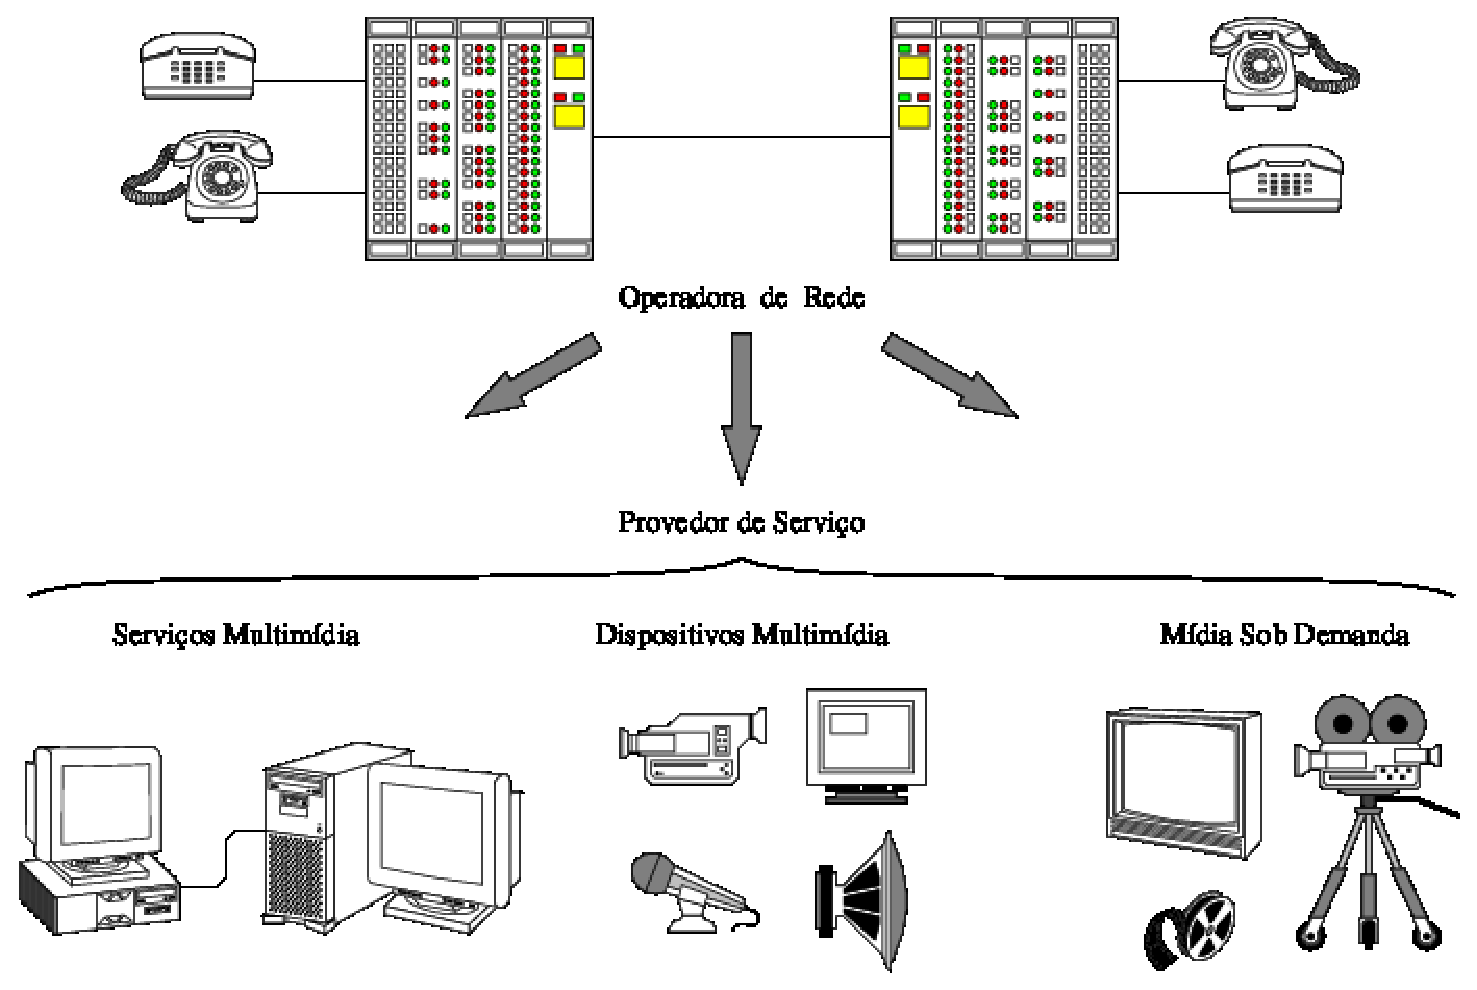
\includegraphics[width=0.6\textwidth]{figura1}%% Dimensões e localização
\fonte{\citet{Larsson2003}}%% Fonte
\end{figure}

Figuras em formato GIF, JPEG e BMP podem ser convertidas para o formato \gls{eps} por meio do aplicativo ``xv''. O ``xv'' não lista o formato \gls{eps} dentre aqueles que é capaz de manipular. Entretanto, selecionando-se o formato \textit{PostScript} e fornecendo-se a extensão \texttt{eps} ao nome do arquivo, o formato \gls{eps} é gerado.

O ambiente \texttt{picture} permite a programação de imagens diretamente no \gls{latex}\index{LaTeX@\latex}, conforme exemplo apresentado na \autoref{fig:figura2}.

\begin{figure}[htb]%% Ambiente figure
%\captionsetup{width=8cm}%% Largura da legenda
\caption{Exemplo de figura criada a partir do ambiente \texttt{picture}}%% Legenda
\label{fig:figura2}%% Rótulo
\setlength{\unitlength}{1cm}%% Unidade de comprimento
\begin{picture}(8,5)(-4,-2.5)%% Ambiente picture
\put(-4,0){\vector(1,0){8}}
\put(3.75,-0.25){$\chi$}
\put(0,-2.5){\vector(0,1){5}}
\multiput(-4,1)(0.4,0){20}{\line(1,0){0.2}}
\multiput(-4,-1)(0.4,0){20}{\line(1,0){0.2}}
\put(0.25,2.25){$\beta \equiv v / c = \tanh \chi$}
\qbezier(0,0)(0.8853,0.8853)(2,0.9640)
\qbezier(0,0)(-0.8853,-0.8853)(-2,-0.9640)
\end{picture}
\fonte{}%% Fonte
\end{figure}

%% Título e rótulo de seção (rótulos não devem conter caracteres especiais, acentuados ou cedilha)
\subsection{Fotografias}\label{sec:fotografias}

Um exemplo deste tipo de ilustração é apresentado na \autoref{foto:foto1}.

\begin{photograph}[htb]%% Ambiente photograph
%\captionsetup{width=0.6\textwidth}%% Largura da legenda
\caption{Camaleão pantera fotografado por Joel Sartore, National Geographic}%% Legenda
\label{foto:foto1}%% Rótulo
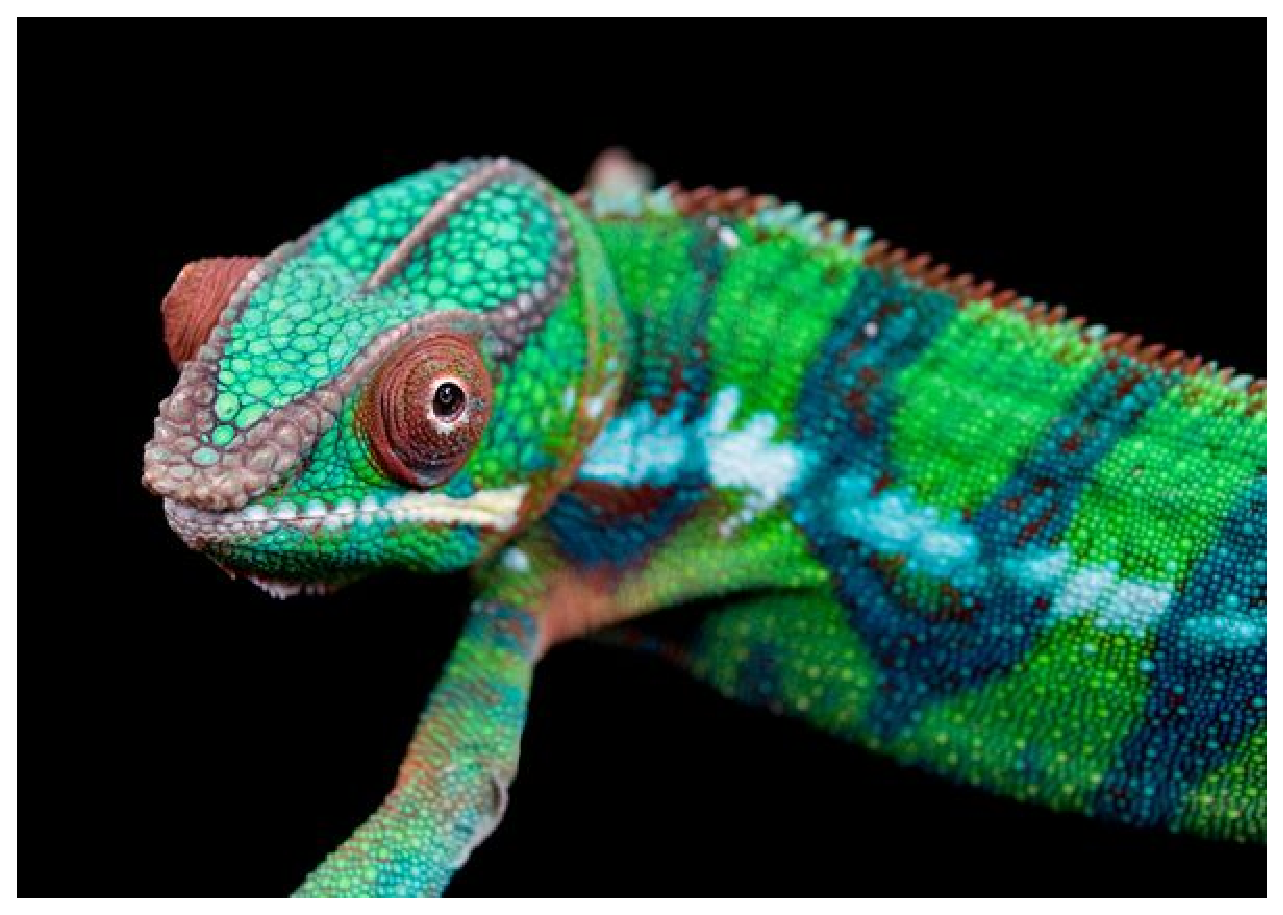
\includegraphics[width=0.95\textwidth]{foto1}%% Dimensões e localização
\fonte{\citet{Sartore2013}}%% Fonte
\end{photograph}

Outro exemplo deste tipo de ilustração é apresentado na \autoref{foto:foto2}.

\begin{photograph}[htb]%% Ambiente photograph
\captionsetup{width=0.6\textwidth}%% Largura da legenda
\caption{Fotografia da erupção vulcânica em 1982 do Galungung, Indonésia (com descargas de raios), produzida pelo Serviço Geológico dos Estados Unidos da América}%% Legenda
\label{foto:foto2}%% Rótulo
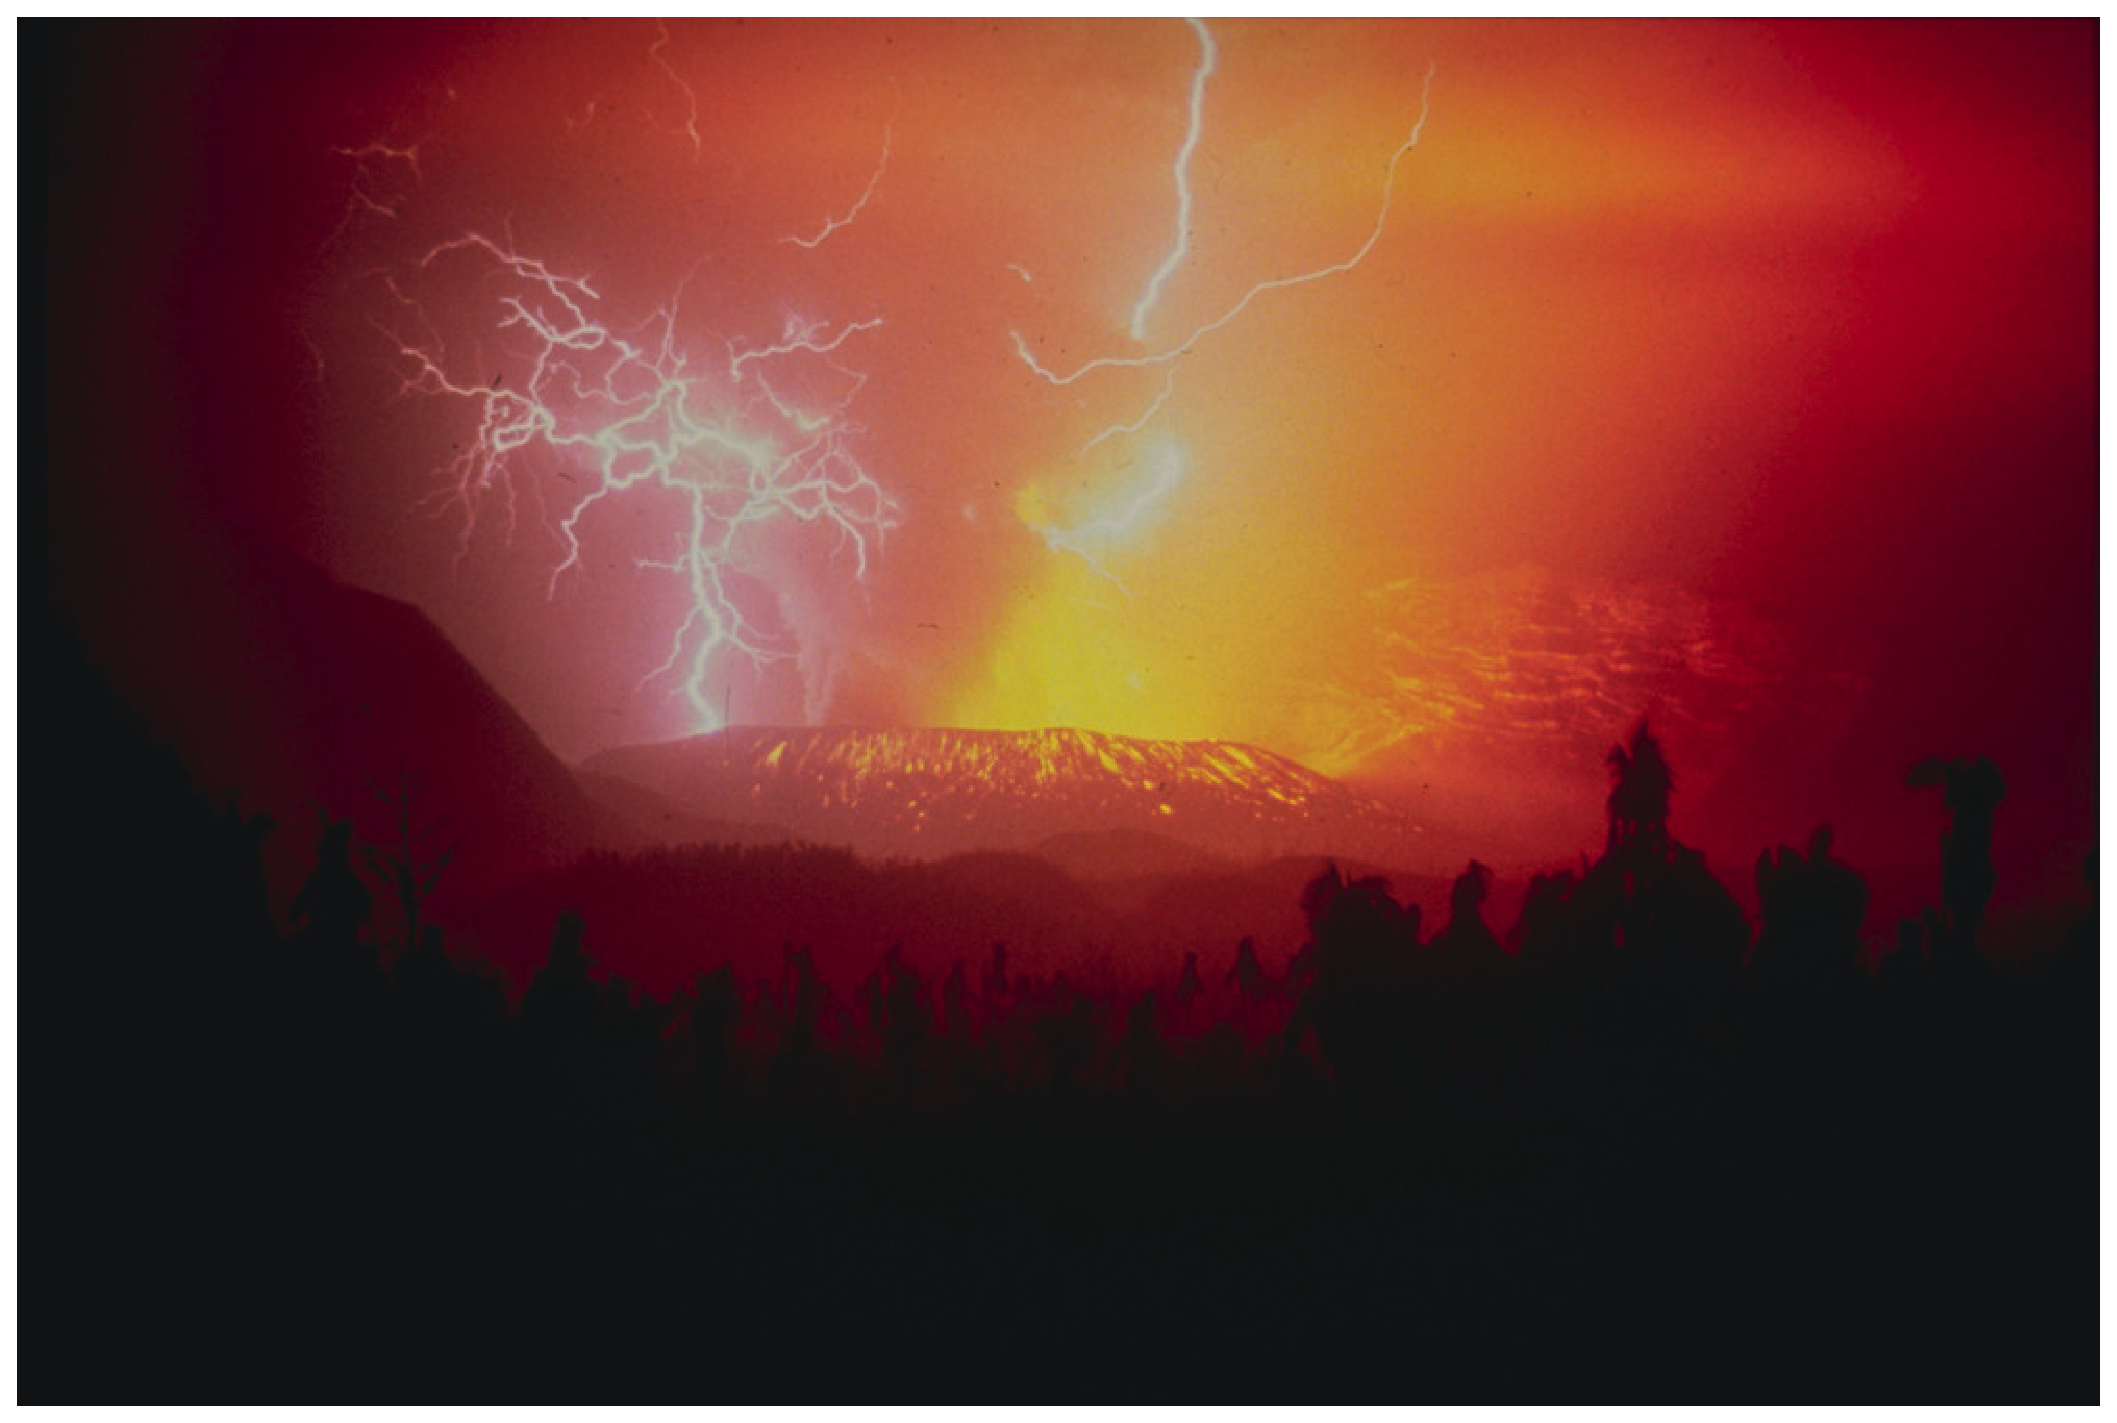
\includegraphics[width=0.6\textwidth]{foto2}%% Dimensões e localização
\fonte{\citet{Hadian1982}}%% Fonte
\end{photograph}

%% Título e rótulo de seção (rótulos não devem conter caracteres especiais, acentuados ou cedilha)
\subsection{Gráficos}\label{sec:graficos}

Gráficos são gerados com aplicativos capazes de exportar nos formatos \gls{ps} ou \gls{eps}. A ferramenta ``gnuplot'' é uma das mais utilizadas para a geração de gráficos (\url{http://www.gnuplot.info/}). Uma vez no formato \gls{eps}, gráficos são inseridos no texto tal como figuras, como pode ser observado no \autoref{gra:grafico1}.

\begin{graph}[htb]%% Ambiente graph
%\captionsetup{width=0.6\textwidth}%% Largura da legenda
\caption{Exemplo de gráfico produzido em ``gnuplot''}%% Legenda
\label{gra:grafico1}%% Rótulo
\includegraphics[width=0.6\textwidth]{grafico1}%% Dimensões e localização
\fonte{\citet{Faina2001}}%% Fonte
\end{graph}

No \autoref{gra:grafico2} é apresentado um exemplo de gráfico produzido em ``Excel''.

\begin{graph}[htb]%% Ambiente graph
%\captionsetup{width=0.6\textwidth}%% Largura da legenda
\caption{Exemplo de gráfico produzido em ``Excel''}%% Legenda
\label{gra:grafico2}%% Rótulo
\includegraphics[width=0.6\textwidth]{grafico2}%% Dimensões e localização
\fonte{\citeonline[p. 24]{Araujo2012}}%% Fonte
\end{graph}

O ambiente \texttt{minipage} pode ser usado para inserir textos ou outros elementos em quadros com tamanhos e posições controladas, conforme exemplos apresentados no \autoref{gra:minipagegrafico1} e no \autoref{gra:minipagegrafico2}.

\begin{graph}[htb]%% Ambiente graph
\begin{minipage}[t]{0.395\textwidth}%% Ambiente minipage
\centering%% Centralizado
%\captionsetup{width=0.85\textwidth}%% Largura da legenda
\caption{Gráfico 1 do ambiente \texttt{minipage}}%% Legenda
\label{gra:minipagegrafico1}%% Rótulo
\includegraphics[width=0.85\textwidth]{grafico1}%% Dimensões e localização
\fonte{\citet{Faina2001}}%% Fonte
\end{minipage}
\hfill
\begin{minipage}[t]{0.595\textwidth}%% Ambiente minipage
\centering%% Centralizado
\captionsetup{width=0.95\textwidth}%% Largura da legenda
\caption{Gráfico 2 do ambiente \texttt{minipage}}%% Legenda
\label{gra:minipagegrafico2}%% Rótulo
\includegraphics[width=0.95\textwidth]{grafico2}%% Dimensões e localização
\fonte{\citeonline[p. 24]{Araujo2012}}%% Fonte
\end{minipage}
\label{gra:minipagegraficos}
\end{graph}

%% Título e rótulo de seção (rótulos não devem conter caracteres especiais, acentuados ou cedilha)
\subsection{Quadros}\label{sec:quadros}

Um exemplo deste tipo de ilustração é apresentado no \autoref{quad:quadro1}.

\begin{tabframed}[htb]%% Ambiente tabframed
%\captionsetup{width=0.5\textwidth}%% Largura da legenda
\caption{Compostos orgânicos: fórmulas estruturais e principais classes}%% Legenda
\label{quad:quadro1}%% Rótulo
\includegraphics[width=0.5\textwidth]{quadro1}%% Dimensões e localização
\fonte{\citet{daSilva2009}}%% Fonte
\end{tabframed}

Outro exemplo deste tipo de ilustração é apresentado no \autoref{quad:quadro2}.

\begin{tabframed}[htb]%% Ambiente tabframed
%\captionsetup{width=0.7\textwidth}%% Largura da legenda
\caption{Modelos de maturidade para a gestão da cadeia de suprimentos}%% Legenda
\label{quad:quadro2}%% Rótulo
\includegraphics[width=0.7\textwidth]{quadro2}%% Dimensões e localização
\fonte{\citet{Frederico2012}}%% Fonte
\end{tabframed}

Os quadros não devem ser chamados de tabelas, uma vez que se diferenciam destas por apresentarem as laterais fechadas e o conteúdo não numérico.

%% Título e rótulo de seção (rótulos não devem conter caracteres especiais, acentuados ou cedilha)
\section{Tabelas}\label{sec:tabelas}

Tabelas são construídas com comandos próprios do \gls{latex}\index{LaTeX@\latex}. Por exemplo, a \autoref{tab:tabela1} foi construída desta forma.

\begin{table}[htb]%% Ambiente table
\caption{Primeiro exemplo de tabela com uma legenda contendo um texto muito longo que pode ocupar mais de uma linha}%% Legenda
\label{tab:tabela1}%% Rótulo
\begin{tabularx}{\textwidth}{@{\extracolsep{\fill}}llll}%% Ambiente tabularx
\toprule
$\bsym{L}$ & $\bsym{L^2}$ & $\bsym{L^3}$ & $\bsym{L^4}$ \\
\SI{}{[m]} & \SI{}{[m^2]} & \SI{}{[m^3]} & \SI{}{[m^4]} \\ \midrule
1          & 1            & 1            & 1            \\
2          & 4            & 8            & 16           \\
3          & 9            & 27           & 81           \\
4          & 16           & 64           & 256          \\
5          & 25           & 125          & 625          \\ \bottomrule
\end{tabularx}
\fonte{}%% Fonte
\end{table}

A \autoref{tab:tabela2} é um exemplo de tabela que ocupa mais de uma página e que foi construída pelo \gls{latex}\index{LaTeX@\latex} utilizando o pacote \texttt{longtable}.

\begin{longtable}{@{\extracolsep{\fill}}lll}%% Ambiente longtable
\caption{Possíveis tríplices para grade altamente variável\label{tab:tabela2}} \\%% Legenda e rótulo
\toprule
\textbf{Tempo (s)} & \textbf{Tríplice escolhida} & \textbf{Outras possíveis tríplices} \\
\midrule
\endfirsthead%% Encerra cabeçalho da primeira página
\caption[]{Possíveis tríplices para grade altamente variável} \\%% Legenda
\multicolumn{3}{r}{\textbf{(continuação)}} \\
\toprule
\textbf{Tempo (s)} & \textbf{Tríplice escolhida} & \textbf{Outras possíveis tríplices} \\
\midrule
\endhead%% Encerra cabeçalho das demais páginas
\midrule
\multicolumn{3}{r}{\textbf{(continua)}} \\
\endfoot%% Encerra rodapé das demais páginas
\bottomrule
\\[-0.5\linha]
\caption*{\nomefonte: Adaptado de \citet{Smallen2014}.} \\
\endlastfoot%% Encerra rodapé da última página
0      & (1, 11, 13725) & (1, 12, 10980), (1, 13, 8235), (2, 2, 0), (3, 1, 0) \\
2745   & (1, 12, 10980) & (1, 13, 8235), (2, 2, 0), (2, 3, 0), (3, 1, 0)      \\
5490   & (1, 12, 13725) & (2, 2, 2745), (2, 3, 0), (3, 1, 0)                  \\
8235   & (1, 12, 16470) & (1, 13, 13725), (2, 2, 2745), (2, 3, 0), (3, 1, 0)  \\
10980  & (1, 12, 16470) & (1, 13, 13725), (2, 2, 2745), (2, 3, 0), (3, 1, 0)  \\
13725  & (1, 12, 16470) & (1, 13, 13725), (2, 2, 2745), (2, 3, 0), (3, 1, 0)  \\
16470  & (1, 13, 16470) & (2, 2, 2745), (2, 3, 0), (3, 1, 0)                  \\
19215  & (1, 12, 16470) & (1, 13, 13725), (2, 2, 2745), (2, 3, 0), (3, 1, 0)  \\
21960  & (1, 12, 16470) & (1, 13, 13725), (2, 2, 2745), (2, 3, 0), (3, 1, 0)  \\
24705  & (1, 12, 16470) & (1, 13, 13725), (2, 2, 2745), (2, 3, 0), (3, 1, 0)  \\
27450  & (1, 12, 16470) & (1, 13, 13725), (2, 2, 2745), (2, 3, 0), (3, 1, 0)  \\
30195  & (2, 2, 2745)   & (2, 3, 0), (3, 1, 0)                                \\
32940  & (1, 13, 16470) & (2, 2, 2745), (2, 3, 0), (3, 1, 0)                  \\
35685  & (1, 13, 13725) & (2, 2, 2745), (2, 3, 0), (3, 1, 0)                  \\
38430  & (1, 13, 10980) & (2, 2, 2745), (2, 3, 0), (3, 1, 0)                  \\
41175  & (1, 12, 13725) & (1, 13, 10980), (2, 2, 2745), (2, 3, 0), (3, 1, 0)  \\
43920  & (1, 13, 10980) & (2, 2, 2745), (2, 3, 0), (3, 1, 0)                  \\
46665  & (2, 2, 2745)   & (2, 3, 0), (3, 1, 0)                                \\
49410  & (2, 2, 2745)   & (2, 3, 0), (3, 1, 0)                                \\
52155  & (1, 12, 16470) & (1, 13, 13725), (2, 2, 2745), (2, 3, 0), (3, 1, 0)  \\
54900  & (1, 13, 13725) & (2, 2, 2745), (2, 3, 0), (3, 1, 0)                  \\
57645  & (1, 13, 13725) & (2, 2, 2745), (2, 3, 0), (3, 1, 0)                  \\
60390  & (1, 12, 13725) & (2, 2, 2745), (2, 3, 0), (3, 1, 0)                  \\
63135  & (1, 13, 16470) & (2, 2, 2745), (2, 3, 0), (3, 1, 0)                  \\
65880  & (1, 13, 16470) & (2, 2, 2745), (2, 3, 0), (3, 1, 0)                  \\
68625  & (2, 2, 2745)   & (2, 3, 0), (3, 1, 0)                                \\
71370  & (1, 13, 13725) & (2, 2, 2745), (2, 3, 0), (3, 1, 0)                  \\
74115  & (1, 12, 13725) & (2, 2, 2745), (2, 3, 0), (3, 1, 0)                  \\
76860  & (1, 13, 13725) & (2, 2, 2745), (2, 3, 0), (3, 1, 0)                  \\
79605  & (1, 13, 13725) & (2, 2, 2745), (2, 3, 0), (3, 1, 0)                  \\
82350  & (1, 12, 13725) & (2, 2, 2745), (2, 3, 0), (3, 1, 0)                  \\
85095  & (1, 12, 13725) & (1, 13, 10980), (2, 2, 2745), (2, 3, 0), (3, 1, 0)  \\
87840  & (1, 13, 16470) & (2, 2, 2745), (2, 3, 0), (3, 1, 0)                  \\
90585  & (1, 13, 16470) & (2, 2, 2745), (2, 3, 0), (3, 1, 0)                  \\
93330  & (1, 13, 13725) & (2, 2, 2745), (2, 3, 0), (3, 1, 0)                  \\
96075  & (1, 13, 16470) & (2, 2, 2745), (2, 3, 0), (3, 1, 0)                  \\
98820  & (1, 13, 16470) & (2, 2, 2745), (2, 3, 0), (3, 1, 0)                  \\
101565 & (1, 13, 13725) & (2, 2, 2745), (2, 3, 0), (3, 1, 0)                  \\
104310 & (1, 13, 16470) & (2, 2, 2745), (2, 3, 0), (3, 1, 0)                  \\
107055 & (1, 13, 13725) & (2, 2, 2745), (2, 3, 0), (3, 1, 0)                  \\
109800 & (1, 13, 13725) & (2, 2, 2745), (2, 3, 0), (3, 1, 0)                  \\
112545 & (1, 12, 16470) & (1, 13, 13725), (2, 2, 2745), (2, 3, 0), (3, 1, 0)  \\
115290 & (1, 13, 16470) & (2, 2, 2745), (2, 3, 0), (3, 1, 0)                  \\
118035 & (1, 13, 13725) & (2, 2, 2745), (2, 3, 0), (3, 1, 0)                  \\
120780 & (1, 13, 16470) & (2, 2, 2745), (2, 3, 0), (3, 1, 0)                  \\
123525 & (1, 13, 13725) & (2, 2, 2745), (2, 3, 0), (3, 1, 0)                  \\
126270 & (1, 12, 16470) & (1, 13, 13725), (2, 2, 2745), (2, 3, 0), (3, 1, 0)  \\
129015 & (2, 2, 2745)   & (2, 3, 0), (3, 1, 0)                                \\
131760 & (2, 2, 2745)   & (2, 3, 0), (3, 1, 0)                                \\
134505 & (1, 13, 16470) & (2, 2, 2745), (2, 3, 0), (3, 1, 0)                  \\
137250 & (1, 13, 13725) & (2, 2, 2745), (2, 3, 0), (3, 1, 0)                  \\
139995 & (2, 2, 2745)   & (2, 3, 0), (3, 1, 0)                                \\
142740 & (2, 2, 2745)   & (2, 3, 0), (3, 1, 0)                                \\
145485 & (1, 12, 16470) & (1, 13, 13725), (2, 2, 2745), (2, 3, 0), (3, 1, 0)  \\
148230 & (2, 2, 2745)   & (2, 3, 0), (3, 1, 0)                                \\
150975 & (1, 13, 16470) & (2, 2, 2745), (2, 3, 0), (3, 1, 0)                  \\
153720 & (1, 12, 13725) & (2, 2, 2745), (2, 3, 0), (3, 1, 0)                  \\
156465 & (1, 13, 13725) & (2, 2, 2745), (2, 3, 0), (3, 1, 0)                  \\
159210 & (1, 13, 13725) & (2, 2, 2745), (2, 3, 0), (3, 1, 0)                  \\
161955 & (1, 13, 16470) & (2, 2, 2745), (2, 3, 0), (3, 1, 0)                  \\
164700 & (1, 13, 13725) & (2, 2, 2745), (2, 3, 0), (3, 1, 0)                  \\
\end{longtable}

Tabelas criadas em planilhas do ``Excel'' podem ser convertidas em tabelas \gls{latex}\index{LaTeX@\latex} utilizando o suplemento ``Excel-to-LaTeX'', disponível em \url{http://www.ctan.org/pkg/excel2latex}.

\textbf{Atenção!} É fortemente recomendável que as tabelas sejam criadas através de ferramentas \textit{online} ou \textit{plugins} do LibreOffice ou Microsoft Office, pois assim o trabalho de criar as tabelas fica bem mais fácil. Seguem \textit{links} de sítios \textit{online} que permitem criar tais tabelas, depois só é necessário copiar o código da tabela gerada por esses sítios para o texto do trabalho em \gls{latex}\index{LaTeX@\latex}:
\begin{itemize}
    \item \url{https://www.tablesgenerator.com/};
    \item \url{https://www.latex-tables.com/};
    \item \url{https://tableconvert.com/latex-generator};
    \item É possível buscar por outras na Internet através de termos de busca como ``latex table online'' ou ``latex criar tabela online''.
\end{itemize}

%% Título e rótulo de seção (rótulos não devem conter caracteres especiais, acentuados ou cedilha)
\section{Abreviaturas e siglas}\label{sec:acronimos}

\gls{latex}\index{LaTeX@\latex} gera automaticamente a lista de abreviaturas e siglaspor meio do pacote \texttt{glossaries}. As abreviaturas e siglas devem ser definidos no arquivo \texttt{entradas-acronimos.tex}, no diretório ``PreTexto'', com os comandos:

\begin{SingleSpacing}%% Ambiente SingleSpacing
\begin{verbatim}
\abreviatura{rótulo}{representação}{definição}
\sigla{rótulo}{representação}{definição}
\acronimo{rótulo}{representação}{definição}
\end{verbatim}
\end{SingleSpacing}

Para que a abreviatura ou sigla seja apresentada em alguma parte do texto do documento use o comando \verb|\gls{rótulo}|, por exemplo, as abreviaturas \gls{art.}, \gls{cap.} e \gls{sec.} foram geradas pelos comandos \verb|\gls{art.}, \gls{cap.} e \gls{sec.}|, respectivamente. Mais detalhes dos comandos do pacote \texttt{glossaries} podem ser encontrados em: \url{http://mirrors.ctan.org/macros/latex/contrib/glossaries/glossaries-user.pdf}.

Outra opção para gerar a lista de abreviaturas e siglas é por meio da edição manual do arquivo \texttt{lista-acronimos.tex} no diretório ``PreTexto''.

%% Título e rótulo de seção (rótulos não devem conter caracteres especiais, acentuados ou cedilha)
\section{Símbolos}\label{sec:simbolos}

\gls{latex}\index{LaTeX@\latex} gera automaticamente a lista de símbolos por meio do pacote \texttt{nomencl}. Ao redigir um símbolo pela primeira vez em qualquer parte do texto com o comando \verb|\nomenclature[prefixo]{símbolo}{descrição \nomunit{unidade}}|, é gerada uma entrada para a lista de símbolos. Veja exemplos deste comando no arquivo fonte deste capítulo. Os elementos da lista de símbolos são agrupados a depender da primeira letra atribuída ao prefixo e classificadas em:

\begin{itemize}%% Lista de itens
\item Letras Latinas.
\item Letras Gregas.
\item Sobrescritos.
\item Subscritos.
\item Notações.
\end{itemize}

Outra opção ao comando \verb|\nomenclature| é o uso dos atalhos:

\begin{SingleSpacing}%% Ambiente SingleSpacing
\begin{verbatim}
\letralatina{prefixo}{símbolo}{descrição}{unidade}
\letragrega{prefixo}{símbolo}{descrição}{unidade}
\sobrescrito{prefixo}{símbolo}{descrição}{unidade}
\subscrito{prefixo}{símbolo}{descrição}{unidade}
\notacao{prefixo}{símbolo}{descrição}{unidade}
\end{verbatim}
\end{SingleSpacing}

\noindent Neste caso a atribuição da primeira letra do prefixo pode ser desprezada.

%% Letras Latinas [A]
\nomenclature[AA]{$A$}{Área \nomunit{m^2}}%%
\letralatina{L}{L}{Comprimento}{m}%%
\letralatina{R}{R}{Raio}{m}%%
%% Letras Gregas [B]
\nomenclature[Bmu]{$\mu$}{Viscosidade dinâmica \nomunit{kg/(m.s)}}%%
\letragrega{nu}{\nu}{Viscosidade cinemática}{m^2/s}%%
\letragrega{pi}{\pi}{Pi (constante circular)}{rad}%%
\letragrega{rho}{\rho}{Massa específica}{kg/m^3}%%
\letragrega{sigma}{\sigma}{Tensão superficial}{N/m}%%
%% Sobrescritos [C]
\nomenclature[C+]{$+$}{Passo de tempo posterior}%%
\sobrescrito{-}{-}{Passo de tempo anterior}{}%%
\sobrescrito{0}{0}{Valor inicial}{}%%
%% Subscritos [D]
\nomenclature[DG]{$G$}{Fase gasosa}%%
\subscrito{L}{L}{Fase líquida}{}%%
\subscrito{S}{S}{Fase sólida}{}%%
%% Notações [E]
\nomenclature[EPsi_1]{$\overline{\Psi}$}{Média temporal}%%
\notacao{Psi_2}{\langle \Psi \rangle}{Média na seção transversal}{}%%
\notacao{Psi_3}{\langle\langle \Psi \rangle\rangle}{Média na seção transversal ponderada}{}%%

Mais detalhes dos comandos do pacote \texttt{nomencl} podem ser encontrados em: \url{http://tug.ctan.org/tex-archive/macros/latex/contrib/nomencl/nomencl.pdf}.

Outra opção para gerar a lista de símbolos é por meio da edição manual do arquivo \texttt{lista-simbolos.tex} no diretório ``PreTexto''.

%% Título e rótulo de seção (rótulos não devem conter caracteres especiais, acentuados ou cedilha)
\section{Inclusão de outros arquivos}\label{sec:inclusao}

É uma boa prática dividir o seu documento em diversos arquivos, e não apenas escrever tudo em um único. Esse recurso foi utilizado neste documento (veja \texttt{utfprpb.tex}). Para incluir diferentes arquivos em um arquivo principal, de modo que cada arquivo incluído fique em uma página diferente, utilize o comando:

\begin{SingleSpacing}%% Ambiente SingleSpacing
\begin{verbatim}
\include{documento-a-ser-incluido} %% Sem a extensão .tex
\end{verbatim}
\end{SingleSpacing}

Para incluir documentos sem quebra de páginas, utilize:

\begin{SingleSpacing}%% Ambiente SingleSpacing
\begin{verbatim}
\input{documento-a-ser-incluido}   %% Sem a extensão .tex
\end{verbatim}
\end{SingleSpacing}

%% Título e rótulo de seção (rótulos não devem conter caracteres especiais, acentuados ou cedilha)
\section{Referências}\label{sec:referencias}

A formatação das referências bibliográficas conforme as regras da \gls{abnt}\index{ABNT} são um dos principais objetivos do \gls{abntex2}\index{abnTeX2@\abnTeX}. Consulte os manuais \citeonline{abnTeX2:2013Cite} e \citeonline{abnTeX2:2013CiteAlf} para obter informações sobre sua utilização.

%% Título e rótulo de seção (rótulos não devem conter caracteres especiais, acentuados ou cedilha)
%\subsection{Acentuação de referências bibliográficas}\label{sec:acentuacaodereferencias}

Normalmente não há problemas em usar caracteres acentuados em arquivos bibliográficos (extensão \texttt{bib}). Porém, como as regras da \gls{abnt}\index{ABNT} fazem uso quase abusivo da conversão para letras maiúsculas, é preciso observar o modo como se escreve os nomes dos autores e/ou editores. No \autoref{quad:quadro3} você encontra alguns exemplos das conversões mais importantes. A regra geral é sempre usar a acentuação neste modo quando houver conversão para letras maiúsculas.

\begin{tabframed}[htb]%% Ambiente tabframed
%\captionsetup{width=0.5\textwidth}%% Largura da legenda
\caption{Conversão de acentuação em arquivos \texttt{bibtex}}%% Legenda
\label{quad:quadro3}%% Rótulo
\begin{tabular}{|*{2}{p{0.25\textwidth-\columnsep}|}}%% Ambiente tabular
\hline
\textbf{Acento}   & \textbf{Comando}                       \\ \hline
{\'a} {\`a} {\~a} & \verb|{\'a}| \verb|{\`a}| \verb|{\~a}| \\ \hline
{\^e}             & \verb|{\^e}|                           \\ \hline
{\"u}             & \verb|{\"u}|                           \\ \hline
{\'\i}            & \verb|{\'\i}|                          \\ \hline
{\c{c}}           & \verb|{\c{c}}|                         \\ \hline
\end{tabular}
\fonte{}%% Fonte
\end{tabframed}

%% Título e rótulo de seção (rótulos não devem conter caracteres especiais, acentuados ou cedilha)
\section{Glossário}\label{sec:glossario}

Você pode definir as entradas do glossário no início do texto. Recomenda-se o uso de um arquivo separado a ser inserido ainda no preâmbulo do documento, como por exemplo o arquivo \texttt{entradas-glossario.tex} no diretório ``PosTexto'' do presente documento. Veja orientações sobre inclusão de arquivos na \autoref{sec:inclusao}.

`O \gls{abntex2} é \glsdesc*{abntex2}' é um exemplo de termo definido no glossário e usado no decorrer do texto, bem como:

\begin{citacao}%% Ambiente citacao
Esta frase usa a palavra \gls{componente} e o plural de \glspl{filho}, ambas definidas no glossário como filhas da entrada \gls{pai}. \Gls{equilibrio} exemplifica o uso de um termo no início da frase. O software \gls{abntex2}\index{abnTeX2@\abnTeX} é escrito em \gls{latex}\index{LaTeX@\latex}, que é definido no glossário como `\glsdesc*{latex}'.
\end{citacao}

A frase da citação direta acima foi produzida com:

\begin{SingleSpacing}%% Ambiente SingleSpacing
\begin{verbatim}
Esta frase usa a palavra \gls{componente} e o plural de
\glspl{filho}, ambas definidas no glossário como filhas da
entrada \gls{pai}. \Gls{equilibrio} exemplifica o uso de um
termo no início da frase. O software \gls{abntex2} é
escrito em \gls{latex}, que é definido no glossário como
`\glsdesc*{latex}'.
\end{verbatim}
\end{SingleSpacing}

A impressão efetiva do glossário é dada com:

\begin{SingleSpacing}%% Ambiente SingleSpacing
\begin{verbatim}
\printglossaries
\end{verbatim}
\end{SingleSpacing}

A impressão do glossário incorpora o número das páginas em que as entradas foram citadas. Isso pode ser removido adicionando-se a opção \texttt{nonumberlist} em:

\begin{SingleSpacing}%% Ambiente SingleSpacing
\begin{verbatim}
\usepackage[nonumberlist, style=index]{glossaries}
\end{verbatim}
\end{SingleSpacing}

%% Título e rótulo de seção (rótulos não devem conter caracteres especiais, acentuados ou cedilha)
\section{Apêndices e anexos}\label{sec:apendiceseanexos}

Apêndices e anexos podem ser inseridos no documento, logo após o glossário, por meio da inclusão de arquivos, como por exemplo, os arquivos fontes \texttt{apendicea.tex}, \texttt{apendiceb.tex}, \texttt{anexoa.tex} e \texttt{anexob.tex}, presentes no diretório ``PosTexto'' deste projeto, são utilizados para gerar o \autoref{cap:apendicea}, o \autoref{cap:apendiceb}, o \autoref{cap:anexoa} e o \autoref{cap:anexob}, respectivamente. Veja orientações sobre inclusão de arquivos na \autoref{sec:inclusao}.

%% Título e rótulo de seção (rótulos não devem conter caracteres especiais, acentuados ou cedilha)
\section{Índice remissivo}\label{sec:indice}

Palavras podem ser indexadas no índice remissivo por meio do comando \verb|\index{palavra a ser indexada}|. Existem vários exemplos do uso deste comando no arquivo fonte deste capítulo. Por exemplo o comando \verb|\index{Windows}| é utilizado para indexar a palavra Windows\index{Windows} no índice remissivo.

%% Título e rótulo de seção (rótulos não devem conter caracteres especiais, acentuados ou cedilha)
\section{Compilação do documento latex}\label{sec:compilar}\index{LaTeX@\latex}

Geralmente os editores \gls{latex}\index{LaTeX@\latex}, como o TeXlipse\index{TeXlipse}\footnote{Disponível em \url{http://texlipse.sourceforge.net/}.}, o Texmaker\index{Texmaker}\footnote{Disponível em \url{http://www.xm1math.net/texmaker/}.}, entre outros, compilam os documentos automaticamente ou após configuração, de modo que você não precisa se preocupar com isto.

No entanto, você pode compilar os documentos \gls{latex}\index{LaTeX@\latex} usando os seguintes comandos, que devem ser digitados no \textit{Prompt} de comandos do Windows\index{Windows} ou no terminal do Mac\index{Mac} ou do Linux\index{Linux}:

\begin{SingleSpacing}%% Ambiente SingleSpacing
\begin{verbatim}
latex <mainfile>.tex
bibtex <mainfile>
latex <mainfile>.tex
latex <mainfile>.tex
dvips <dvips configs> <mainfile>.dvi -o <mainfile>.ps
ps2pdf <mainfile>.ps <mainfile>.pdf
\end{verbatim}
\end{SingleSpacing}

\noindent se todas as figuras no seu documento estão no formato \gls{eps}, ou então, usando os seguintes comandos:

\begin{SingleSpacing}%% Ambiente SingleSpacing
\begin{verbatim}
pdflatex <mainfile>.tex
bibtex <mainfile>
pdflatex <mainfile>.tex
pdflatex <mainfile>.tex
\end{verbatim}
\end{SingleSpacing}

\noindent se todas as figuras no seu documento estão no \gls{pdf}, ou em formatos comuns de imagens (BMP, GIF, JPG ou PNG).

%% Título e rótulo de seção (rótulos não devem conter caracteres especiais, acentuados ou cedilha)
\subsection{Problemas de compilação}\label{sec:problemas}

O \gls{utfprpbtex}\index{UTFPRPBTeX@\utfprtex} foi configurado e testado para compilar documentos \gls{latex}\index{LaTeX@\latex} sem problemas, mas por se tratar de uma linguagem de programação (para editoração) está sujeita a \textit{bugs} como qualquer outra linguagem. Além disto, o \gls{utfprpbtex}\index{UTFPRPBTeX@\utfprtex} é baseado em outras classes de documento e também utiliza uma quantidade considerável de pacotes que podem ter incompatibilidades. Portanto, alguns cuidados devem ser tomados quando se trabalha com \gls{latex}\index{LaTeX@\latex}, principalmente para novos usuários:

\begin{itemize}%% Lista de itens
\item Os comandos devem ser corretamente finalizados, ou seja, deve-se verificar a abertura e fechamento dos colchetes e chaves: \verb|\comando[opções]{argumentos}|. Alguns comandos não necessitam disto, por exemplo \verb|\comando|, mas as vezes torna-se necessário colocar uma barra invertida, \verb|\|, ou chaves, \verb|{}|, após o comando para gerar um espaço com o texto na sequência: \verb|\comando\ texto na sequência do comando| ou \verb|\comando{} texto na sequência do comando|.
\item Os ambientes devem ser corretamente finalizados, ou seja, deve-se verificar a abertura e fechamento dos ambientes: \verb|\begin{ambiente} ... \end{ambiente}|.
\item Os caracteres especiais devem ser precedidos de barra invertida quando se deseja imprimí-los no texto: \verb|\$ \& \% \# \_ \{ \}| resulta em \$ \& \% \# \_ \{ \}. Do contrário, não serão impressos e executarão comandos específicos do \gls{latex}\index{LaTeX@\latex}.
\item Os textos copiados de outros arquivos (\texttt{*.doc}, \texttt{*.html}, \texttt{*.pdf}, etc.) para os arquivos fonte do \gls{latex}\index{LaTeX@\latex} (\texttt{*.tex}, \texttt{*.bib}, etc.) devem ter a mesma codificação de caracteres (\texttt{UTF8}). Do contrário, alguns caracteres não serão devidamente impressos ou causarão erro, por exemplo, o hífen e os caracteres acentuados.
\item Os nomes de arquivos carregados no modelo (arquivos fontes, figuras, etc.) não devem conter caracteres especiais ou acentuados: \verb|capitulo1.tex| ao invés de \verb|capitulo_1.tex|. Esta regra também se aplica aos rótulos: \verb|\label{cap:capitulo1}| ao invés de \verb|\label{cap:capitulo_1}|.
\end{itemize}

Outras dicas de uso dos comandos do \gls{latex}\index{LaTeX@\latex} podem ser encontradas em diversos materiais de referência disponíveis na Internet, por exemplo: \url{http://en.wikibooks.org/wiki/LaTeX}, \url{http://repositorios.cpai.unb.br/ctan/info/lshort/portuguese-BR/lshortBR.pdf}, entre outros.

%% Licença utilizada no trabalho da UTFPR
\section{Licença}\label{sec:licenca}

De acordo com a Resolução Conjunta \href{https://sei.utfpr.edu.br/sei/publicacoes/controlador_publicacoes.php?acao=publicacao_visualizar&id_documento=1811618&id_orgao_publicacao=0}{nº 01/2020 COGEP-COPPG}, os trabalhos de conclusão de curso da \gls{utfpr} devem adotar uma licença Creative Commons, sendo que o texto das possíveis licenças pode ser visto em: \url{https://creativecommons.org/licenses/?lang=pt_BR}.

Para facilitar a adoção dessas licenças o presente \textit{template} possui o comando \texttt{$\backslash$licenca\{\}}, disponível no arquivo \texttt{variaveis.tex} do \textit{template}. As possibilidades para este comando são:

\begin{itemize}
    \item \texttt{$\backslash$licenca\{ccby\}} - para usar a licença CC BY (está como padrão no \textit{template}); 
    \item \texttt{$\backslash$licenca\{ccbysa\}} - para usar a licença CC BY CA;
    \item \texttt{$\backslash$licenca\{ccbynd\}} - para usar a licença CC BY ND;
    \item \texttt{$\backslash$licenca\{ccbync\}} - para usar a licença CC BY NC;
    \item \texttt{$\backslash$licenca\{ccbyncsa\}} - para usar a licença CC BY NC SA;
    \item \texttt{$\backslash$licenca\{ccbyncnd\}} - para usar a licença CC BY NC ND;
    \item \texttt{$\backslash$licenca\{\}} - deixar em branco, neste caso não aparecerá nenhuma licença (não recomendável).
\end{itemize}

Então, converse com o orientador a respeito de qual licença utilizar, localize o comando \texttt{$\backslash$licenca\{\}} no arquivo \texttt{variaveis.tex} e deixe descomentado (sem o \texttt{\%} no inicio da linha) apenas a licença que será utilizada no trabalho. Atenção, tome o cuidado de não deixar mais de uma licença desabilitada e confira se a licença escolhida é a que está aparecendo na Folha de Rosto do trabalho.%% Comente para remover este item

%% Parte
% \part{Conclusão}%% Comente para remover este item

%% Capítulo
%%%% CAPÍTULO 5 - CONCLUSÕES E PERSPECTIVAS
%%
\chapter{Conclusão}\label{cap:conclusoeseperspectivas}

A finalidade principal deste trabalho foi desenvolver um multimedidor com comunicação \textit{wireless} de baixo custo, capaz de medir tensão e corrente simultaneamente. De maneira sucinta, pode-se concluir que a produção do protótipo e a prova de conceito sobre a sua funcionalidade foram um sucesso.

As especificações do \gls{ADC} e do microcontrolador são as de maior importância para o desenvolvimento de um protótipo com esta finalidade. Isto se deve às necessidades a serem atendidas ou o propósito do instrumento de medição a ser elaborado, como precisão e ranges de leitura, quais tipos de leitura serão feitas, a interface homem-máquina, velocidade de transmissão de dados, entre várias outras. Uma consideração de suma importância também é a compatibilidade entre estes componentes.

Para alcançar o objetivo de leitura paralela de tensão e corrente, foi necessário o desenvolvimento de um circuito isolado internamente, garantindo a integridade dos sinais e dos componentes do circuito. Isto se apresentou como um grande desafio quando se trata de baixo custo e a replicabilidade do protótipo desenvolvido, pois soluções já existentes são em grande maioria custosas e difíceis de se encontrar em mercados não especializados.

O desenvolvimento do \textit{firmware} é necessário para o funcionamento do equipamento como um todo. Este integra todo o resultado da pesquisa e possibilita a comunicação entre o ADC e a plataforma de tratamento de dados, que pode ser acessada por dispositivos externos como smartphones ou computadores, assim como deixa estruturada uma futura modularização. Isto fez este uma das partes mais críticas do projeto, assim como desafiadora.

É interessante pontuar que as leituras true RMS de multímetros comercias não necessariamente conseguiriam fazer a leitura corretamente quando se tem um circuito que gera sinais com componentes DC devido ao acoplamento AC utilizado por estes multímetros para realizar sua leitura. O protótipo neste trabalho desenvolvido não possui acoplamento AC e considera a onda pura para o cálculo, resultando em um valor mais condizente com a realidade.

Para fazer esta medida com um multímetro true RMS seria necessário fazer uma medida AC, uma DC e calcular o resultado final com a equação $RMS=sqrt(CArms^2+CC^2)$". Multímetros que dispõe tal utilidade são custosos monetáriamente, o que é uma vantagem para o desenvolvimento do protótipo neste trabalho proposto. 

Considerando as especificações adotadas para o protótipo, as tabelas \ref{tab:resultados-precis} e \ref{tab:resultados-func} demonstram os resultados obtidos, considerando todos os aspectos da pesquisa.

\begin{table}[!h]
    \centering
    \caption{Precisões solicitadas e resultados}
    \label{tab:resultados-precis}
    \begin{tabular}{ l l l l }
        \hline
        \textbf{Parâmetro} & \textbf{Precisão Solicitada} & \textbf{Precisão Atingida} & \textbf{Status}         \\ \hline
        Tensão (V)         & < 2\%                        & entre 0,47\% e 1,46\%      & Dentro de Especificação \\ 
        Tensão (mV)        & < 2\%                        & entre 31,47\% e 37,23\%    & Fora de Especificação   \\ 
        Corrente (A)       & < 5\%                        & 0,047\%                    & Dentro de Especificação \\ 
        Corrente (mA)      & < 5\%                        & 2,72\%                     & Dentro de Especificação  \\ 
        Corrente ($\mu$A)  & < 5\%                        & 2,51\%                     & Dentro de Especificação   \\ \hline
    \end{tabular}
    \fonte{}
\end{table}

\begin{table}[!h]
    \centering
    \caption{Implementação de funções de acordo com especificações}
    \label{tab:resultados-func}
    \begin{tabular}{ l l }
        \hline
        \textbf{Função}                                  & \textbf{Status} \\ \hline
        Leitura Simultânea de Tensão e Corrente True RMS & Implementado  \\ 
        Exibição de Formas de Onda de Tensão e Corrente  & Implementado  \\ 
        Cálculo de Potências Ativa, Reativa e Aparente   & Implementado  \\ 
        Cálculo do Fator de Potência                     & Implementado  \\ \hline
        Modularização e Leitura de Multiplas Fases       & Não Implementado  \\ \hline
    \end{tabular}
    \fonte{}
\end{table}

De acordo com as especificações de aspectos construtivos, foi adicionado um borne a mais para a corrente visto a necessidade de se trocar a entrada desta para leituras de A, mA e $\mu$A. A utilização de fontes internas isoladas foi atendida e o tipo de interface homem-máquina também foi atendido, se dando por smartphone ou computador.

Nota-se que o dispositivo também oferece a leitura da frequência do sinal a ser medido. Além disto, de acordo com o teste utilizando-se o circuito de Wheatstone, a leitura simultânea de sinais de corrente e tensão em partes diferentes do circuito sem interferências é provada.

Quanto aos resultados dos testes, nota-se que as especificações foram em sua grande maioria atendidas, exceto o range de mV, devido a uma má calibração de seus parâmetros. Este pode ser calibrado posteriormente por meio do firmware integrado ao dispositivo para o aperfeiçoamento da aquisição destes sinais e então sua leitura.

A funcionalidade de modularização não foi implementada nesta etapa devido à sua complexidade de implementação, por limitações de protocolos de comunicação \textit{wireless} atrelados à plataforma e o hardware escolhidos e também por limitações de tempo. 

Com isso, propõe-se para trabalhos futuros a implementação da modularidade do sistema e com isso a expansão e otimização do software e firmware.%% Comente para remover este item

%% Capítulos após este comando criam marcadores do pdf na raiz
% \phantompart%% Comente para remover este item


%% Formatação de páginas de elementos pós-textuais
\postextual%% Não comente esta linha

%% Arquivos de referências
\arquivosdereferencias{%% Arquivos bibtex sem a extensão .bib e separados por vírgula - Não comente esta linha
  %./PosTexto/exemplos-referencias,%% Arquivo de referências - Comente para remover este item
  main%% Arquivo de referências - Comente para remover este item
}%% Não comente esta linha

%% Glossário
% \incluirglossario %% Comente para remover este item

%% Arquivos de apêndices
\begin{arquivosdeapendices}%% Os arquivos de apêndices devem se incluídos neste ambiente - Não comente esta linha
    % \partapendices%% Página de início dos apêndices - adiciona uma página com o título Apêndices
    % \section{Acesso ao Circuito, Código e Modelo 3D}\label{sec:apendice-a}
  %   %% Capítulo de exemplo
   %%%% APÊNDICE A
%%
%% Texto ou documento elaborado pelo autor, a fim de complementar sua argumentação, sem prejuízo da unidade nuclear do trabalho.

%% Título e rótulo de apêndice (rótulos não devem conter caracteres especiais, acentuados ou cedilha)
\chapter{Título do Apêndice A com um Texto Muito Longo que Pode Ocupar Mais de uma Linha}\label{cap:apendicea}

Quando houver necessidade pode-se apresentar como apêndice documento(s) auxiliar(es) e/ou complementar(es) como: legislação, estatutos, gráficos, tabelas, etc. Os apêndices são enumerados com letras maiúsculas: \autoref{cap:apendicea}, \autoref{cap:apendiceb}, etc.

No \latex\ apêndices são editados como capítulos. O comando \verb|\appendix| faz com que todos os capítulos seguintes sejam considerados apêndices.

Apêndices complementam o texto principal da tese com informações para leitores com especial interesse no tema, devendo ser considerados leitura opcional, ou seja, o entendimento do texto principal da tese não deve exigir a leitura atenta dos apêndices.

Apêndices usualmente contemplam provas de teoremas, deduções de fórmulas matemáticas, diagramas esquemáticos, gráficos e trechos de código. Quanto a este último, código extenso não deve fazer parte da tese, mesmo como apêndice. O ideal é disponibilizar o código na Internet para os interessados em examiná-lo ou utilizá-lo.

%% Título e rótulo de seção (rótulos não devem conter caracteres especiais, acentuados ou cedilha)
%\section{Título da Seção Secundária do Apêndice B}\label{sec:secaoapendicea}

%Exemplo de seção secundária em apêndice (\autoref{sec:secaoapendicea} do \autoref{cap:apendicea}).

%% Título e rótulo de seção (rótulos não devem conter caracteres especiais, acentuados ou cedilha)
%\subsection{Título da Seção Terciária do Apêndice B}\label{subsec:subsecaoapendicea}

%Exemplo de seção terciária em apêndice (\autoref{subsec:subsecaoapendicea} do \autoref{cap:apendicea}).

%% Título e rótulo de seção (rótulos não devem conter caracteres especiais, acentuados ou cedilha)
%\subsubsection{Título da seção quaternária do Apêndice B}\label{subsubsec:subsubsecaoapendicea}

%Exemplo de seção quaternária em apêndice (\autoref{subsubsec:subsubsecaoapendicea} do \autoref{cap:apendicea}).

%% Título e rótulo de seção (rótulos não devem conter caracteres especiais, acentuados ou cedilha)
%\paragraph{Título da seção quinária do Apêndice B}\label{para:paragraphapendicea}

%Exemplo de seção quinária em apêndice (\autoref{para:paragraphapendicea} do \autoref{cap:apendicea}).
%% Apêndice - Comente para remover este item
  %  %%%% APÊNDICE B
%%
%% Texto ou documento elaborado pelo autor, a fim de complementar sua argumentação, sem prejuízo da unidade nuclear do trabalho.

%% Título e rótulo de apêndice (rótulos não devem conter caracteres especiais, acentuados ou cedilha)
\chapter{Orçamentos dos Materiais para Montagem da Bancada Experimental}\label{cap:apendiceb}

\begin{table}[htb]%% Ambiente table
\caption{Orçamento dos materiais n.\textsuperscript{o} 1.}%% Legenda
\label{tab:tab3}%% Rótulo
\begin{tabularx}{\textwidth}{@{\extracolsep{\fill}}lrrr}%% Ambiente tabularx
\toprule
Material              & \multicolumn{1}{c}{Valor (R\$)} & \multicolumn{1}{c}{Quantidade}  & \multicolumn{1}{c}{Total (R\$)} \\ \midrule
Bomba centrífuga      & 2500,00                         & 01                              & 2500,00                         \\
Compressor rotativo   & 3000,00                         & 01                              & 3000,00                         \\
Manômetro diferencial & 450,00                          & 02                              & 900,00                          \\
Termopar              & 370,00                          & 02                              & 740,00                          \\
Válvula de esfera     & 43,00                           & 02                              & 86,00                           \\
Tubulação de PVC      & 10,00                           & 05                              & 50,00                           \\
Conexão de PVC        & 5,00                            & 10                              & 50,00                           \\ \midrule
                      &                                 & \multicolumn{1}{r}{Total (R\$)} & 7326,00                         \\ \bottomrule
\end{tabularx}
\fonte{}%% Fonte
\end{table}

\begin{table}[htb]%% Ambiente table
\caption{Orçamento dos materiais n.\textsuperscript{o} 2.}%% Legenda
\label{tab:tab4}%% Rótulo
\begin{tabularx}{\textwidth}{@{\extracolsep{\fill}}lrrr}%% Ambiente tabularx
\toprule
Material              & \multicolumn{1}{c}{Valor (R\$)} & \multicolumn{1}{c}{Quantidade}  & \multicolumn{1}{c}{Total (R\$)} \\ \midrule
Bomba centrífuga      & 2700,00                         & 01                              & 2700,00                         \\
Compressor rotativo   & 2950,00                         & 01                              & 2950,00                         \\
Manômetro diferencial & 515,00                          & 02                              & 1030,00                         \\
Termopar              & 350,00                          & 02                              & 700,00                          \\
Válvula de esfera     & 40,00                           & 02                              & 80,00                           \\
Tubulação de PVC      & 8,00                            & 05                              & 40,00                           \\
Conexão de PVC        & 6,00                            & 10                              & 60,00                           \\ \midrule
                      &                                 & \multicolumn{1}{r}{Total (R\$)} & 7560,00                         \\ \bottomrule
\end{tabularx}
\fonte{}%% Fonte
\end{table}

\begin{table}[htb]%% Ambiente table
\caption{Orçamento dos materiais n.\textsuperscript{o} 3.}%% Legenda
\label{tab:tab5}%% Rótulo
\begin{tabularx}{\textwidth}{@{\extracolsep{\fill}}lrrr}%% Ambiente tabularx
\toprule
Material              & \multicolumn{1}{c}{Valor (R\$)} & \multicolumn{1}{c}{Quantidade}  & \multicolumn{1}{c}{Total (R\$)} \\ \midrule
Bomba centrífuga      & 2600,00                         & 01                              & 2600,00                         \\
Compressor rotativo   & 3100,00                         & 01                              & 3100,00                         \\
Manômetro diferencial & 500,00                          & 02                              & 1000,00                         \\
Termopar              & 400,00                          & 02                              & 800,00                          \\
Válvula de esfera     & 45,00                           & 02                              & 90,00                           \\
Tubulação de PVC      & 12,00                           & 05                              & 60,00                           \\
Conexão de PVC        & 5,00                            & 10                              & 50,00                           \\ \midrule
                      &                                 & \multicolumn{1}{r}{Total (R\$)} & 7700,00                         \\ \bottomrule
\end{tabularx}
\fonte{}%% Fonte
\end{table}
%% Apêndice - Comente para remover este item
\end{arquivosdeapendices}%% Não comente esta linha


% \begin{apendicesenv}%% Ambiente apendicesenv

% % \partapendices
% % \chapter{Acesso ao Circuito, Código e Modelo 3D}\label{apendice-a}

% \begin{figure}[htb!]
%   \caption{Circuito - EasyEda}
%   \label{fig:circ-apendice}
%   \href{https://easyeda.com/editor#project_id=21fb0fd04816405b880d222f8612ec80}{\includegraphics[width=0.26\textwidth]{figuras/easy-eda-qr-code.png}
%   }
%   \fonte{}
% \end{figure}

% \begin{figure}[htb!]
%   \caption{Repositório do Código - GitHub}
%   \label{fig:codigo-apendice}
%   \href{https://github.com/AndreyGuimaraes/Oscilocode-v0.1}{\includegraphics[width=0.3\textwidth]{figuras/github-qr-code.png}
%   }
%   \fonte{}
% \end{figure}

% \begin{figure}[htb!]
%   \caption{Modelo 3D do encapsulamento - OnShape}
%   \label{fig:modelo-apendice}
%   \href{https://cad.onshape.com/documents/696dcb32a081fc87effc9aa8/w/ab21c7e27562762800754f6f/e/1b6085ae902c6f67df735465}{\includegraphics[width=0.3\textwidth]{figuras/qr-code-modelo-3d.png}
%   }
%   \fonte{}
% \end{figure}
% % \lipsum[55-56]

% \end{apendicesenv}

%% Arquivos de anexos
\begin{arquivosdeanexos}%% Os arquivos de anexos devem se incluídos neste ambiente - Não comente esta linha
  %\partanexos%% Página de início dos anexos - adiciona uma página com o título Anexos

  % %%%% ANEXO A
%%
%% Texto ou documento não elaborado pelo autor, que serve de fundamentação, comprovação e ilustração.

%% Título e rótulo de anexo (rótulos não devem conter caracteres especiais, acentuados ou cedilha)
\anexos
%% Anexo - Comente para remover este item
  % %%%% ANEXO B
%%
%% Texto ou documento não elaborado pelo autor, que serve de fundamentação, comprovação e ilustração.

%% Título e rótulo de anexo (rótulos não devem conter caracteres especiais, acentuados ou cedilha)



%% Anexo - Comente para remover este item
\end{arquivosdeanexos}%% Não comente esta linha

%% Índice - Adiciona um índice remissivo.
%\incluirindice%% Comente para remover este item

%% Fim do documento
\end{document}%% Não comente esta linha
